% -*- TeX:SI -*-
% slovene sub-mode for spell check
%%%%%%%%%%%%%%%%%%%%%%%%%%%%%%%%%%%%%%%%%%%%%%%%%%%%%%%%%%%%%%%%%%%%%%%%%%%%%%%%%%%%%%%%%%%%%%%%%%%%%%%%%%%%%%%%%%%%%%%%
% LaTeX predloga za zaključna dela
% Univerza v Ljubljani, Fakulteta za elektrotehniko
% Zbral in uredil: Roman Kamnik, junij 2013
% Dopolnil: Sebastjan Šlajpah (2013), Sašo Tomažič (2013), Peter Miklavčič (2019)
%%%%%%%%%%%%%%%%%%%%%%%%%%%%%%%%%%%%%%%%%%%%%%%%%%%%%%%%%%%%%%%%%%%%%%%%%%%%%%%%%%%%%%%%%%%%%%%%%%%%%%%%%%%%%%%%%%%%%%%%
\documentclass[a4paper,twoside,openright,12pt,slovene]{book}
\usepackage[pdftex]{UNI-LJ-FE-Diploma} % stil zaključnega dela UL FE
\usepackage[utf8]{inputenc} % predloga uporablja standardno kodiranje Unicode UTF-8, ki podpira šumnike
\usepackage[greek,english,slovene]{babel} % seznam uporabljenih jezikov (zadnji na seznamu je primarni)

% PDF/A %%%%%%%%%%%%%%%%%%%%%%%%%%%%%%%%%%%%%%%%%%%%%%%%%%%%%%%%%%%%%%%%%%%%%%%%%%%%%%%%%%%%%%%%%%%%%%%%%%%%%%%%%%%%%%%%
% Več o PDF/A v LaTeX-u: https://www.mathstat.dal.ca/~selinger/pdfa/
\usepackage{filecontents}
\begin{filecontents*}{\jobname.xmpdata}
    \Title{Optično modeliranje naključno hrapavih površin s pomočjo metode sledenja žarkov} % Mora biti enak kot je v prijavi teme!
    \Author{Timotej Petrovčič} % Mora biti enak kot na naslovnici!
\end{filecontents*}
\usepackage[a-1b]{pdfx}
%%%%%%%%%%%%%%%%%%%%%%%%%%%%%%%%%%%%%%%%%%%%%%%%%%%%%%%%%%%%%%%%%%%%%%%%%%%%%%%%%%%%%%%%%%%%%%%%%%%%%%%%%%%%%%%%%%%%%%%%

% LaTeX PAKETI %%%%%%%%%%%%%%%%%%%%%%%%%%%%%%%%%%%%%%%%%%%%%%%%%%%%%%%%%%%%%%%%%%%%%%%%%%%%%%%%%%%%%%%%%%%%%%%%%%%%%%%%%
% Kompakten pregled LaTeX ukazov je dostopen na https://en.wikibooks.org/wiki/Category:Book:LaTeX
% Navodila posameznih uporabljenih paketov so dostopna na https://www.ctan.org

% Dodatni simboli
\usepackage{textcomp}                               % dodatni simboli (kot npr. €)
\usepackage{gensymb}                                % dodatni simboli \de­gree, \cel­sius, \pert­hou­sand, \mi­cro, \ohm
\newcommand{\uppi}{\textrm{\greektext p\latintext}} % velika grška črka P z \uppi, alternativa simbolu \Pi

% Osnovno oblikovanje
\hypersetup{unicode,hidelinks,breaklinks,hyperindex} % dodatne možnosti hiperpovezav
\usepackage[normalem]{ulem}                          % podčrtavanje in prečrtavanje teksta
\usepackage{float}                                   % dodatne možnosti oblikovanja objektov
\usepackage{enumitem}                                % dodatne možnosti oblikovanja seznamov

% paleta barv 
\usepackage{colortbl}
% expanded reference
\usepackage{hyperref}
% pravilni footnote
\usepackage{footmisc}
% podfigure
\usepackage{subfigure}
% pravilni vrstni red virov
\usepackage{notoccite}
% statiči float tabele
\usepackage{placeins}
% dolga tabela
\usepackage{longtable}
\usepackage[tableposition=below]{caption}
\captionsetup[longtable]{skip=1em}

% Oblikovanje tabele
\usepackage{booktabs}
\usepackage{dcolumn}
\usepackage{siunitx}


% Dodatno oblikovanje
%\zamaknirobsodihstrani{0mm} % dodatna prilagoditev levega roba sodih strani za dvostranski tisk
%\usepackage{dcolumn}        % poravnava po decimalnih mestih v tabelah
%\usepackage{longtable}      % večstranske tabele
%\usepackage{caption}        % dodatne možnosti označevanja objektov
%\usepackage{rotating}       % vretenje objektov, strani, ipd.

% Matematična orodja
\usepackage{mathtools} % http://mirrors.ctan.org/macros/LaTeX/contrib/mathtools/mathtools.pdf
\usepackage{bm}        % ukaz za odebeljeni tisk \bm v matematičnih okoljih
%\usepackage{cancel}   % ukaz za prečrtavanje \cancel v matematičnih okoljih

% Grafična orodja
\usepackage{graphicx}                 % vključevanje bitnih slik z ukazom \includegraphics
\usepackage{grffile}                  % podpora presledkom pri ukazu \includegraphics
%\usepackage{tikz}                    % paket TikZ za risanje (npr. blokovnih shem, diagramov poteka, itd.)
%\usetikzlibrary{calc,shapes,arrows}  % dodatne možnosti paketa TikZ
%\usepackage{tikzscale}               % skaliranje risb
%\usepackage[smartlabels]{circuitikz} % risanje shem vezij
%\usepackage{pgfplots}                % paket PGFPlots za risanje grafov, tudi iz CSV in podobnih datotek
%\usepgfplotslibrary{polar,external}  % dodatne možnosti paketa PGFPlots
%\usepackage{tikz-3dplot}             % 3D risanje
% Primeri: http://texample.net , http://pgfplots.net/tikz/examples , http://pgfplots.sourceforge.net/gallery.html

% Vključevanje datotek
\usepackage{pdfpages} % vključevanje PDF datotek z ukazom \includegraphics
\usepackage{epstopdf} % vključevanje EPS datotek z ukazom \includegraphics
\usepackage{listings} % orodja za izpisovanje programske kode
\lstset{              % nastavitve orodja za izpisovanje programske kode
    basicstyle=\ttfamily\footnotesize,
    breaklines=true,
    numbers=left,
    numberstyle=\scriptsize,
    keywordstyle=\color{blue},
    commentstyle=\color{unilj},
    stringstyle=\color{olive},
}
%%%%%%%%%%%%%%%%%%%%%%%%%%%%%%%%%%%%%%%%%%%%%%%%%%%%%%%%%%%%%%%%%%%%%%%%%%%%%%%%%%%%%%%%%%%%%%%%%%%%%%%%%%%%%%%%%%%%%%%%

% DEKLARACIJE %%%%%%%%%%%%%%%%%%%%%%%%%%%%%%%%%%%%%%%%%%%%%%%%%%%%%%%%%%%%%%%%%%%%%%%%%%%%%%%%%%%%%%%%%%%%%%%%%%%%%%%%%%
\naslov{Optično modeliranje naključno hrapavih površin s pomočjo metode sledenja žarkov} % Mora biti enak kot je v prijavi teme!
\avtor{Timotej Petrovčič} % Mora se ujemati s \Title pri metapodatkih PDF/A!
\mentor{izr. prof. dr. Benjamin Lipovšek}
%\somentor{Naziv, ime in priimek somentorja}
\date{Ljubljana, \the\year}
\univerza{Univerza v Ljubljani}
\definecolor{unilj}{cmyk}{0.00, 0.94, 0.94, 0.06} % barva Univerze v Ljubljani

% Potrebno je paziti, da je izbrana prava kombinacija tipa dela in sodelujočih fakultet glede na študijski program!
\delo{Diplomsko delo\\~\\Univerzitetni študijski program prve stopnje Elektrotehnika}
%\delo{Diplomsko delo\\~\\Univerzitetni študijski program prve stopnje Multimedija}
%\delo{Diplomsko delo\\~\\Visokošolski strokovni študijski program\\prve stopnje Aplikativna elektrotehnika}
%\delo{Diplomsko delo\\~\\Visokošolski strokovni študijski program\\prve stopnje Multimedijske komunikacije}
%\delo{Magistrsko delo\\~\\Magistrski študijski program druge stopnje Elektrotehnika}
%\delo{Magistrsko delo\\~\\Magistrski študijski program druge stopnje Uporabna statistika}
\fakulteta{Fakulteta za elektrotehniko}
%\fakulteta{Fakulteta za elektrotehniko,\\Fakulteta za računalništvo in informatiko} % Za program Multimedija
%\fakulteta{Fakulteta za elektrotehniko, Biotehniška fakulteta,\\Ekonomska fakulteta, Fakulteta za družbene vede,\\Fakulteta za matematiko in fiziko, Fakulteta za\\računalništvo in informatiko, Medicinska fakulteta} % Za program Uporabna statistika
%%%%%%%%%%%%%%%%%%%%%%%%%%%%%%%%%%%%%%%%%%%%%%%%%%%%%%%%%%%%%%%%%%%%%%%%%%%%%%%%%%%%%%%%%%%%%%%%%%%%%%%%%%%%%%%%%%%%%%%%

% DOKUMENT %%%%%%%%%%%%%%%%%%%%%%%%%%%%%%%%%%%%%%%%%%%%%%%%%%%%%%%%%%%%%%%%%%%%%%%%%%%%%%%%%%%%%%%%%%%%%%%%%%%%%%%%%%%%%
\begin{document}
\frontmatter

\selectlanguage{slovene}

%******************************* PRED NASLOVNICA AKA PDFJI ************************************
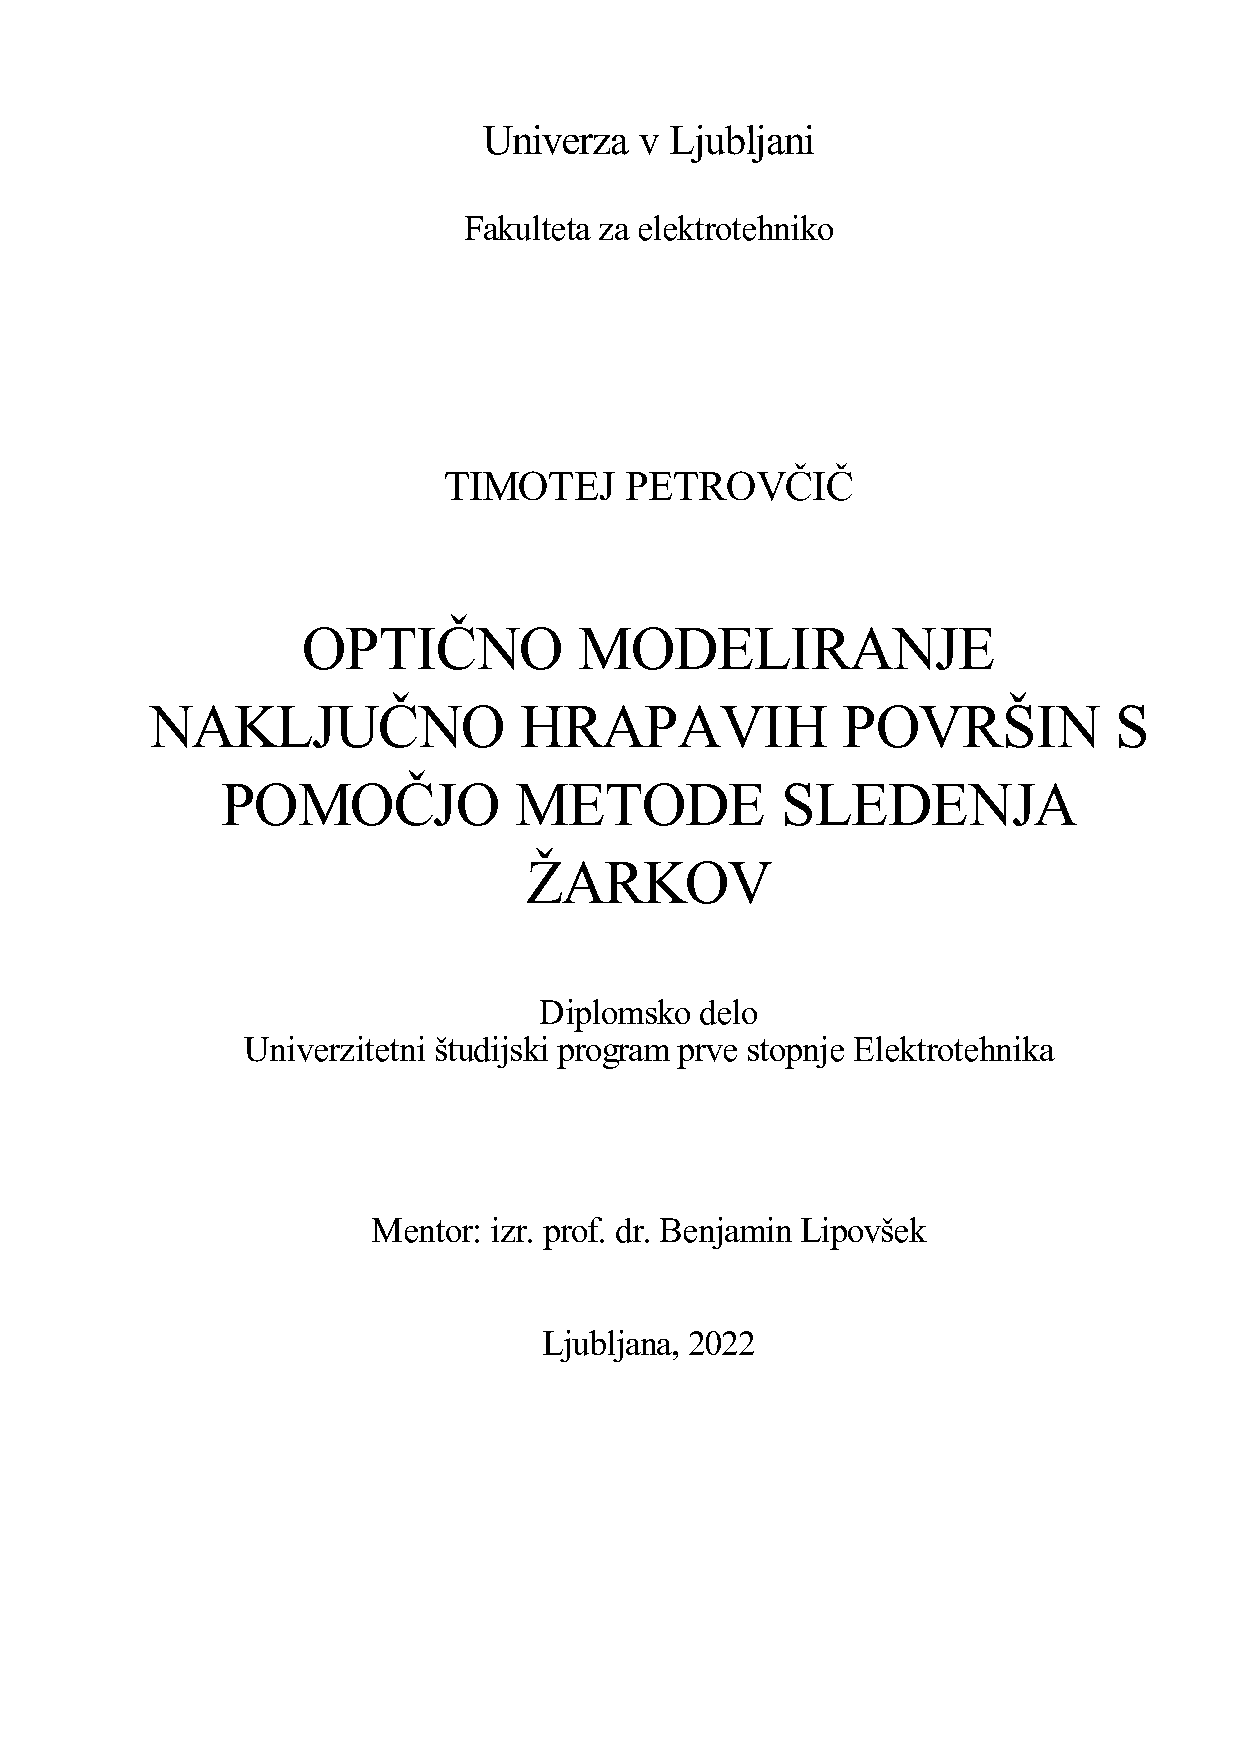
\includepdf[pages={1},fitpaper]{NaslovnaStranDiplome.pdf}
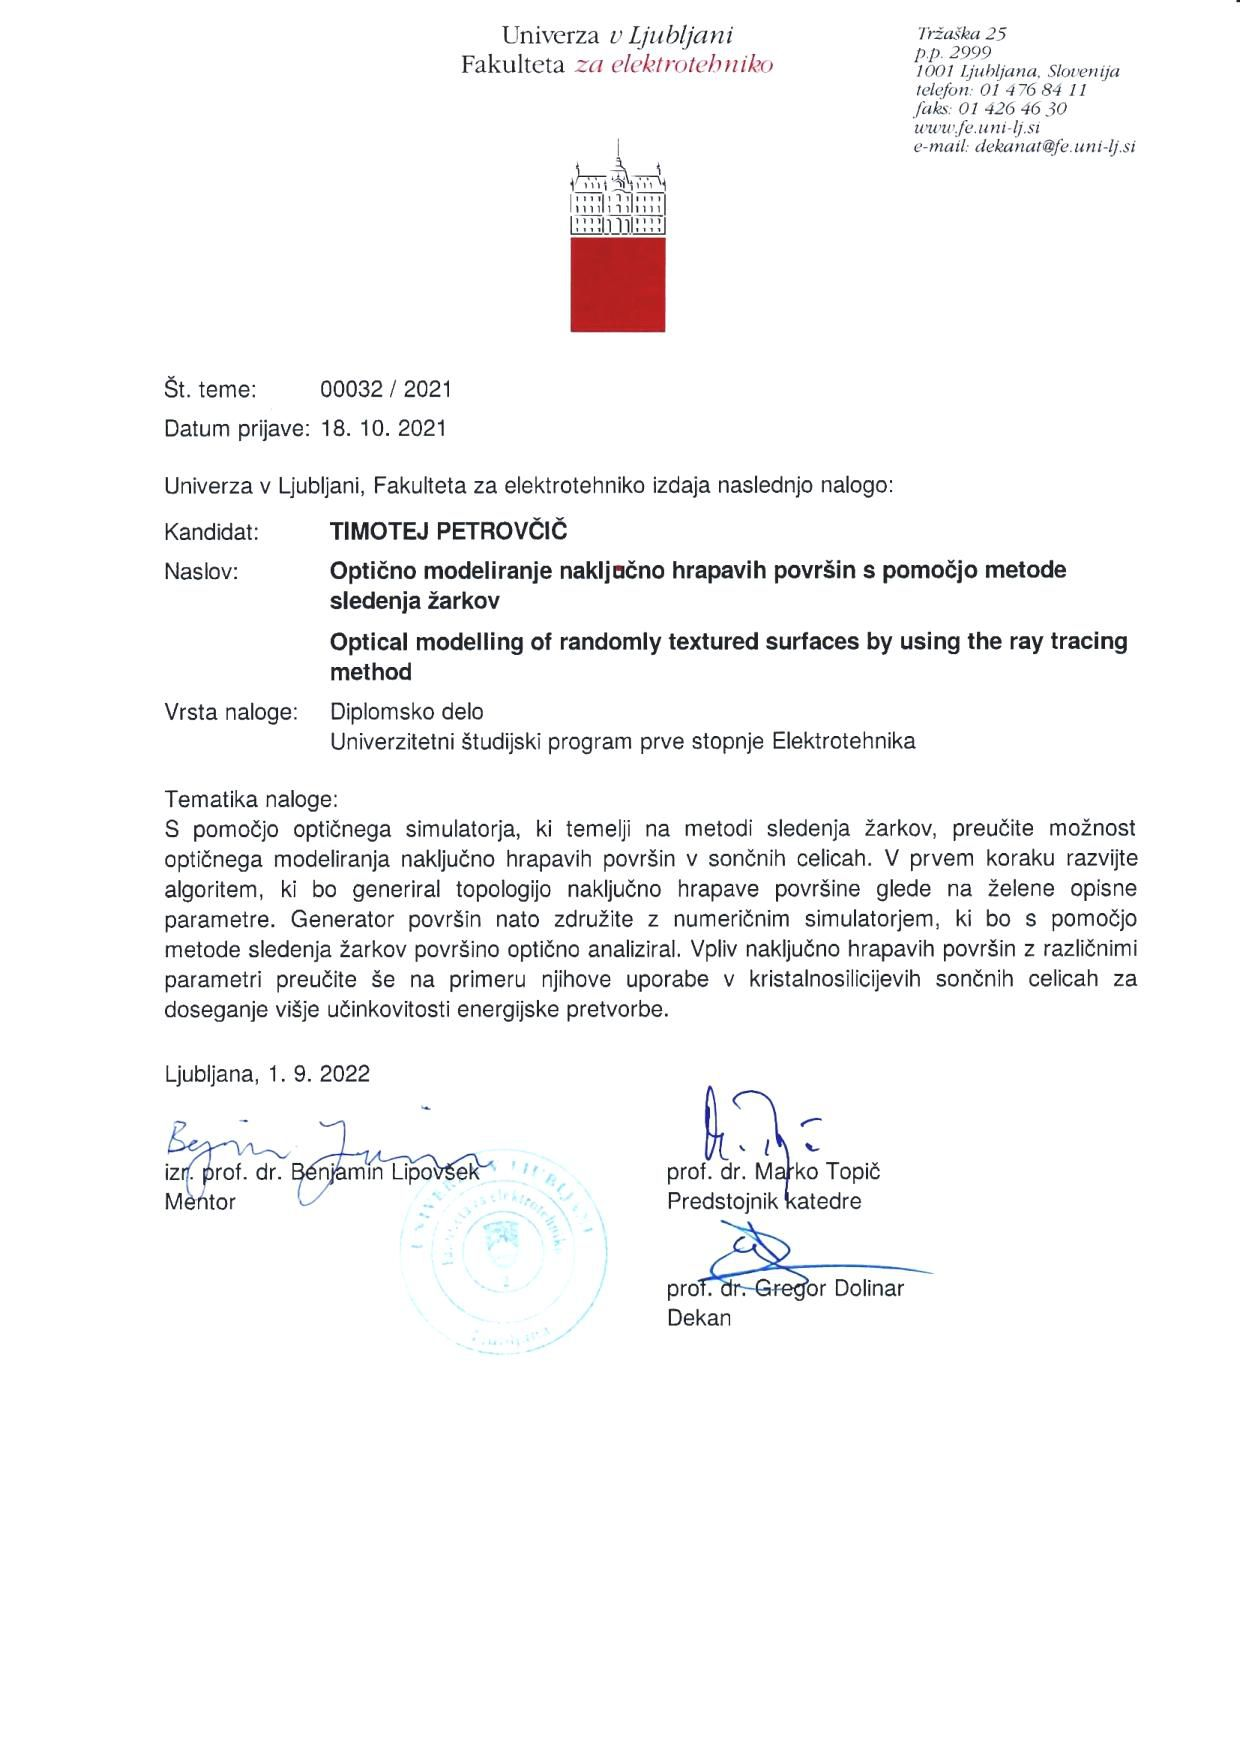
\includepdf[pages={1},fitpaper]{potrdiloKatedre.pdf}
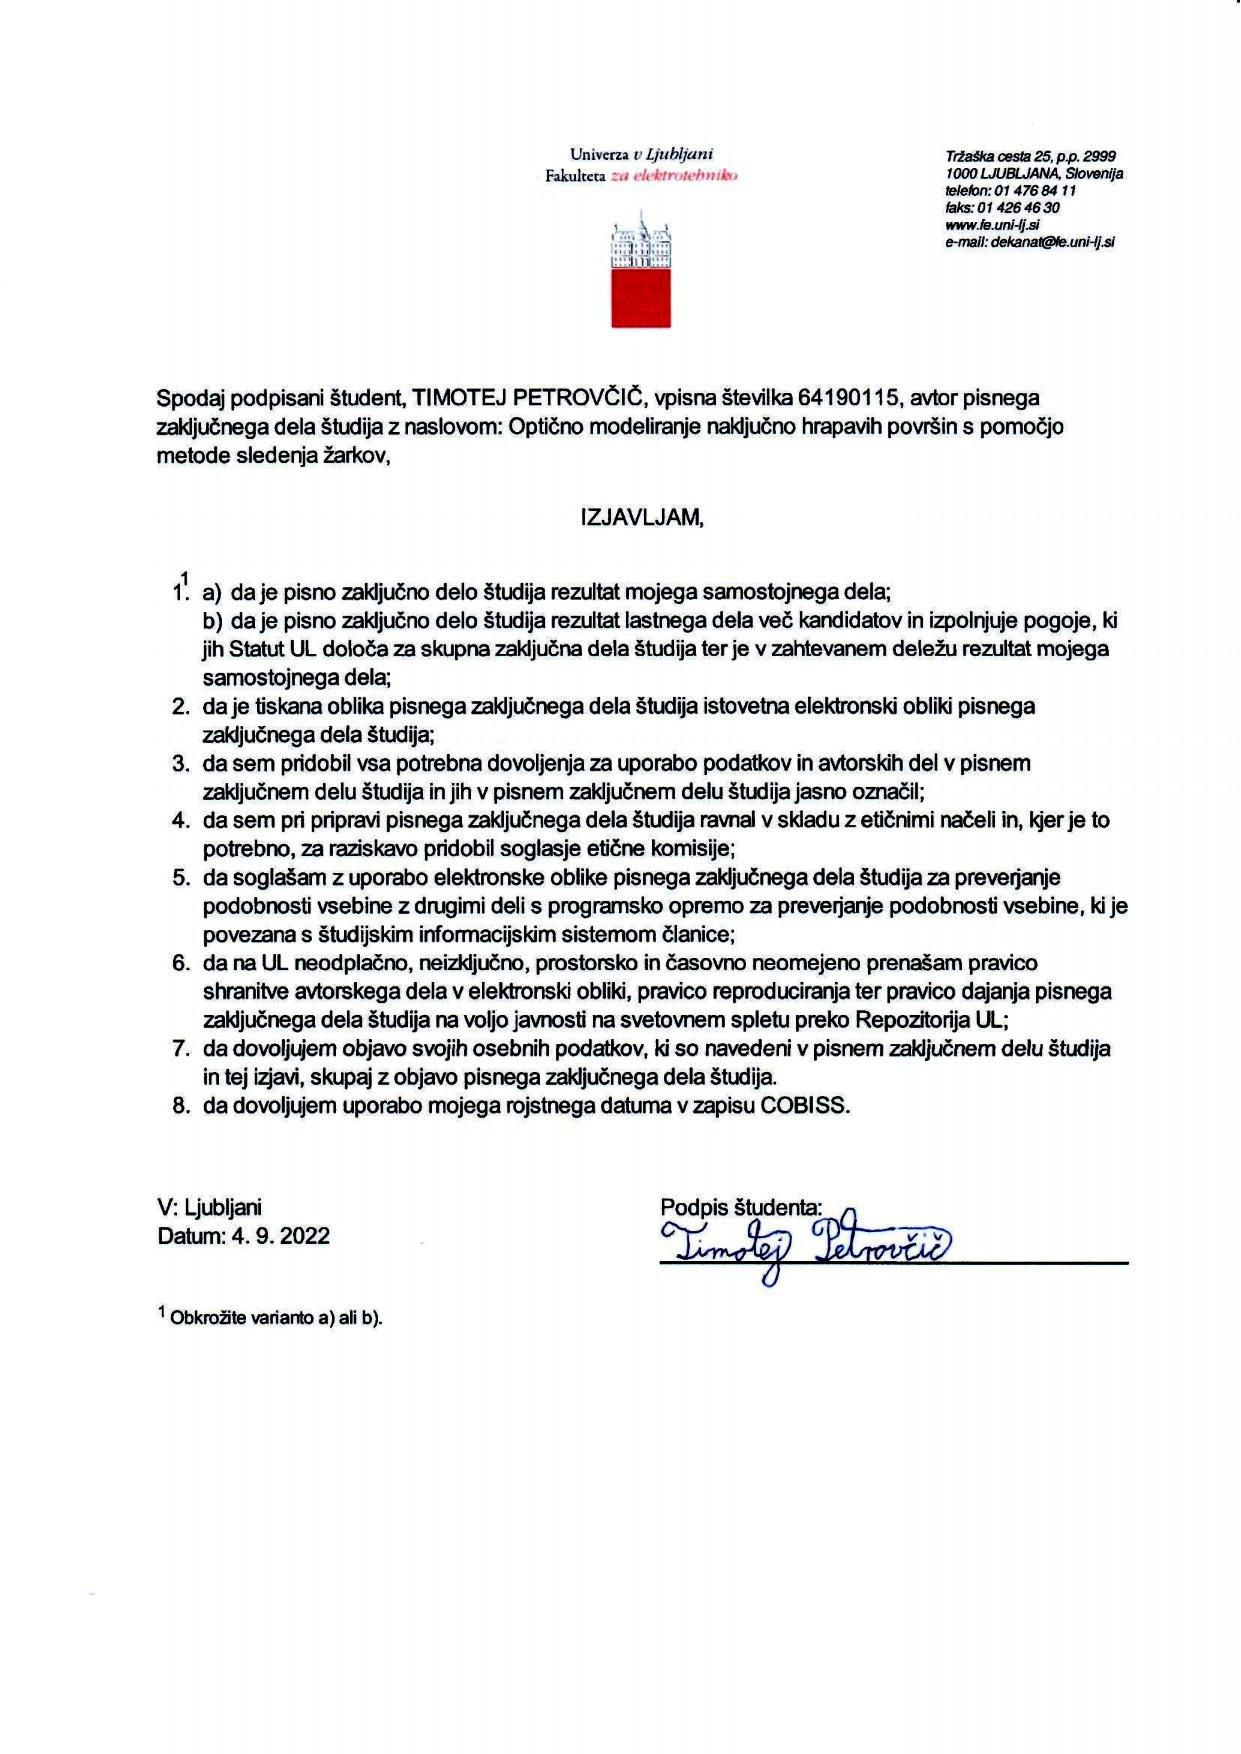
\includepdf[pages={1},fitpaper]{izjavaOAvtorstvu.pdf}

%******************************* NASLOVNICA ************************************
\maketitle

%******************************* ZAHVALA ***************************************
\zahvala
Zahvaljujem se mentorju izr. prof. dr. Benjaminu Lipovšku za pomoč, predloge ter vodenje skozi proces pisanja diplomskega dela. Prav tako bi se rad zahvalil Laboratoriju za fotovoltaiko in optoelektroniko, ki mi je omogočil izposojo programske opreme. Na koncu gre zahvala še staršem, ki so mi omogočili študij ter me pri njem spodbujajo. 


%******************************* POVZETEK IN KLJUČNE BESEDE ********************
\povzetek

Diplomsko delo zajema področje modeliranja in razvoja sončnih celic. S pomočjo simulatorja CROWM (Combined Ray Optics/Wave Optics Model), ki deluje na osnovi kombinacije geometrijske in valovne optike, bomo modelirali sončne celice z različnimi naključno hrapavimi površinami med sloji materialov.

Prvotno je bil izdelan generator naključno hrapavih površin z izračunavanjem efektivne hrapavosti ter korelacijske dolžine. Omenjena parametra uporabljamo za ločevanje naključno hrapavih površin. Sledil je razvoj avtomatizacijskega programa, ki nam zaporedno generira površino ter izvede simulacijo.
Na koncu smo ovrednotili vpliv različnih naključno hrapavih površin na izkoristek simuliranih sončnih celic.


\kljucnebesede
sončna celica, CROWM (Combined Ray Optics/Wave Optics Model), naključno hrapava površina, efektivna hrapavost, korelacijska dolžina.

\selectlanguage{english}

%******************************* ABSTRACT AND KEYWORDS *************************

\abstract
The thesis covers the field of modeling and development of solar cells. With the help of the CROWM (Combined Ray Optics/Wave Optics Model) simulator, which works on the basis of geometrical and wave optics, we will model solar cells with different randomly textured surfaces between layers of materials.

Originally, a generator of randomly textured surfaces was created with calculations of the effective roughness and the correlation length. We use the mentioned parameters to separate and classify randomly textured surfaces. This was followed by the development of an automation program that sequentially generates the surface for us and performs the simulation.
Finally, we evaluated the influence of different randomly textured surfaces on the efficiency of the simulated solar cells.

\keywords
solar cell, CROWM (Combined Ray Optics/Wave Optics Model), randomly textured surface, RMS roughness, corelation length.

\selectlanguage{slovene}

%******************************* KAZALO ****************************************
\tableofcontents

%******************************* SEZNAM SLIK, SEZNAM TABEL *********************
\seznamslik
\seznamtabel

%******************************* SEZNAM SIMBOLOV *******************************
\seznamsimbolov
V pričujočem zaključnem delu so uporabljene naslednje veličine in simboli:

\begin{center}
    \begin{tabular}{*{4}{l}} \hline
        \multicolumn{2}{c}{\bf{Veličina / oznaka}}           & \multicolumn{2}{c}{\bf{Enota}} \\ \hline
        Ime                & Simbol                          & Ime      & Simbol              \\ \hline
        število žarkov                 & $N_{rays}$        & /    & /     \\
        natančnost sledenja žarkov     & $RT_{precision}$   & /    & /     \\
        hrapavost            & $R_x$             & mikrometer    & \micro m        \\
        korelacijska dolžina           & $\xi$             & mikrometer    & \micro m        \\
        kratkostični tok       & $J_{sc}$   & \parbox{5cm}{miliamper na\\kvadratni centimeter}    & $mA/cm^{2}$ \\ [10pt] \hline      
    \end{tabular}
\end{center}

\mainmatter

%******************************* UVOD ******************************************
\chapter{Uvod} \label{uvod}

Brezogljično pridobivanje električne energije je verjetno eden izmed največjih izzivov trenutne naravoslovne stroke, saj izpodbija določene že uveljavljene vire energije ter jih poskuša nadomestiti z novejšimi. Zahteve dinamične proizvodnje in odjema električne energije poleg različnih odzivnih časov zagonov in izklopitev elektrarn kompleksnost problema kvečjemu otežijo. Potreben je razvoj zelenih virov, ki rešijo dinamičnost razmer ter imajo dovolj visoke izkoristke. Eden izmed zelenih virov, ki ima glede na njegovo izkoriščenost še velik potencial, je sončna energija. \cite{Nas_stik_SAZU}

Izkoristki komercialnih sončnih celic, osnovanih na rezinah kristalnega silicija, ki predstavljajo poglavitni vir pretvorbe sončne energije v električno, se gibljejo med 15 in 25 procentov. Kljub temu, da izkoristki razvojnih večspojnih sončnih celic v določenem primeru lahko presegajo 45 procentov, se le-te za komercialne namene ne uporabljajo. Glavni razlog za neuporabo omenjenih sončnih celic je cena izdelave, ki je primarno povezana z uporabljenimi materiali in samo izdelavo. Izdelava več-plastnih strukturno razgibanih sončnih celic je zahtevna, potrebuje kompleksnejše produkcijske linije in dražjo opremo ter jo je težko uporabiti za večje površine, hkrati pa mora zadostiti cenovni konkurenčnosti trga. 

V splošnem sončne celice delimo na več kategorij in podkategorij:
\begin{itemize}
    \item glede na strukturno zgradbo silicija:
    \begin{itemize}
        \item monokristalni silicij (urejena mrežna struktura atomov)
        \item polikristalni silicij (naključna razporeditev kristalnih zrn - večji skupki monokristalnih atomov, ki so na spojih naključno usmerjeni)
    \end{itemize}
    
    \item glede na število spojev:
    \begin{itemize}
        \item enospojne celice (najvišja izkoristka 26.1\% za silicij, 27,6\% za $GaAs$)
        \begin{itemize}
            \item Uporabljeni polprevodniki: \textit{Si}, $GaAs$ 
        \end{itemize}
        \item večspojne celice (najvišji izkoristek 47,1\%)
        \begin{itemize}
            \item Uporabljeni polprevodniki: $GaInP/GaInAs/Ge$
        \end{itemize}
    \end{itemize}
    
    \item glede na debelino plasti:
    \begin{itemize}
        \item tankoplastne celice (najvišji izkoristek 23,4\%)
        \begin{itemize}
            \item Uporabljeni polprevodniki: $Cu(In, Ga)Se_2$, $CdTe$, \textit{perovskit}, \textit{amorfni Si}
        \end{itemize}
        \item debeloplastne celice (najvišji izkoristek 27,6\%)
        \begin{itemize}
            \item Uporabljeni polprevodniki: \textit{Si}, \textit{GaAs}, \textit{CdTe} 
        \end{itemize}
        \item heterospojne celice (kombinacija zgornjih dveh pristopov) (najvišji izkoristek 26,7\%)
    \end{itemize}
\end{itemize}

Zaradi prepletanja različnih tehnologij in razvoja sončnih celic se določeni materiali uporabljeni v različnih izvedbah (Glej sliko \ref{fig:izkoristki}).

Za razvoj komercialnih sončnih celic je torej potreben kompromis med dostopnostjo surovin, kompleksnostjo izdelave ter učinkovitostjo pretvorbe sončne energije v električno. Delež učinkovitost lahko pridobimo nazaj s pomočjo optimalnega oblikovanja hrapavih površin ter izbiro primernega materiala in njegove debeline.

\clearpage

\begin{figure}[H]
    \vspace{-4em}
    \centering
    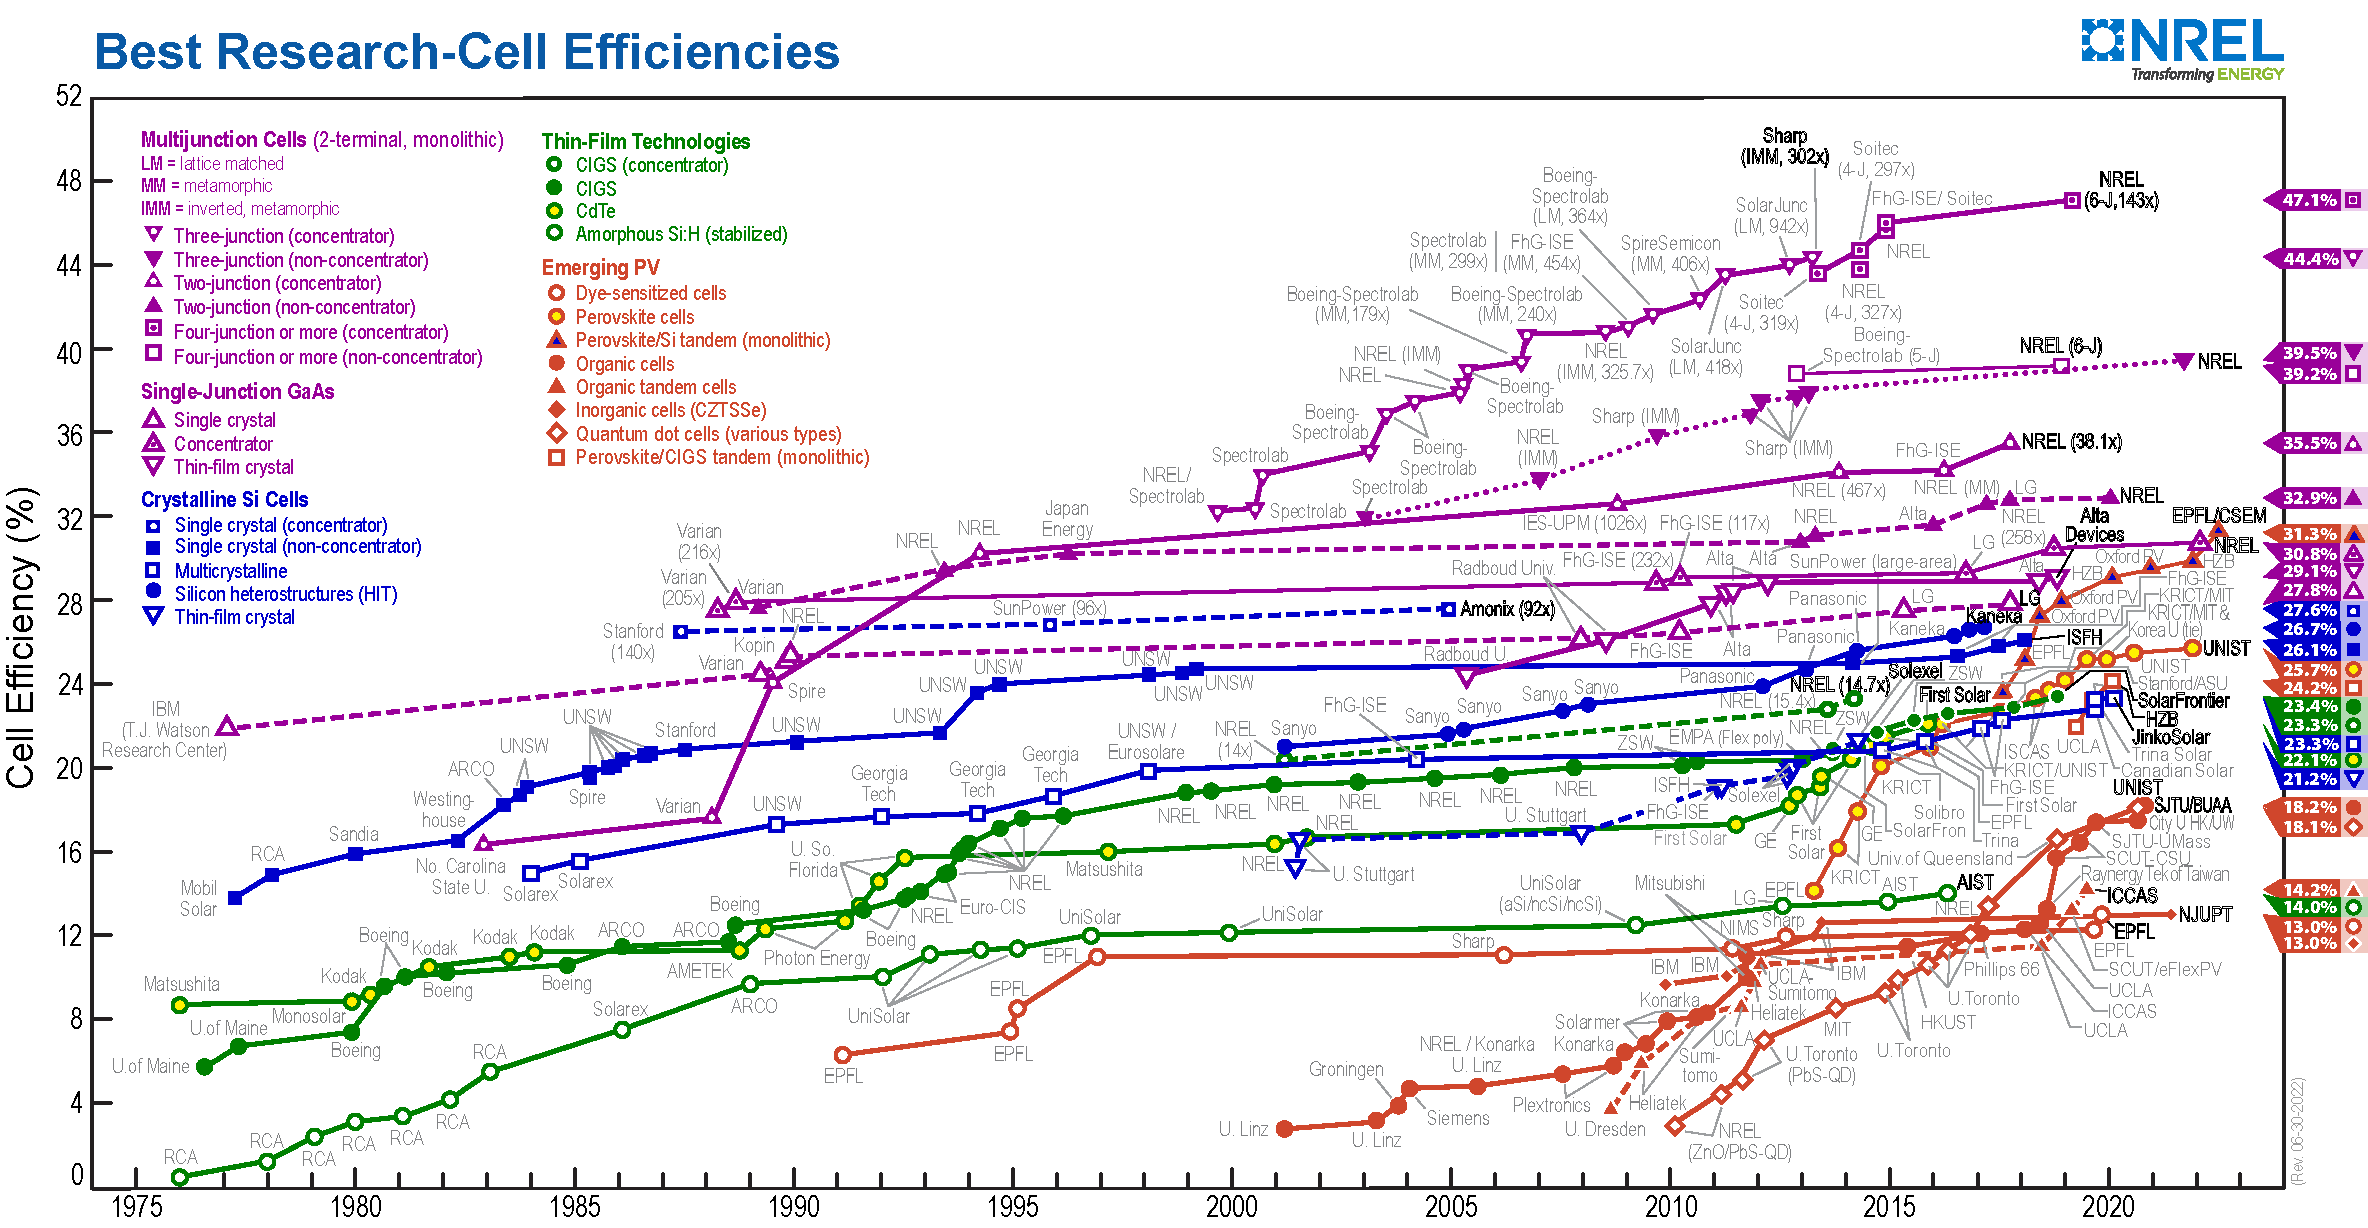
\includegraphics[width=210mm, height=140mm, angle=90]{Slike/solar-cell-graph.pdf}
    \caption[Izkoristki razvoja sončnih celic skozi zgodovino]{Izkoristki razvoja sončnih celic skozi zgodovino \footnotemark} 
    \label{fig:izkoristki}
    \vspace{-1em}
\end{figure}

\footnotetext{Slika v višji ločljivosti je dostopna: \url{https://www.nrel.gov/pv/cell-efficiency.html}}

\chapter{Predstavitev problema}

Osrednja tematika diplomskega dela je povečanje izkoristka sončnih celic na podlagi izboljšane absorpcije v optično aktivnih plasteh. Problem je obsežen in zahteva znanje večih področij. V našem primeru se bomo omejili na optimizacijo izkoristka s pomočjo naključno hrapavih površin. Omenjeno bomo izvedli z izdelavo generatorja naključno hrapavih površin v nano- in mikrometerskem območju, katerega generirane površine bomo nato s pomočjo računalniškega modeliranja na različnih optičnih strukturah analizirali.

Hrapave površine na mikro oziroma nano skali spreminjajo odbojnost površine. Ta lastnost je za nas pomembna iz vidika, da ob njeni pravilni uporabi lahko dosežemo različno odbojnost izbranih plasti v sončnih celicah. Trdimo lahko, da z uporabo hrapavih materialov odbojnost sončnih celic spremenimo za eden do dva reda velikosti.

Sedaj ko razumemo učinek hrapavosti na površino nas zanima še kako površino kvantitativno ovrednotiti. V tej točki omenimo ključne parametre, s katerimi opisujemo različne hrapavosti, oziroma bolj natančno efektivno hrapavost ter korelacijsko dolžino, ki so opisane v poglavju \ref{nanoPov}, a jih sedaj samo omenimo za lažje razumevanje. Efektivna hrapavost je vezana na višinsko razliko med vrhovi in dolinami na površini, korelacijska dolžina pa na razdaljo med ponavljajočimi podobnimi višinami. Razmerje omenjenih parametrov je torej krivec za določanje hrapavosti površine. \cite{117339} \cite{10.1002/pip.1050}

\begin{figure}[H]
    \centering
    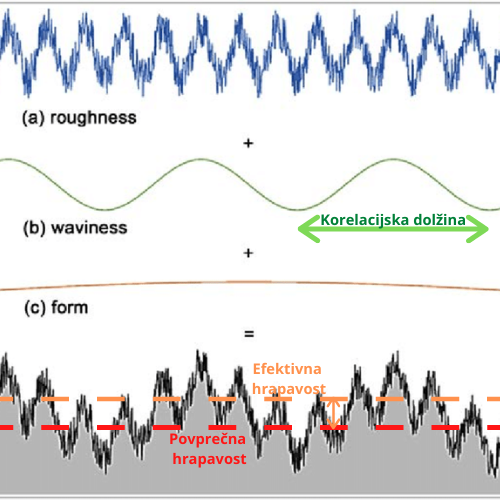
\includegraphics[scale=0.75]{Slike/rough.png}
    \caption{Grafični prikaz nastanka hrapavosti, povprečne in efektivne hrapavosti ter korelacijske dolžine \cite{roughness}}
    \label{fig:rough}
\end{figure}

Po osnovni razlagi pojava hrapavosti lahko preidemo na praktično uporabo le-te na sončnih celicah. Poglejmo zgradbo tipične kristalnosilicijeve celice strukture PERC, ki jo kasneje tudi simuliramo, ter na njej predstavimo vpliv hrapavosti površin. 


\section{Kristalnosilicijeve PERC sončne celice}
\label{percCelice}
Kristalnosilicijeve sončne celice (od sedaj naprej sončne celice) delujejo na principu elektronske asimetrije v polprevodniku, ki omogoča pretvorbo svetlobne v sončno energijo. Omenjena asimetrija je prisotna v vsakem pn-spoju, kateremu prilagodimo geometrijo ter uporabljene materiale glede na izbrano področje uporabe. Zaradi različne dopiranosti materialov se poruši električna nevtralnost ter povzroči nastanek vgrajenega električnega polja v ozkem področju okolice pn-spoja. Ohranitev nevtralnosti strukture omogoči termično ravnovesje kontaktne in difuzijske napetosti.

Osvetlitev spoja povzroči generacijo presežnih parov elektronov in vrzeli. Zaradi nesimetrije mobilnosti nosilcev naboja zaradi vgrajenega električnega polja so generirani elektroni pospešeni iz področja tipa p v področje tipa n ter vrzeli iz področja tipa n v področje tipa p. Ob kratkostični sklenitvi ozimroma sklenitvi zunanjih priključkov spoja preko bremena nastane zaradi usmerjenega gibanja nosilcev električni tok skozi zunanje sponke (slika \ref{fig:delovanje}). Generirani tok se prišteva temni diodni karakteristiki in povzroči premik diodne karakteristike v negativne vrednosti po tokovni osi ter nam potrdi, da električno energijo sončna celica oddaja (slika \ref{fig:karakteristika}). Tokovno napetostno karakteristiko opiše enačba:

\[I = I_{S}(e^{ \tfrac{U}{U_{T}} } - 1) - I_{L} \]

\noindent kjer je $I_{S}$ tok nasičenja idealnega stopničastega pn-spoja in $I_{L}$ svetlobno generiran tok. V kontekstu sončnih celic so podatki o toku navadno normirani s površino celice, govorimo torej o tokovnih gostotah $J_S$ ter $J_L$.

\begin{figure}[H]
    \centering
    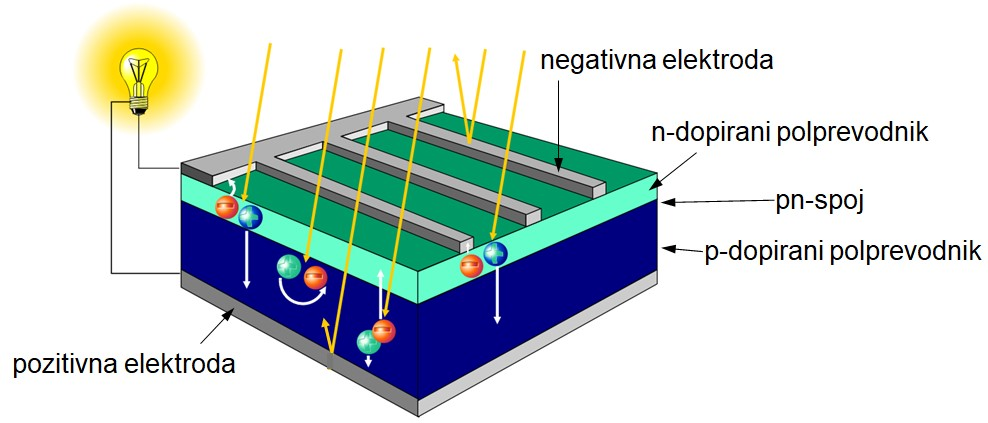
\includegraphics[width=120mm, height=36mm]{Slike/solar_cell.jpg}
    \caption{Delovanje sončne celice \cite{predavanjaopto}}
    \label{fig:delovanje}
\end{figure}

\begin{figure}[H]
    \centering
    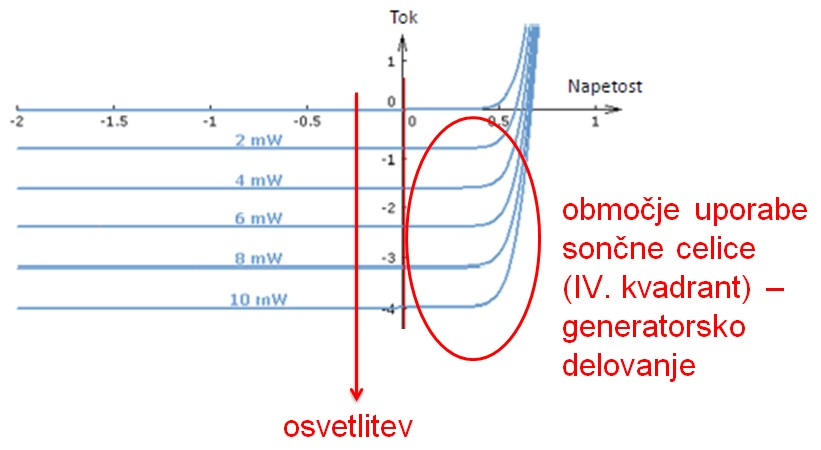
\includegraphics[width=100mm, height=36mm]{Slike/characteristic.jpg}
    \caption{Tokovno napetostna karakteristika diode in sončnih celic \cite{predavanjaopto}}
    \label{fig:karakteristika}
\end{figure}

Običajni izhodni parametri sončnih celic so:
\begin{itemize}
    \item gostota kratkostičnega toka ($\bf J_{sc}$)
    \item napetost odprtih sponk ($\bf U_{OC}$)
    \item polnilni faktor ($\bf FF$)
\end{itemize}

Izmed omenjenih parametrov nas v primeru simulacij zanima kratkostični tok, saj na tega vplivajo optične razmere v sončni celici. \cite{polprevodniskaelektronika}

Kratkostični tok v idealnih pogojih določa vsak foton, katerega energija je večja od širine energijske reže polprevodnika. Torej je kratkostični tok pogojen s fluksom oziroma pretokom fotonov. Pretok fotonov lahko izračunamo iz energijske porazdelitve sončne svetlobe z deljenjem energijske vsebine pri dani valovni dolžini z energijo fotonov pri enaki valovni dolžini. Največji kratkostični tok dobimo z integracijo omenjene porazdelitve po vseh valovnih dolžinah, pri katerih se pri dani energijski reži še vedno lahko generira par elektron-vrzel. V primeru silicija je energijska reža široka $1,1\ eV$ ter je največja valovna dolžina, ki se še lahko absorbira, $1,13\ \mu m$. Z ožanjem širine energijske reže kratkostična tokovna gostota narašča, saj število fotonov z zadostno energijo za kreiranje parov elektron-vrzel narašča. 

V simulacijah tega diplomskega dela smo uporabili PERC (Pasivated emitter rear cell) strukturo sončnih celic, katere osnova je pn spoj. Vpadna površina celice je običajno strukturirana z naključnimi piramidami (struktura hrapavosti v našem primeru ni piramidna), ki so izdelane z anizotropnim jedkanjem silicijeve rezine. Piramidna površina povzroči zmanjšanje odbojnosti ter spremeni vpadni kot svetlobe v polprevodniku. Poševen kot omogoči absorpcijo svelobe bližje pn-spoju. Podobno je strukturirana tudi zadnja površina celice, ki dolgovalovno neabsorbirano svetlobo odbija nazaj v optično aktivno plast celice. Odbojnost zadnje strani celice izboljša tudi plast kovine, ki deluje kot zrcalo ter povzroča nastanek termičnega oksida, ki zmanjša gostoto površinskih stanj in s tem poveča hitrost površinskih rekombinacij. \cite{fotonskielementi}

\clearpage

Končna struktura PERC, ki smo jo obravnavali v simulacijah je sledeča: (od zgoraj navzdol):

\begin{minipage}{.5\linewidth}
\vspace{-30pt}
\begin{itemize}
    \item steklo 
    \begin{itemize}
        \item debelina plasti: $\bf 3,2\ mm$
    \end{itemize}
    \item EVA folija (etilen-vinil acetat)
    \begin{itemize}
        \item debelina plasti: $\bf 0,5\ mm$
    \end{itemize}
    \item silicijev nitid ($SiN_x$) 
    \begin{itemize}
        \item debelina plasti: $\bf 70\ nm$
    \end{itemize}
    \item kristalni silicij (optično aktivna plast, hrapava površina na obeh straneh)
    \begin{itemize}
        \item debelina plasti: $\bf 0,18\ mm$
    \end{itemize}
    \item aluminijev oksid ($Al_2O_3$)
    \begin{itemize}
        \item debelina plasti: $\bf 10\ nm$
    \end{itemize}
    \item silicijev nitrid ($Si_3N_4$)
    \begin{itemize}
        \item debelina plasti: $\bf 100\ nm$
    \end{itemize}
    \item aluminij ($Al$)
    \begin{itemize}
        \item debelina plasti: $\bf 1000\ nm$
    \end{itemize}
\end{itemize}
\end{minipage}
\hfill
\begin{minipage}{.5\linewidth}
\vspace{-20pt}
\begin{figure}[H]
    \centering
    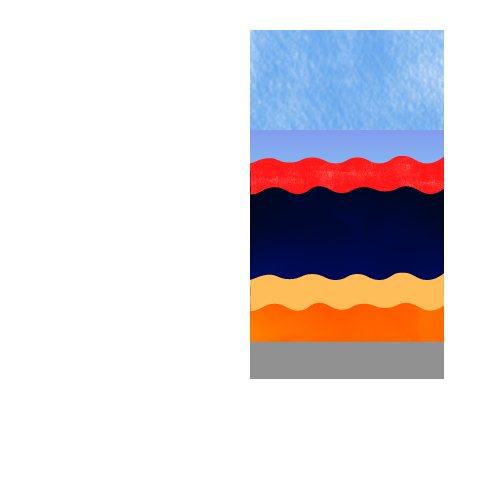
\includegraphics[trim={170 90 40 20}, clip, height=2.2\linewidth,  width=.6\linewidth]{Slike/PERC_struktura.png}
    \caption{Plasti PERC celice}
    \label{fig:my_label}
\end{figure}
\end{minipage}
\vspace{5pt}


\section{Modeliranje sončnih celic}

Modeliranje sončnih celic nam omogoča lažje in cenejše računalniško podprto načrtovanje kompleksnih struktur. Poznamo več principov modeliranja sončnih celic. Glede na uporabljen fizikalni model generalno ločimo več pristopov:

\begin{itemize}
    \item pristop z nadomestnim modelom
    \item pristop z modelom geometrijske optike (lažji izračuni, večje število izračunov)
    \item pristop z modelom valovne optike (težji izračuni, manjše število izračunov)
    \item mešani pristop (kombinacija zgoraj omenjenih)
\end{itemize}

Omenjene fizikalne modele se lahko rešuje na več načinov. V spolšnem zahtevajo različne numerične metode ter jih je mogoče izvajati v eni, dveh ali treh dimenzijah. Izbranemu modelu in geometriji se zahtevnost izvedbe sorazmerno spreminja.\cite{10.1016/J.SOLMAT.2014.09.026} Pogosto uporabljene numerične metode za modeliranje optičnih pojavov so:
\begin{itemize}
    \item metode sledenja žarkov
    \item metode matričnih opreacij (npr. metoda prenosnih matrik)
    \item metode rigoroznega reševanja diferencialnih enačb (npr. metoda končnih elementov)
    \item ostale
\end{itemize}



\subsection{Simulator CROWM}

\begin{quote}
„Optični simulator CROWM, kombinirani žarčno optični/valovno optični model, je bil razvit v Laboratoriju za fotovoltaiko in optiko, Fakultete za elektrotehniko. Omogoča optične simulacije več-plastnih optoelektronskih struktur sestavljenih iz debele (nekoherentne) plasti in poljubnega števila tankih (koherentnih) plasti. Debela plast je lahko gladka ali hrapava na eni ali obeh straneh s poljubno eno-dimenzionalno ali dvo-dimenzionalno hrapavo površino, pri čemer so dimenzije hrapavosti površine reda mikrometrov ali milimetrov.

Pod glavne vhodne podatke tipične CROWM simulacije sodijo:

\begin{itemize}
    \item pogoji osvetlitve
    \item geometrija strukture
    \item optične lastnosti materialov
\end{itemize}

Izhodni podatki so totalna odbojnost in totalna prepustnost celotne strukture ter absorpcija v vsaki izmed plasti. Na podlagi absorpcije v aktivni plasti je ob upoštevanju vpadnega spektra izračunana tudi idealna gostota kratkostičnega toka ($\bf J_{sc}$), ki bi se v sončni celici generirala. V našem primeru smo za izračun upoštevali referenčni AM1.5 sončni spekter.

CROWM je zasnovan kot kombinacija dveh numeričih pristopov k optični analizi debelih in tankih plasti v simulirani strukturi: Širjenje svetlobe skozi vpadni medij, debelo teksturirano plast in izhodni medij je obravnavano s pomočjo metode sledenja žarkov v treh dimenzijah (geometrijska optika). Vpadna svetloba z določeno optično močjo in vpadnim kotom se razdeli v število diskretnih žarkov, ki se nato sledijo skozi strukturo. Moč in smer vsakega žarka je določena s profilom teksture, z absorpcijo v materialih ter z odbojnostmi na mejah med debelo plastjo in tankoplastnimi komponentami. Širjenje svetlobe skozi tanke plasti pa je analizirano s pomočjo metode prenosnih matrik (valovna optika), ki upošteva vse pojave koherentnega širjenja, kot sta destruktivna in konstruktivna interferenca.“ (Citirano po \cite{web_page}) \cite{ISSN0352-9045}   
\end{quote} 

Pri našem delu smo se osredotočili na dva parametra od katerih je rezultat simulacij pretežno odvisen. To sta število žarkov ($\bf N_{rays}$) in natančnost sledenja žarkov ($\bf RT_{precision}$).

Število žarkov simulatorju določi, koliko naključno generiranih žarkov bo poslanih skozi izbrano strukturo. Naključnost žarkov je določena z njihovim izvorom, izhodnim kotom ter močjo.

Natančnost sledenja žarkov simulatorju določi, pri kakšnem razmerju moči med trenutno močjo in vhodno močjo žarka bo žarek simulator še spremljal. Natančnost določa prag relativne moči, pri katerem žarki usahnejo. Ob dovolj majhnem razmerju med omenjenima količinama simulator prekine sledenje določenega žarka, saj ni več relevanten za izhodni kratkostični tok ter lahko njegov prispevek zanemarimo. \cite{SOM}


\section{Hrapave površine}
\label{nanoPov}
Pod pojem hrapavih površin spadajo strukturno razgibane površine v različnih velikostnih skalah, med 0,1 ter 100 nanometrov - nanohrapave površine, med 0,1 ter 100 mikrometrov - mikrohrapave površine ipd. Sestavljene so lahko iz različnih materialov, ki v kombinaciji s hrapavostjo omogočajo različne lastnosti. Podrobneje smo obravnavali različne hrapavosti in korelacijsko dolžino površine.

Hrapavost površine je definirana kot analitična mera odstopanj v smeri vektorja normale glede na idealno ravno površino. Glede na velikost parametrov hrapavosti določimo gladkost oziroma grobost površine. Hrapavost ponavadi predstavlja vnos visoko frekvenčne komponente v površino, torej lahko s pomočjo frekvence in amplitude določimo parametre za specifično površino, ki jo potrebujemo. Poznamo različne vrste hrapavosti. Splošne formule so:
\begin{itemize}
    \item Povprečna hrapavost: 
    \begin{itemize}
        \item ena dimenzija:     \[R_{a} = \frac{1}{l_{r}} \int_{0}^{l_{r}} |z(x)| dx\]
        \item \hyperref[fig:SaSq]{dve dimenziji:}     \[S_{a} = \frac{1}{A_{xy}}\ \int_{0}^{l_{x}} \int_{0}^{l_{y}} |Z(x,y)| dx dy\] 
    \end{itemize}
    
    \clearpage
    
    \item Efektivna hrapavost:
    \begin{itemize}
        \item ena dimenzija:     \[R_{q} = \sqrt{\frac{1}{l_{r}} \int_{0}^{l_{r}} z(x)^2 dx}\]
        \item \hyperref[fig:SaSq]{dve dimenziji:}     \[S_{q} = \sqrt{\frac{1}{A_{xy}}\ \int_{0}^{l_{x}} \int_{0}^{l_{y}} Z^2(x,y) dx dy}\]
    \end{itemize}
    
    
    \item Maksimalna globina dolin:
    \begin{itemize}
        \item ena dimenzija:     \[R_{v} = |min\ z(x)|\]
        \item \hyperref[fig:SvSp]{dve dimenziji:}     \[S_{v} = |min\ Z(x, y)|\]
    \end{itemize}
    
    
    \item Maksimalna višina vrhov:
    \begin{itemize}
        \item ena dimenzija:     \[R_{p} = max\ z(x)\]
        \item \hyperref[fig:SvSp]{dve dimenziji:}     \[S_{p} = max\ Z(x, y)\]
    \end{itemize}
    
    
    
    \item Maksimalna razlika med dolinami in vrhovi:
    \begin{itemize}
        \item ena dimenzija:     \[R_{z} = R_{v} + R_{p}\]
        \item \hyperref[fig:Sz]{dve dimenziji:}     \[S_{z} = S_{v} + S_{p}\]
    \end{itemize}
    
\end{itemize}

Funkcija $z(x)$ predstavlja enodimenzionalni profil oziroma $Z(x,y)$ povprečni profil v primeru dvodimenzionalne analize površine. $R_{v}$/$S_{v}$, $R_{p}$/$S_{p}$ in $R_{z}$/$S_{z}$ so definirane kot globine, višine in razlike glede na aritmetično sredino vrednosti površine. Poleg omenjenih parametrov obstaja še mnogo ostalih, ki opišejo določeno karakteristiko površine. \cite{SR} \cite{real_SR}

\begin{figure}[htp]
    \centering
    \subfigure[]{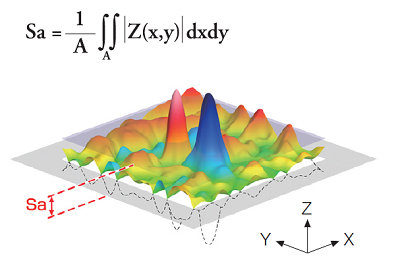
\includegraphics[width=0.49\textwidth]{Slike/S_a.png}}
    \subfigure[]{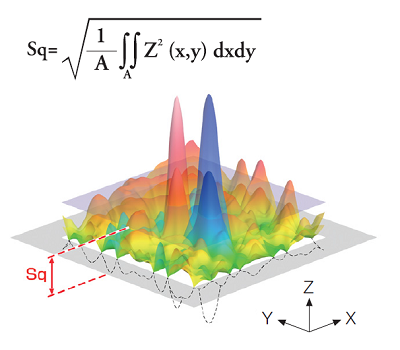
\includegraphics[width=0.49\textwidth]{Slike/S_q.png}}
    \caption{(a) Povprečna hrapavost, (b) Efektivna hrapavost \cite{real_SR}}
    \label{fig:SaSq}
\end{figure}

\begin{figure}[htp]
    \centering
    \subfigure[]{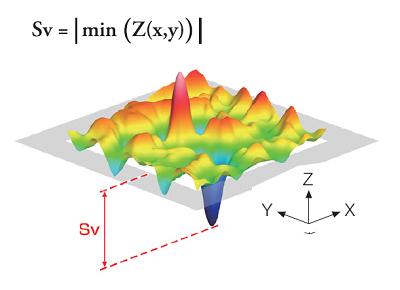
\includegraphics[width=0.49\textwidth]{Slike/S_v.png}}
    \subfigure[]{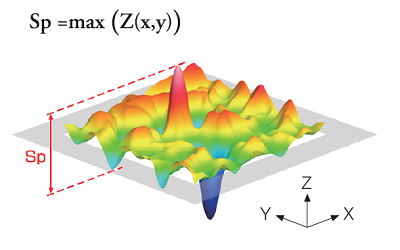
\includegraphics[width=0.49\textwidth]{Slike/S_p.png}}
    \caption{(a) Maksimalna globina dolin, (b) Maksimalna višina vrhov \cite{real_SR}}
    \label{fig:SvSp}
\end{figure}

\begin{figure}[H]
    \centering
    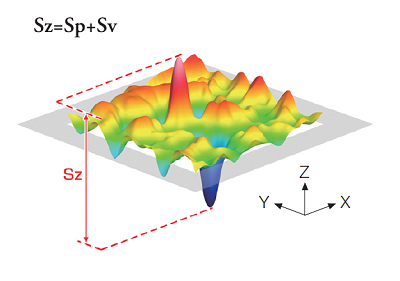
\includegraphics{Slike/S_z.png}
    \caption{Maksimalna razlika med dolinami in vrhovi \cite{real_SR}}
    \label{fig:Sz}
\end{figure}

Korelacijska dolžina predstavlja povprečno mero amplitudnih premikov med sosednjimi točkami na površini. Sam koncept korelacijske dolžine je sicer mnogo širši, saj predstavlja spremembo skalarnega polja glede na izbrani dve dolžini oziroma predstavlja korelacijo ali avtokorelacijo podanega polja. \cite{FRANCESCHETTI200721}  \cite{physicStackExchange} Definicija prihaja iz enačbe za splošno koreacijsko funkcijo:

\[ C(r, \tau) = \langle s_1(R,t) \cdot s_2(R+r,t+\tau) \rangle - \langle s_1(R,t) \rangle \langle s_2(R+r,t+\tau) \rangle \]

V zgronji funkciji je $\tau = 0$, saj se povrišna skozi čas ne spreminja, $R$ in $r$ predstavljata lokacijo na površini ter premik v sosednjo točko, $s_1$ in $s_2$ pa predstavljata funkciji amplitude. Oglati oklepaji predstavljajo termično povprečje, saj se omenjena funkcija uporablja za študije odvisnosti fizikalnih spremenljivk v termodinamiki. \cite{corelation} V realnosti se za namene izračunov omenjene količine za hrapave površine uporablja sledeča izpeljava:

\[ C(\xi) = \frac{C(0)}{e} = \frac{R_q^2}{e}\]

kjer je $C$ korelacijska funkcija, $\xi$ korelacijska dolžina in $R_q$ efektivna hrapavost. Korelacijska dolžina za hrapave površine je torej parametrizacija korelacijske funkcije in predstavlja razdaljo, pri kateri vrednost korelacije pade pod obratno vrednost Eulerjevega števila. \cite{ACL} \cite{CL}

\begin{figure}[H]
    \centering
    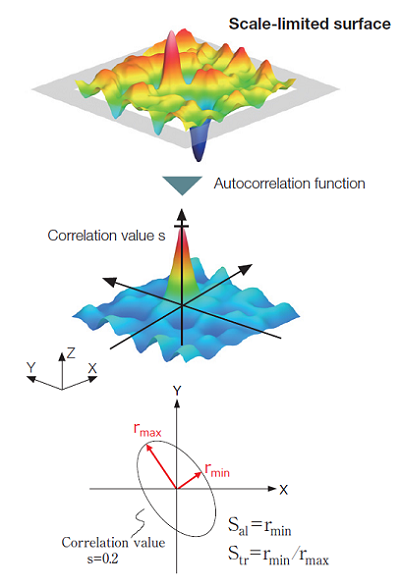
\includegraphics[scale=0.45]{Slike/CL.png}
    \caption{Avtokorelacija v dveh dimenzijah površine \cite{real_SR}}
    \label{fig:Avtokorelacija}
\end{figure}






%******************************* POGLAVJA **************************************
\chapter{Generator naključno hrapavih površin}

Generator naključno hrapavih površin (od sedaj naprej generator) je bil razvit kot pomožno orodje za modeliranje in vrednotenje. Izdelan je bil v programskem paketu MATLAB, ki nam omogoča hiter razvoj ter jasen prikaz podatkov. Prvotno je bil generator razvit kot samostojna aplikacija z grafičnim vmesnikom, a smo grafični vmesnik pri avtomatiziranem procesu izvajanja simulacij opustili.

Izhod generatorja je matrika potencialov (tabela numeričnih vrednosti višin površine v določeni točki, besedna zveza omogoča strnjen zapis), izračunane vrednosti hrapavosti naključno hrapave površine ter njena korelacijska dolžina. Vsi podatki so zapisani v formatu, ki jih lahko sprejme simulator CROWM.

\section{Sestava in delovanje programa}

Program je zgrajen modularno in omogoča hiter vklop oziroma izklop funkcij, tako v kodi kot grafičnem vmesniku. V splošnem je program razdeljen na 6 delov:

\begin{itemize}
    \setlength\itemsep{0.1em}
    \item \hyperref[gui]{Grafični vmesnik}
    \item \hyperref[osnovniGenerator]{Osnovni generator}
    \item \hyperref[predelavaPodatkov]{Predelava podatkov}
    \item \hyperref[zgoščevalnikTočk]{Zgoščevalnik točk} 
    \item \hyperref[izračunInPrikaz]{Izračun in prikaz parametrov generirane površine}
    \item \hyperref[zapisVBesedilo]{Zapis v besedilno datoteko}
\end{itemize}

\begin{figure}[H]
    \vspace{-4em}
    \centering
    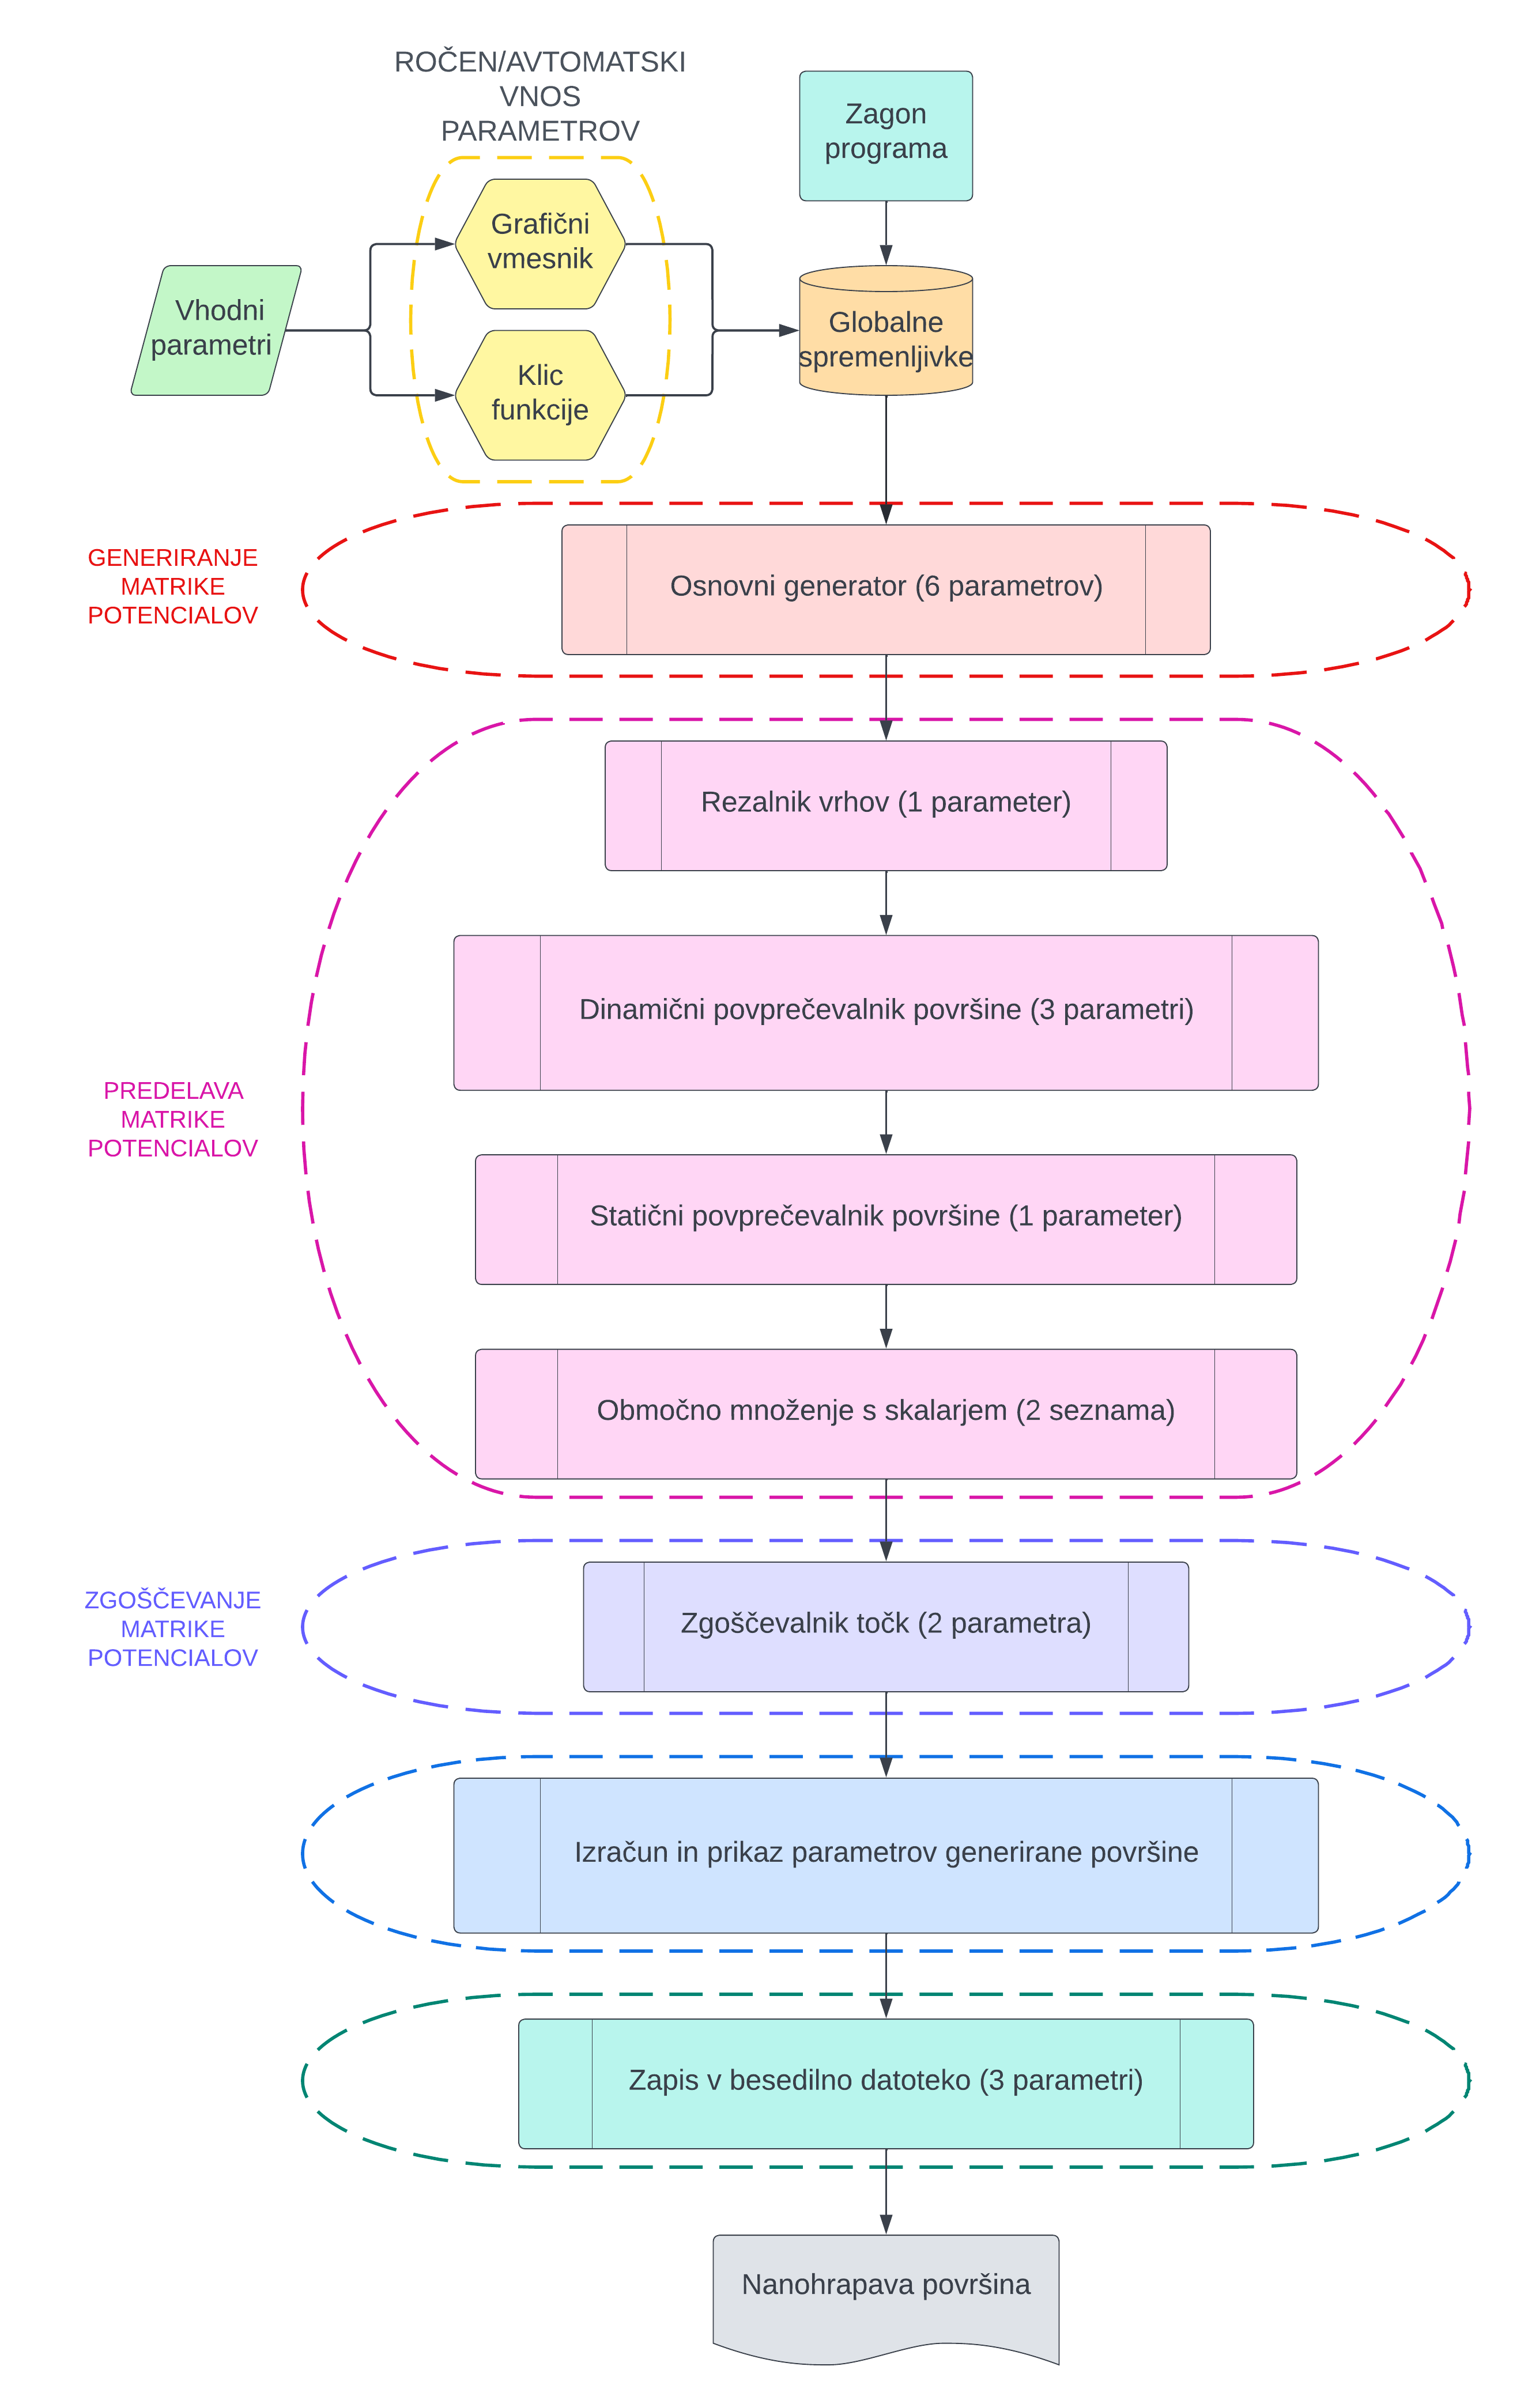
\includegraphics[width=150mm, height=220mm]{Slike/Shema programa.png}
    \caption{Shema delovanja generatorja naključno hrapavih površin}
    \label{fig:shema_delovanja_generatorja}
\end{figure}


\subsection{Vhodni parametri}

Program sprejme 18 vhodnih parametrov, s katerimi uravnavamo generacijo naključno hrapave površine. Večina jih je potrebna za predelavo podatkov, s katero lahko naključnost podatkov normaliziramo in oblikujemo. Vhodni parametri so sledeči:

\begin{itemize}
    \setlength\itemsep{0.1em}
    \item \textbf{xUm} - velikost površine v X-smeri v simulatorju CROWM
    \item \textbf{yUm} - velikost površine v Y-smeri v simulatorju CROWM 
    \item \textbf{xSize} - število elementov v X-smeri v matriki potencialov
    \item \textbf{ySize} - število elementov v Y-smeri v matriki potencialov
    \item \textbf{d\_RT} - korak premika čez površino v simulatorju CROWM
    \item \textbf{upperAmplitudeLimit} - zgornja mejna vrednost v matriki potencialov
    \item \textbf{lowerAmplitudeLimit} - spodnja mejna vrednost v matriki potencialov
    \item \textbf{deltaYLimit}  - mejna vrednost največje razlike v potencialu med sosednjima potencialoma v matriki
    \item \textbf{recursiveCumulativeSum} - število seštevka prejšnjih elementov v filtru tekočega povprečja, izvedenega na matriki potencialov 
    \item \textbf{spikeCutPercentage} - delež maksimalnih vrednosti v matriki potencialov, normiranih na dinamično izračunljivo povprečno vrednost matrike
    \item \textbf{normalSurfacePercentage} - delež velikosti pomičnega okna matrike potencialov za normalizacijo potencialov v določeno okolico vrednosti pomičnega okna
    \item \textbf{normalSurfaceFactor} - faktor za normalizacijo vrednosti znotraj pomičnega okna
    \item \textbf{normalSurfaceStepDivisor} - faktor hitrosti pomikanja vrednosti proti vrednosti pomičnega okna (možnost preskoka okolice vrednosti pomičnega okna)
    \item \textbf{fixedSurfacePercentage} - delež potencialov v matriki nastavimo na trenutno povprečno vrednost matrike potencialov
    \item \textbf{sectorCoeficientArray} - množenje matrike potencialov z matriko skalarjev, določenih z matriko deležev
    \item \textbf{sectorSizeArray} - matrika deležev, ki določajo število vrednosti matrike potencialov, množenih z določenim skalarjem iz matrike skalarjev
    \item \textbf{upscaleXSize} - število zahtevanih točk v X-smeri (poljubno nastavljanje gostote točk)
    \item \textbf{upscaleYSize} - število zahtevanih točk v Y-smeri (poljubno nastavljanje gostote točk)
\end{itemize}


\subsection{Grafični vmesnik}
\label{gui}

\hyperref[fig:gui]{Grafični vmesnik} omogoča ročni vpis vhodnih parametrov ter možnost prikaza naključno hrapave površine ter dvo-dimenzionalne Fourierove transformacije. Vmesnik ima prvotno vnešene privzete vrednosti, ki jih lahko spremenimo, pomembna je le ohranitev enakih formatov vpisa v vnosna polja programa.

\begin{figure}[H]
    \centering
    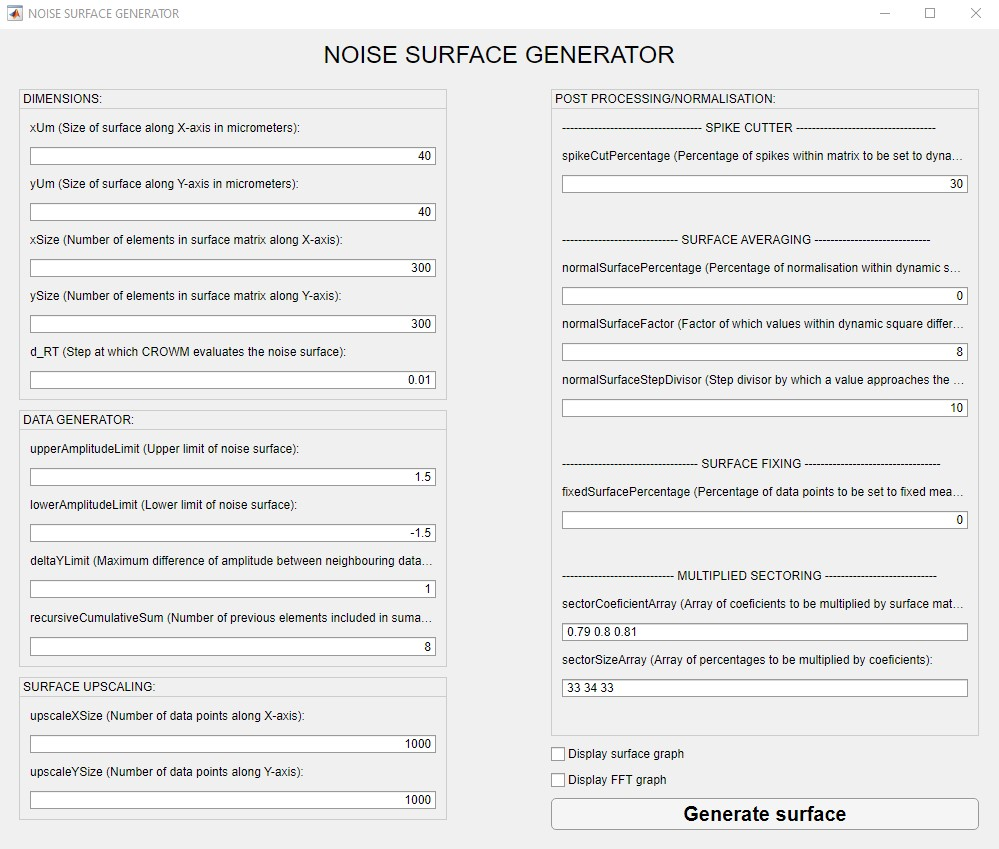
\includegraphics[width=110mm]{Slike/GUI.jpg}
    \caption{Grafični vmesnik generatorja naključno hrapave površin}
    \label{fig:gui}
\end{figure}


\subsection{Osnovni generator}
\label{osnovniGenerator}

Jedro programa je osnovni generator, ki sprejme 6 parametrov, in sicer:

\begin{itemize}
    \setlength\itemsep{0.1em}
    \item \textbf{xSize} - število elementov v X-smeri v matriki potencialov
    \item \textbf{ySize} - število elementov v Y-smeri v matriki potencialov
    \item \textbf{upperAmplitudeLimit} - zgornja mejna vrednost v matriki potencialov
    \item \textbf{lowerAmplitudeLimit} - spodnja mejna vrednost v matriki potencialov
    \item \textbf{deltaYLimit}  - mejna vrednost največje razlike v potencialu med sosednjima potencialoma v matriki
    \item \textbf{recursiveCumulativeSum} - število seštevka prejšnjih elementov v filtru tekočega povprečja, izvedenega na matriki potencialov 
\end{itemize}

\hyperref[fig:osnovniGenerator]{Osnovni generator} deluje na principu naključne generacije števil oziroma potencialov, ki jih pod določenimi pogoji vpišemo v matriko potencialov. Najprej generiramo prvi element v matriki, ki je množen s skalarjem 0,1, saj le-ta omogoči začetno vrednost potenciala v okolici števila 0. Za vsako naslednje generirano naključno število pa preverimo dva pogoja: 

\begin{itemize}
    \setlength\itemsep{0.1em}
    \item Ali je trenutno generirana vrednost v mejah med zgornjo (\textbf{upperAmplitudeLimit}) in spodnjo (\textbf{lowerAmplitudeLimit}) določeno vrednostjo glede na prvo vrednost v matriki potencialov
    \item Ali je odvod oziroma diferenca med trenutno generiranim elementom in okoliškimi elementi manjša od mejne vrednosti (\textbf{deltaYLimit})
\end{itemize}

Če sta navedena pogoja izpolnjena potem generirano število vpišemo na primerno mesto v matriki potencialov, sicer generiramo novo število in preverimo še enkrat.

\begin{figure}[H]
    \centering
    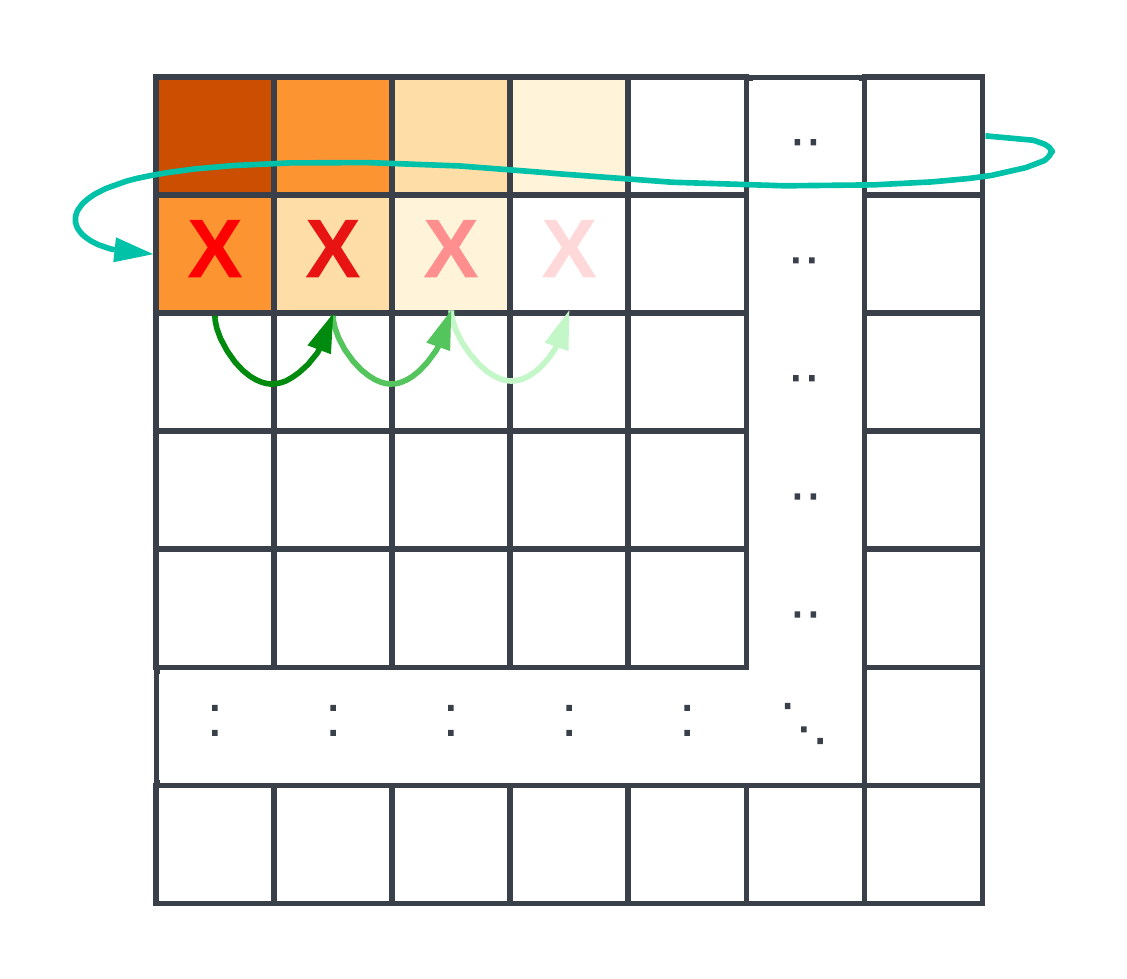
\includegraphics[width=60mm]{Slike/Osnovni generator.png}
    \caption{Delovanje naključne generacije matrike potencialov}
    \label{fig:osnovniGenerator}
\end{figure}

Na koncu izvedemo operacijo dvo-dimenzionalnega tekočega povprečja na matrki potencialov. Filter tekočega povprečja je določen z aritmetično sredino prej seštetih generiranih števil. Število prej seštetih števil je določeno s parametrom \textbf{recursiveCumulativeSum}.

Zgoraj omenjena operacija je bila dodana naknadno, saj je bilo ugotovljeno, da generirane naključno hrapave površine vsebujejo preveliko količino visoko-frekvenčnih komponent oziroma strmih vrhov, ki jih v realnosti ni mogoče izdelati.


\subsection{Predelava podatkov}
\label{predelavaPodatkov}

Predelava podatkov poteka po osnovni generaciji matrike potencialov ter na njej izvede različne globalne operacije. Globalne operacije so sledeče:

\begin{itemize}
    \setlength\itemsep{0.1em}
    \item \hyperref[rezalnikVrhov]{Rezalnik vrhov}
    \item \hyperref[dinamičniPovprečevalnik]{Dinamični povprečevalnik površine}
    \item \hyperref[statičniPovprečevalnik]{Statični povprečevalnik površine}
    \item \hyperref[območnoMnoženje]{Območno množenje s skalarjem}
\end{itemize}

Operacije se ločijo predvsem po kompleksnosti izvedbe ter časovni zahtevnosti. V določenih primerih se lahko časovna zahtevnost preveč poveča, zato je potrebno paziti pri nastavljanju vhodnih parametrov generatorja. 


\subsubsection{Rezalnik vrhov}
\label{rezalnikVrhov}

Operacija rezanja vrhov sprejme en parameter (\textbf{spikeCutPercentage}), ki določi delež rezanih vrhov, glede na število vseh elementov v matriki potencialov. Procentualna vrednost lahko preseže 100\%, saj lahko vrhove matrike porežemo večkrat. Rezalnik vrhov deluje na principu iskanja maksimalne vrednosti v matriki ter le-to nastavi na trenutno povprečno vrednost matrike.


\subsubsection{Dinamični povprečevalnik površine}
\label{dinamičniPovprečevalnik}

Operacija dinamičnega povprečevanja površine sprejme tri parametre (\textbf{normalSurfacePercentage}, \textbf{normalSurfaceFactor}, \textbf{normalSurfaceStepDivisor}). Prvi parameter predstavlja delež elementov, glede na število vseh elementov v matriki potencialov, ki določi velikost pomikajočega okna čez matriko potencialov. Znotraj pomikajočega okna primerjamo prvo vrednost v oknu z vsemi ostalimi. Če je absolutna vrednost razlike med prvo vrednostjo v oknu in vsemi ostalimi manjša od prve vrednosti, ki je množena z drugim parametrom, potem vrednost ohranimo, sicer pa glede na to ali je razlika pozitivna/negativna primerno zmanjšujemo okoliško vrednost z relativnim korakom (tretji parameter), dokler le-ta ni znotraj intervala vrednosti prvega elementa.

\begin{figure}[H]
    \centering
    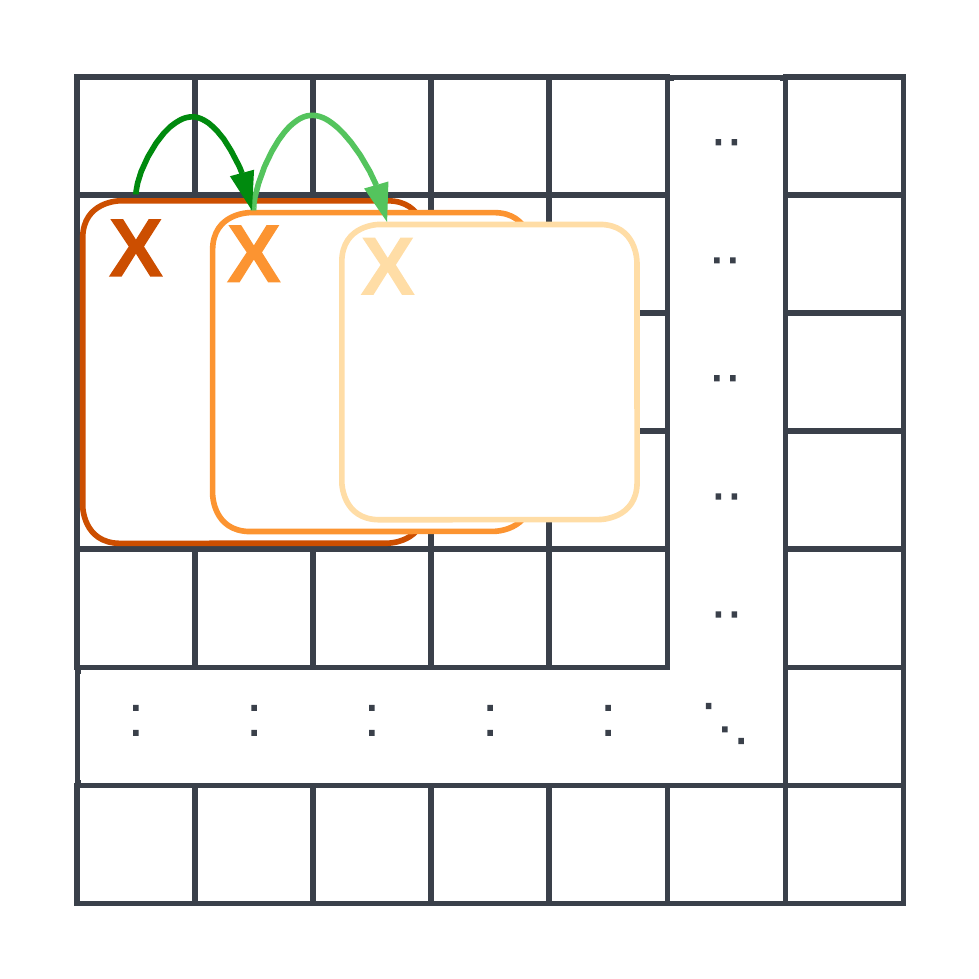
\includegraphics[width=60mm]{Slike/Dinamični povprečevalnik.png}
    \caption{Delovanje pomikajočega okna ter prikaz njegove okolice}
    \label{fig:pomikajočeOkno}
\end{figure}


\subsubsection{Statični povprečevalnik površine}
\label{statičniPovprečevalnik}

Operacija statičnega povprečevanja površine sprejme en parameter (\textbf{fixedSurfacePercentage}). Prvi parameter predstavlja delež elementov, glede na število vseh elementov v matriki potencialov, ki so nastavljeni na statično povprečno vrednost matrike potencialov, izračunano na začetku funkcije. Za preprečitev prevelikih nezveznosti v generirani matriki potencialov, algoritem poišče vrednost, ki je najbližje statični povprečni vrednosti ter eno izmed sosednjih nastavi na statično povprečno vrednost.


\subsubsection{Območno množenje s skalarjem}
\label{območnoMnoženje}

Operacija območnega množenja s skalarjem sprejme dva parametra (\textbf{sectorCoefficientArray}, \textbf{sectorSizeArray}), ki sta pravzaprav dva seznama. Prvi določi skalarje, s katerimi želimo elemente v matriki potencialov množiti, drugi pa delež elementov, glede na število vseh elementov v matriki potencialov, ki ga množimo s korespondenčnim skalarjem. Pri uporabi omenjene funkcije je potrebno paziti, da je vsota odstotkov v seznamu velikosti (\textbf{sectorSizeArray}) vedno enaka 100\%.

\begin{figure}[H]
    \centering
    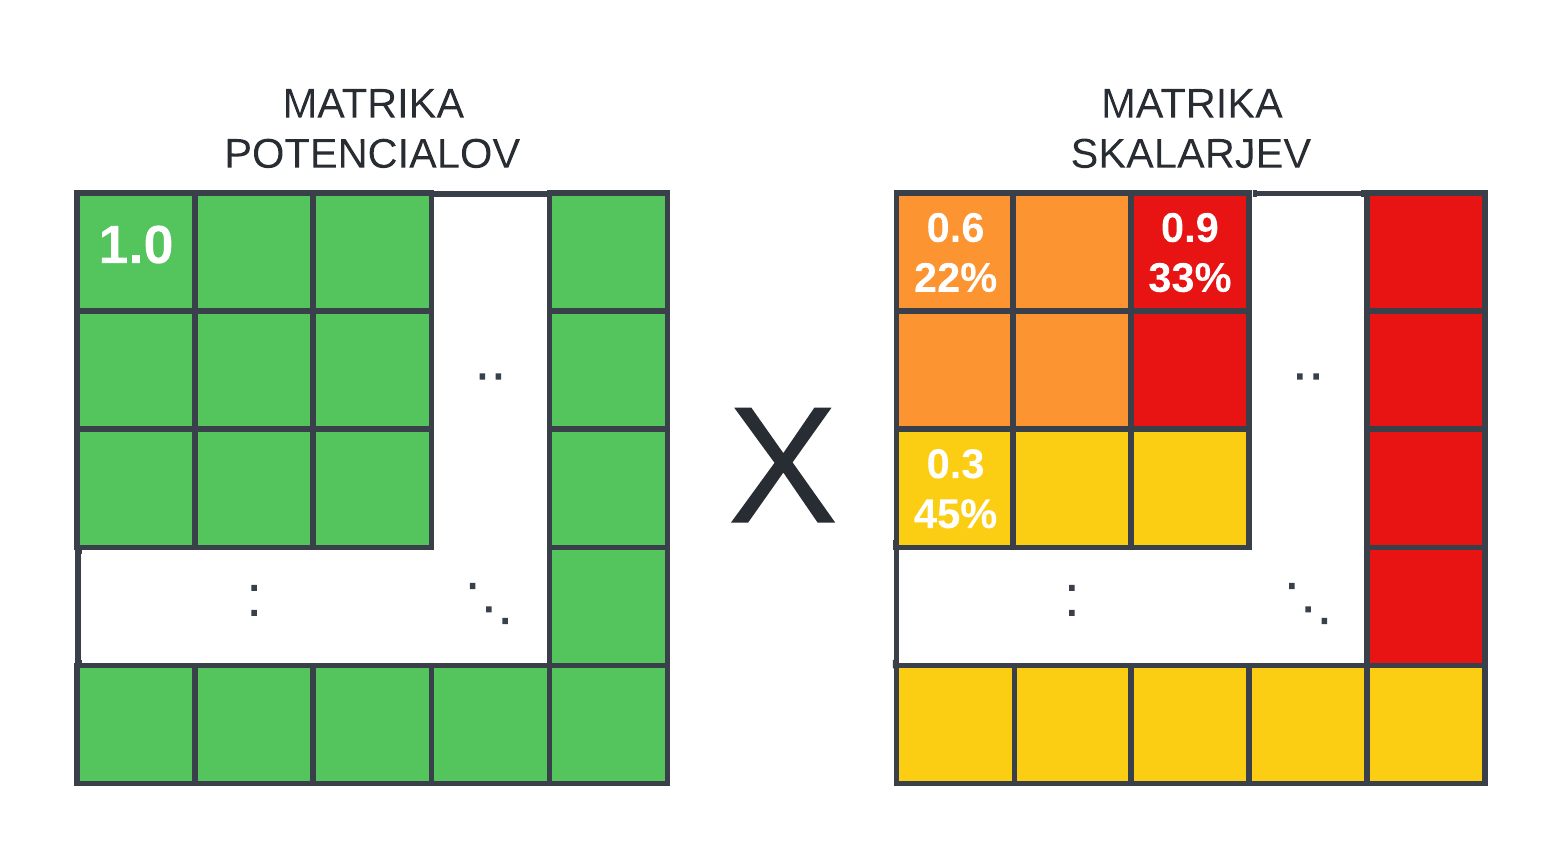
\includegraphics[width=110mm]{Slike/Območno množenje.png}
    \caption{Delovanje območnega množenja s skalarjem}
    \label{fig:območnoMnoženje}
\end{figure}


\subsection{Zgoščevalnik točk}
\label{zgoščevalnikTočk}

Zgoščevanje točk izvedemo po oblikovanju matrike potencialov in omogoča poljubno veliko povečanje resolucije naključno hrapave površine po izbrani dimenziji. Uporabljamo metodo bikubične interpolacije, ki nam omogoča gladke prehode ob hitrih spremembah gradienta med sosednjimi elementi v matriki potencialov.

\begin{figure}[H]
    \centering
    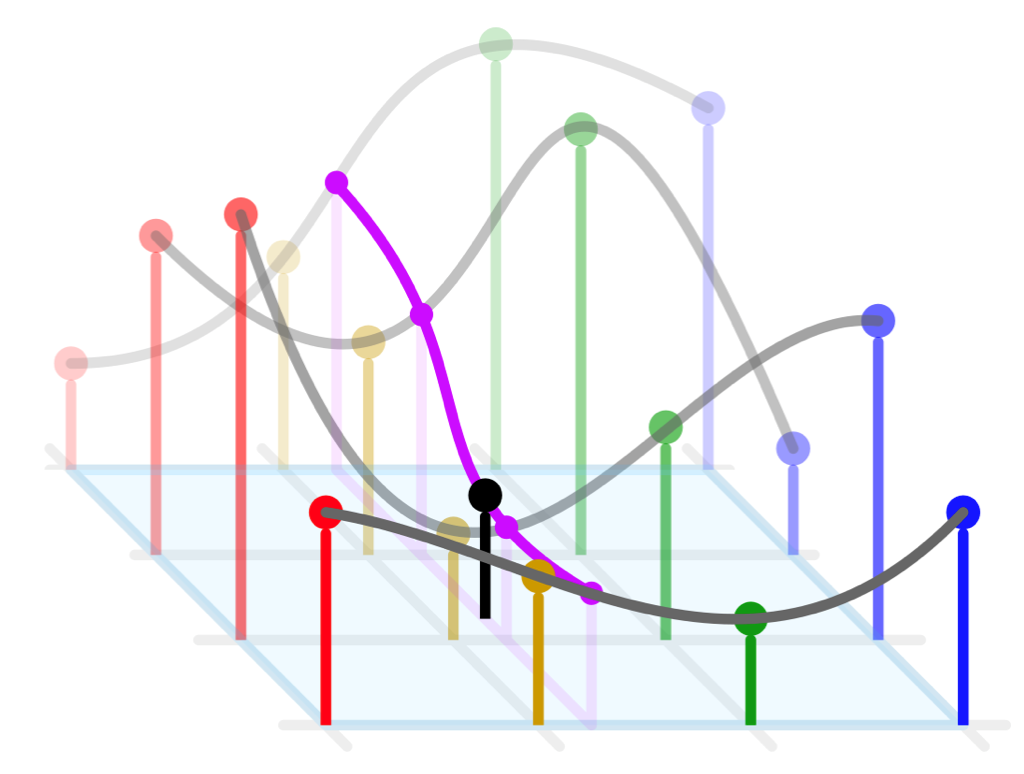
\includegraphics[width=80mm]{Slike/bikubična interpolacija.png}
    \caption{Grafična predstavitev bikubične interpolacije točk}
    \label{fig:my_label}
\end{figure}


\subsection{Izračun in prikaz parametrov generirane površine}
\label{izračunInPrikaz}

Izračun parametrov generirane površine se izvede po zgoščevalniku točk, ker se po predelavi podatkov matrika potencialov ne spreminja in je že končna. Naprej izračunamo različne hrapavosti površine:

\begin{itemize}
    \setlength\itemsep{0.1em}
    \item Povprečna hrapavost ($\bf R_a$) \footref{refnote}
    \item Efektivna hrapavost ($\bf R_q$) \footref{refnote}
    \item Maksimalna globina dolin površine ($\bf R_v$) \footref{refnote}
    \item Maksimalna višina vrhov površine ($\bf R_p$) \footref{refnote}
    \item Maksimalna razlika med dolinami in vrhovi površine ($\bf R_z = R_v + R_p$) \footref{refnote}
\end{itemize}

Omenjene vrednosti se izračuna preko povprečnega prečnega profila (od sedaj naprej profil) generirane matrike potencialov. \cite{matlab_sr} Omenjena poenostavitev nam olajša problem, saj so izračuni hrapavosti lažji:

\begin{itemize}
    \setlength\itemsep{0.1em}
    \item Povprečna hrapavost je enaka absolutnemu povprečju profila
    \item Efektivna hrapavost je enaka standardni deviaciji profila
    \item Maksimalna globina dolin je enaka absolutni minimalni vrednosti v profilu
    \item Maksimalna višina vrhov je enaka maksimalni vrednosti v profilu
    \item Maksimalna razlika je enaka seštevku minimalne in maksimalne vrednosti v profilu
\end{itemize}

Podobno pri izračunu korelacijske dolžine predpostavimo izotropijo razmika med elementi, ki je pri naši metodi generacije matrike potencialov privzeta v primeru, da sta 2 para vhodnih parametrov enaka, \textbf{xSize} mora biti enak \textbf{ySize} ter \textbf{upscaleXSize} mora biti enak \textbf{upscaleYSize}. Omenjen izračun ima sledeče korake:


\begin{enumerate}
    \setlength\itemsep{0.1em}
    \item Inicializiramo seznam enake velikosti, kot je matrika potencialov, ter v njega vpišemo ničle 
    \footnotetext[1]{Omenjene vrednosti so poračunane za površino $S_x$, a označene z $R_x$ v programu\label{refnote}}
    \item Za vsako vrstico in stolpec v matriki izračunamo križno korelacijo z vsako sosednjo vrstico oziroma stolpcem ter seštete vrednosti prve periode križne korelacije zapišemo v seznam
    \item Vse vrednosti v seznamu delimo s številom vseh elementov matrike potencialov, da normaliziramo vrednosti križnih korelacij
    \item Ustvarimo števec k, ki se povečuje dokler ne najdemo prve vrednosti v seznamu normiranih križnih korelacij, ki je manjši od $e^{-1}$
    \item Izračunamo korelacijsko dolžino po sledeči formuli (matriko potencialov preimenujemo v \textit{mtrx}):\\
    
    \begin{center}
        $\xi = \left| \frac{1}{2} * ( mtrx[k-1] + mtrx[k] - 2 * mtrx[1]) \right|$ \ \ \ \ \ \ \ \ \ \ \ \ \cite{mysimlabs_cl} \cite{gwydion_cl}
    \end{center} 
    
\end{enumerate}

Po numeričnem ovrednotenju generirane naključno hrapave površine nadaljujemo s prikazom površine v grafu ter izračunom dvodimenzionalne Fourierove transformacije, ki nam prikaže možna odstopanja v visoko-frekvenčnem spektru oziroma vidimo, ali je določen kos naključno hrapave površine v realnosti neizvedljiv. Prikz omenjene površine in grafa je mogoče izklopiti v grafičnem vmesniku z gumbom.\\

\begin{figure}[H]
    \centering
    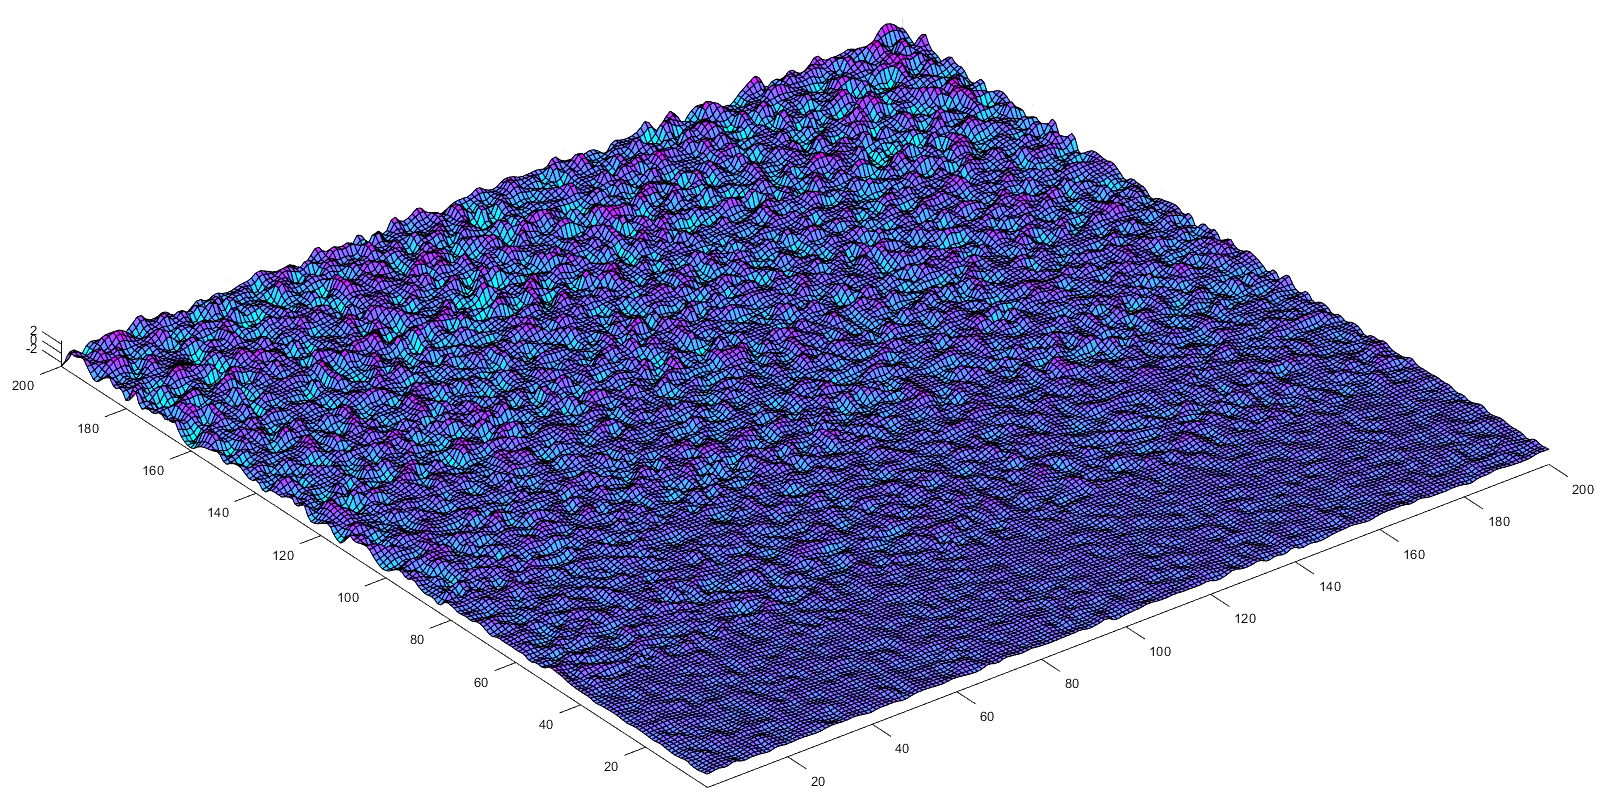
\includegraphics[width=110mm]{Slike/Noise texture.png}
    \caption{Primer raznolike naključno hrapave površine}
    \label{fig:nanohrapavaPovršina}
\end{figure}

\begin{figure}[H]
    \centering
    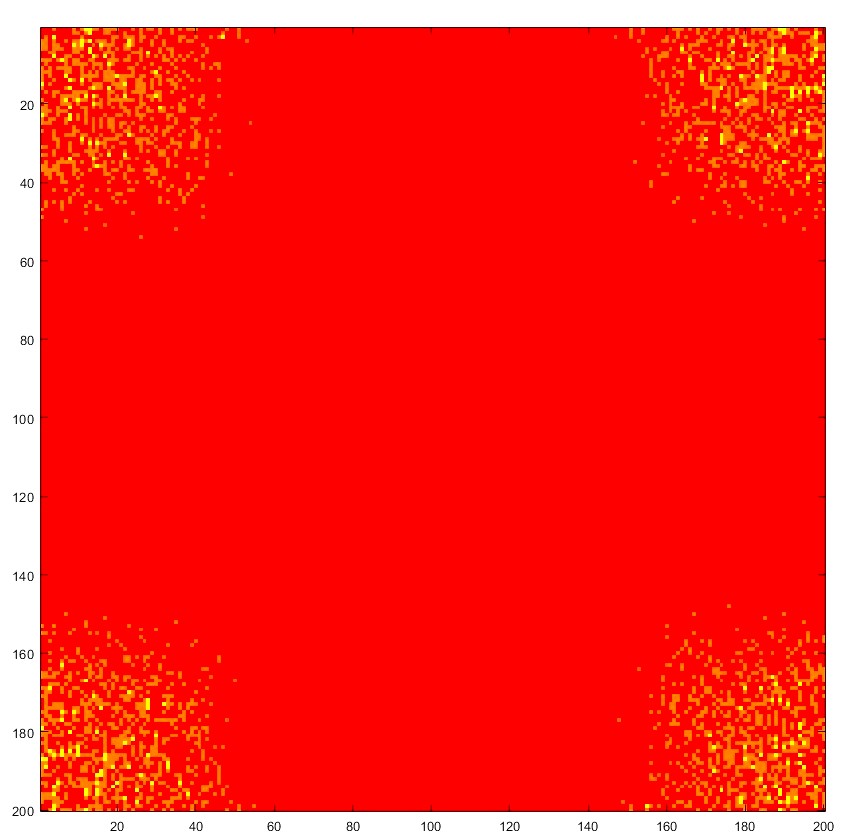
\includegraphics[width=60mm]{Slike/FFT texture.png}
    \caption{Primer dvodimenzionalne Fourierjeve transformacije naključno hrapave površine}
    \label{fig:FFTPovršine}
\end{figure}

\subsection{Zapis v besedilno datoteko}
\label{zapisVBesedilo}

Zapis v besedilno datoteko je prilagojen simulatorju CROWM, ki sprejme le-to ter jo namesti na določene spoje med materiali. Na začetku v datoteko zapišemo vseh 18 vhodnih parametrov ločenih po kategorijah ter zaporedju izvajanja. Sledijo izračunane numerične vrednosti hrapavosti in korelacijske dolžine, nato pa dodamo ključno besedilno prelomnico in vrednosti, ki določijo začetek zapisa fizičnih dimenzij naključno hrapave površine v mikrometrih ter korak vzorčenja le-te (Vhodni parametri: \textbf{xUm}, \textbf{yUm}, \textbf{d\_RT}). Na koncu sledi še zapis celotne matrike potencialov, ki jo simulator pretvori v zvezno površino ter jo vzorči.\\

\begin{figure}[H]
    \vspace{-15pt}
    \centering
    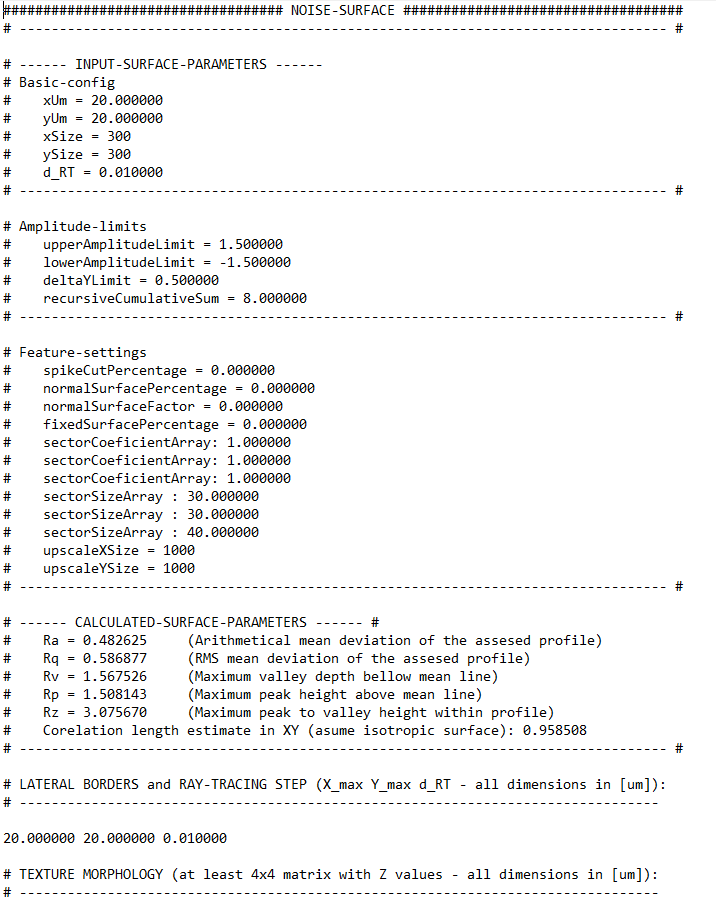
\includegraphics[width=130mm, height=139mm, trim={0 17 15 1}, clip]{Slike/vhodna datoteka.png}
    \caption{Primer izhodne datoteke generatorja naključno hrapavih površin}
    \label{fig:my_label}
\end{figure}

\clearpage

\section{Primeri generiranih naključno hrapavih površin}

\begin{figure}[htp!]
\centering

\begin{tabular}{c}
  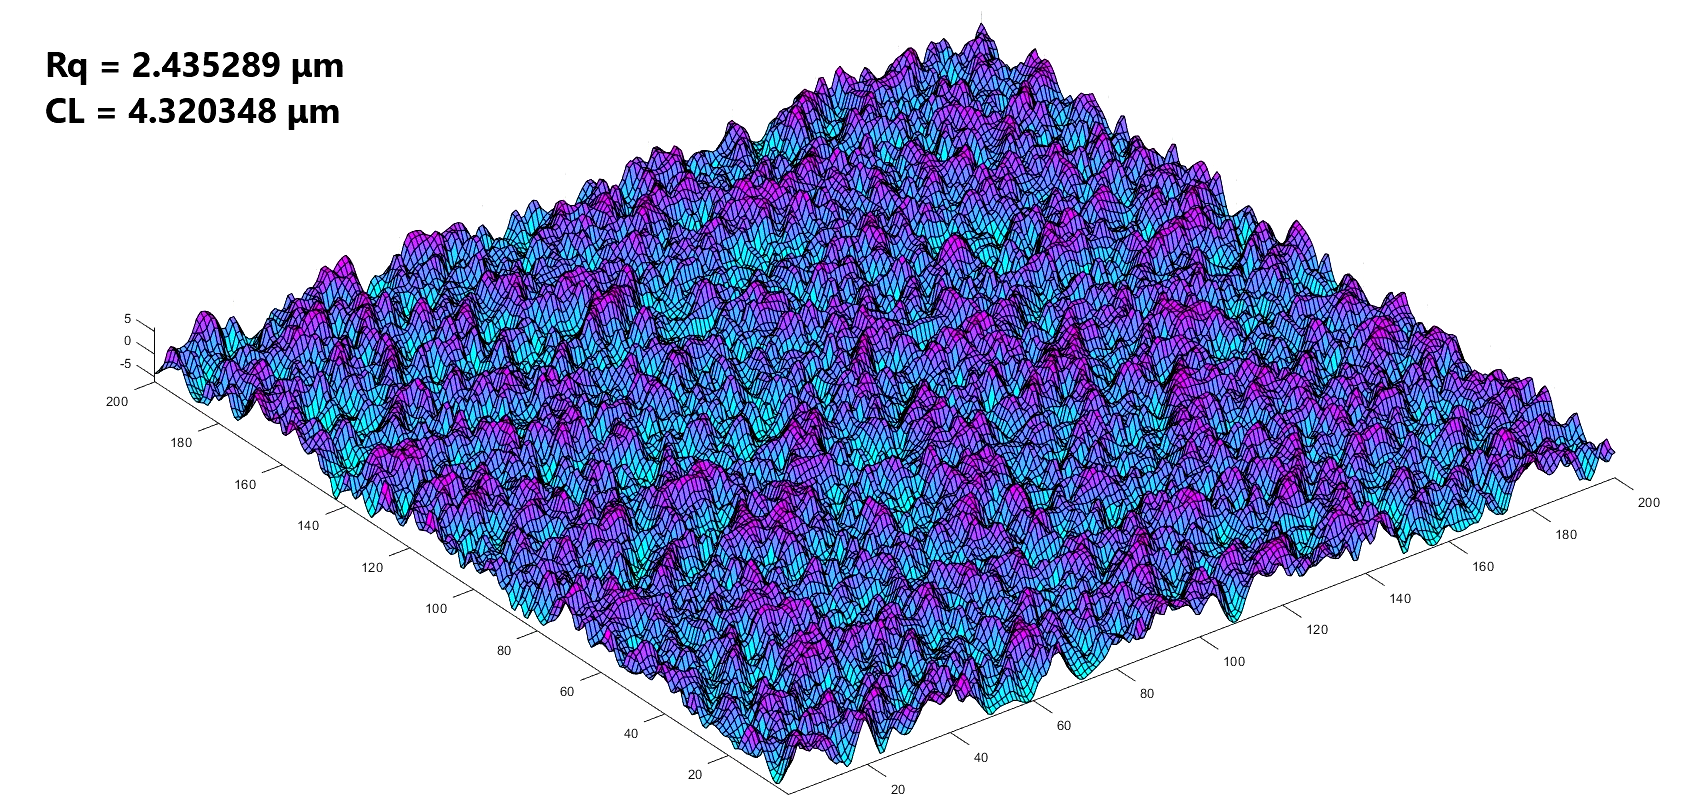
\includegraphics[height=55mm]{Slike/RQ2-5.png} \\
  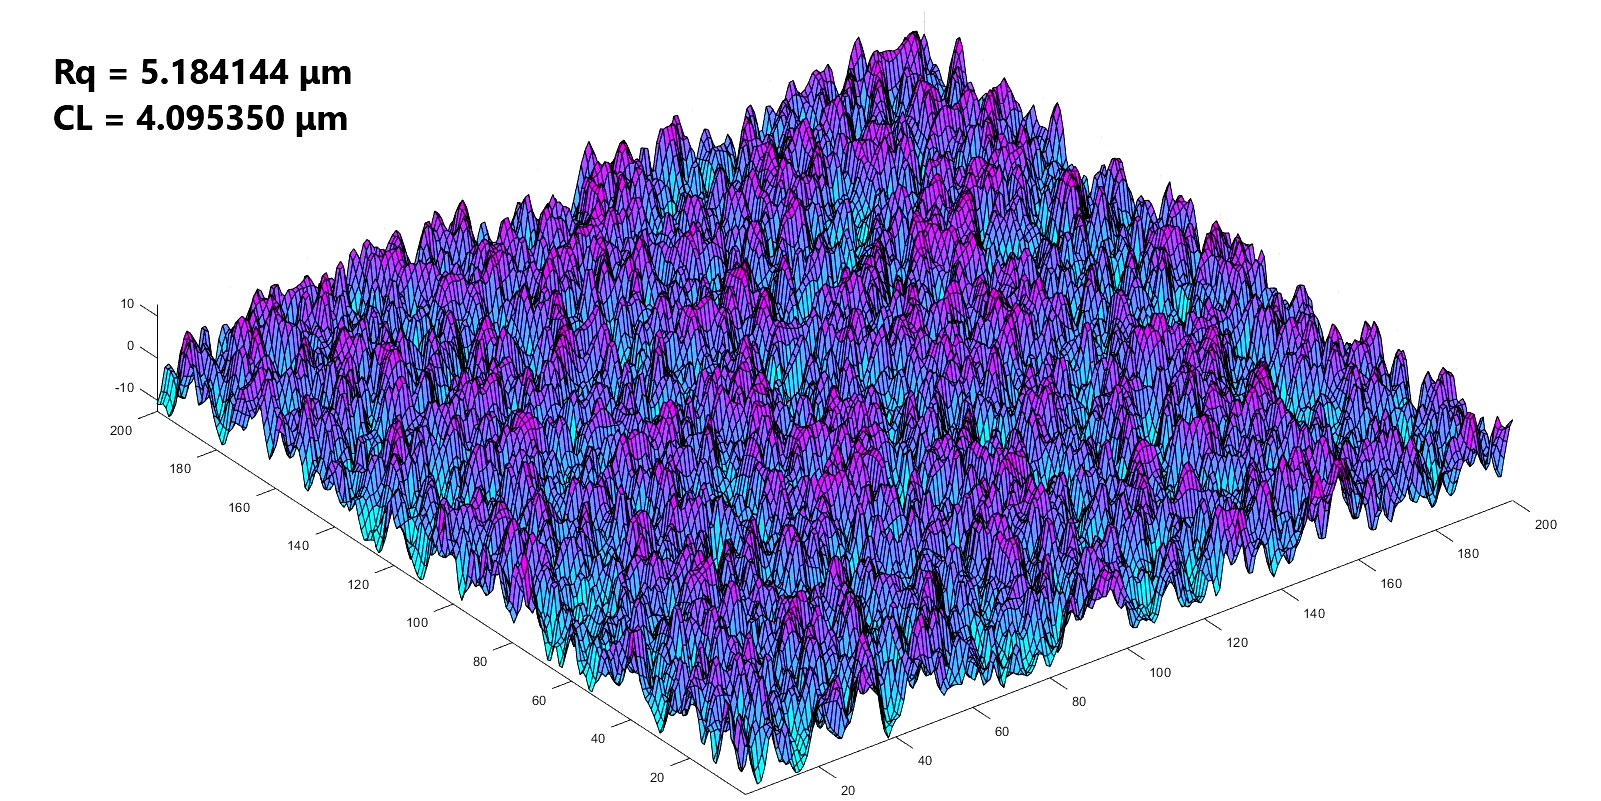
\includegraphics[height=58mm]{Slike/RQ5.png} \\
  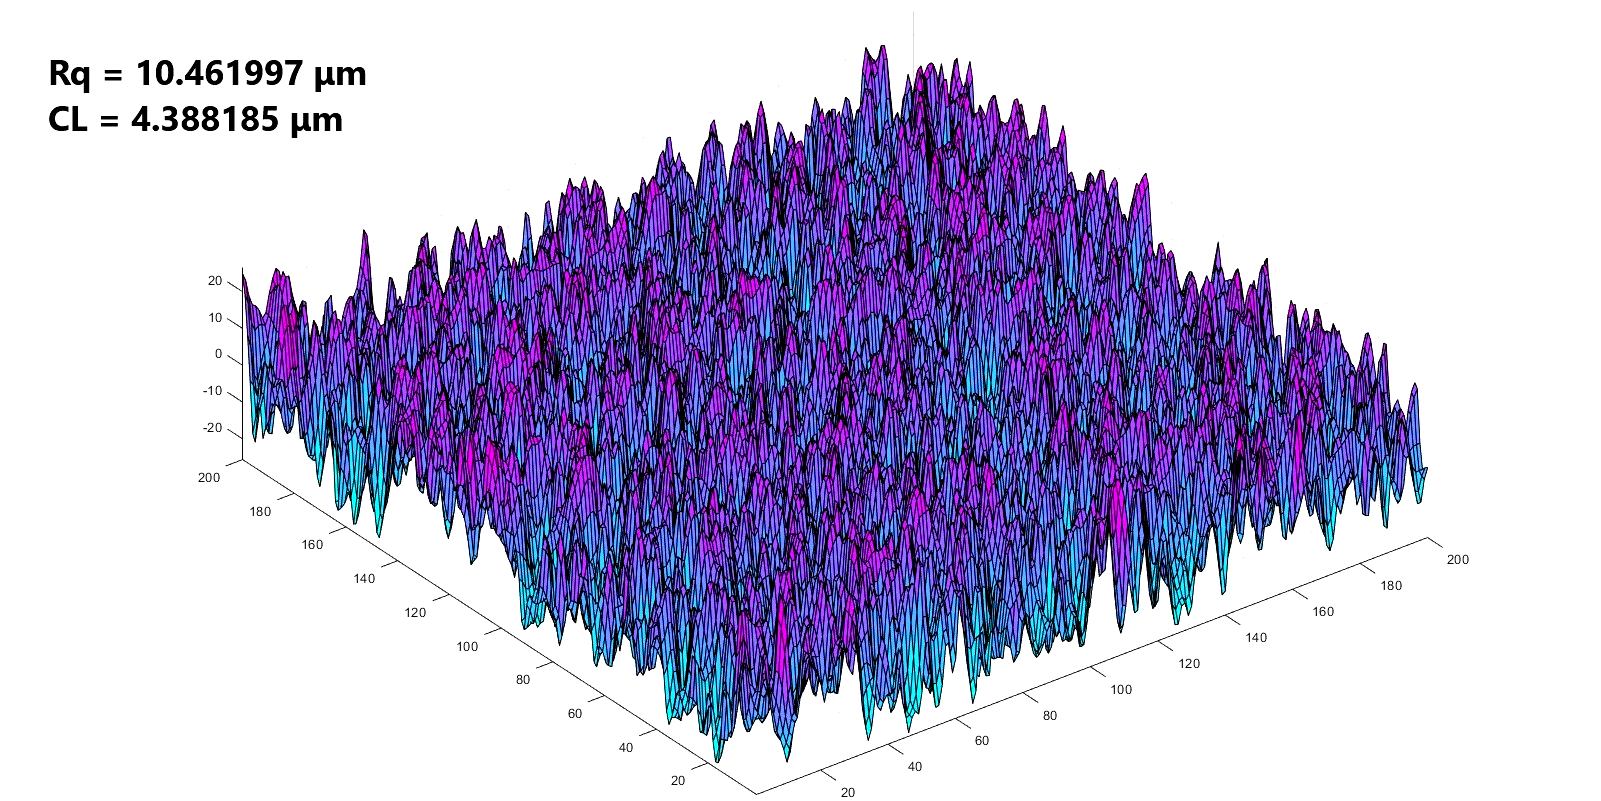
\includegraphics[height=65mm]{Slike/RQ10.png} \\
\end{tabular}

\caption{Primeri naključno hrapavih površin s pripadajočo efektivno hrapavostjo in korelacijsko dolžino}
\end{figure}

\begin{figure}[htp!]
\centering

\begin{tabular}{c}
  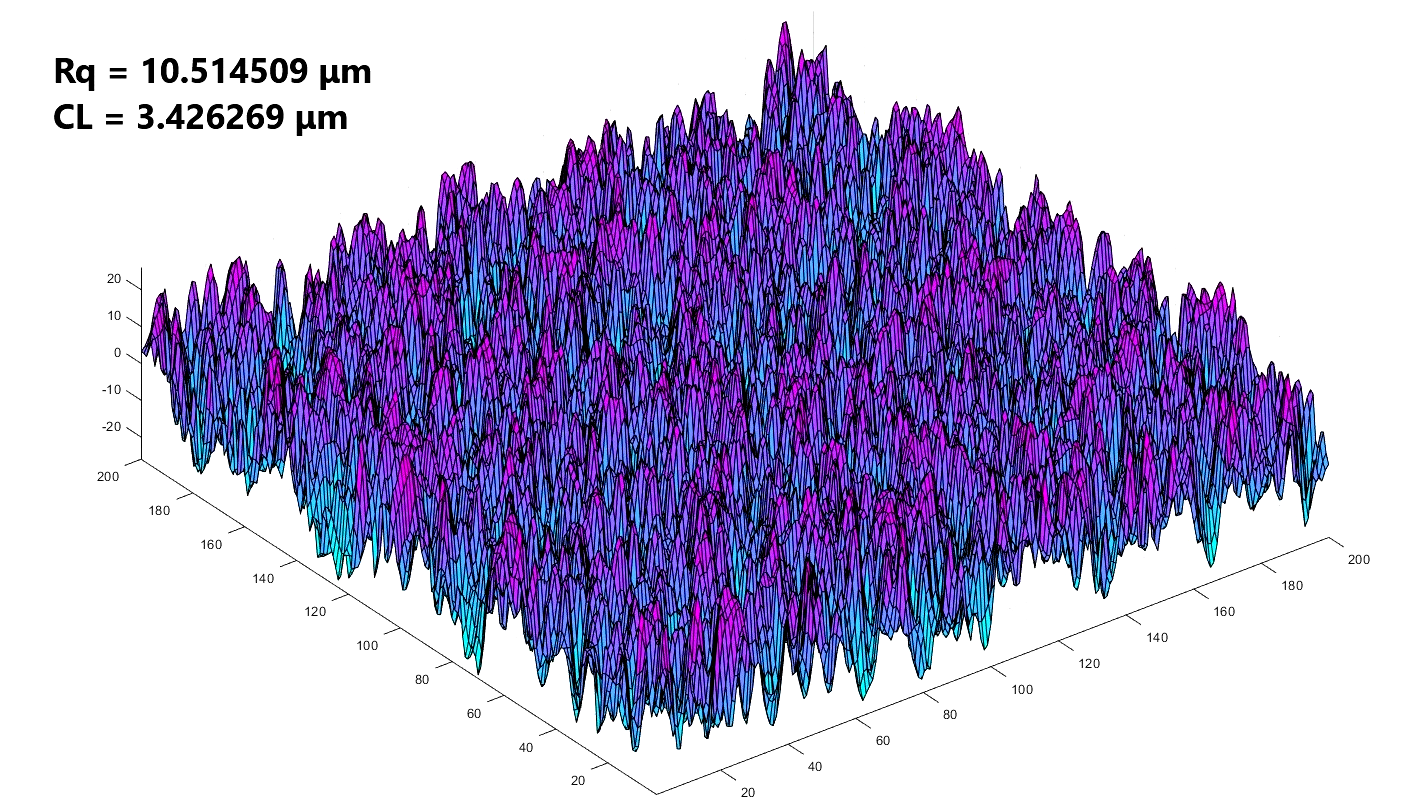
\includegraphics[width=114mm]{Slike/CL3.png} \\
  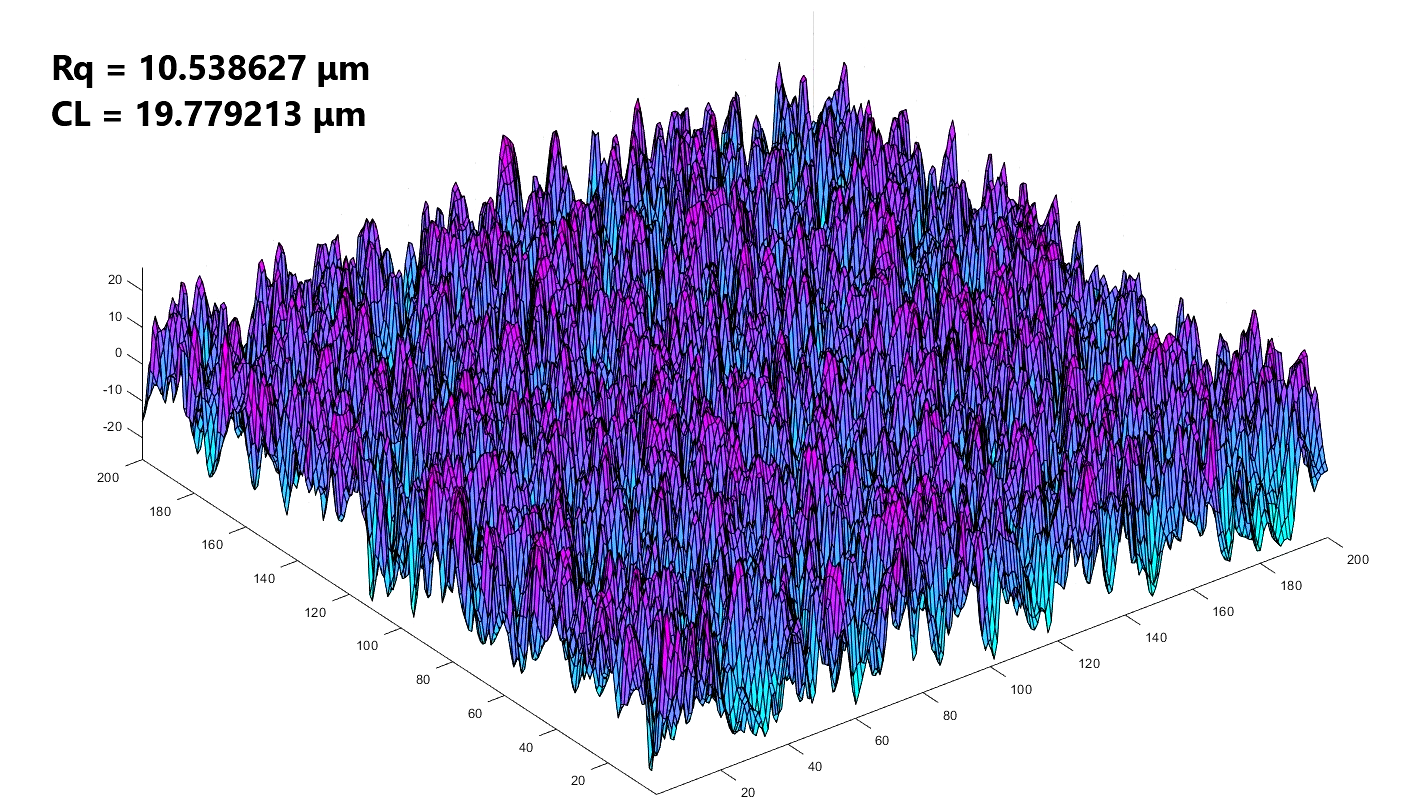
\includegraphics[width=114mm]{Slike/CL19.png} \\
  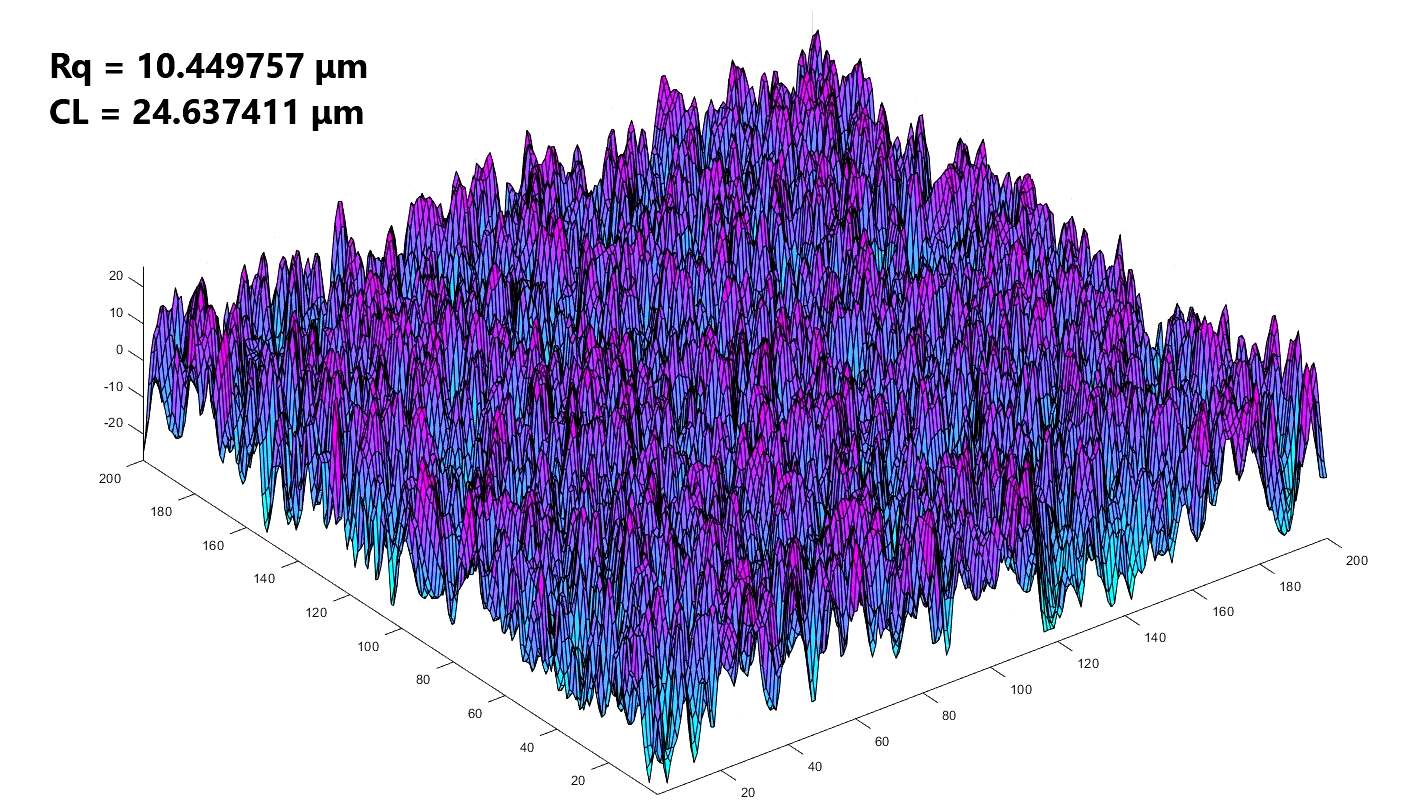
\includegraphics[width=114mm]{Slike/CL24.png} \\
\end{tabular}

\caption{Primeri naključno hrapavih površin s pripadajočo efektivno hrapavostjo in korelacijsko dolžino}
\end{figure}


\chapter{Avtomatizacija procesa}

Avtomatizacija procesa se nanaša na zaporedno izvajanje različnih simulacij v CROWM-u. Program je napisan v skriptnem jeziku PowerShell, ker nam omogoča izkoristek celotnega operacijskega sistema ter je standardno napisan za različne operacijske sisteme. Za izvedbo ene simulacije CROWM zahteva sledeči dve vhodni datoteki:

\begin{itemize}
    \setlength\itemsep{0.1em}
    \item Naključno hrapavo površino primernega formata (generacija opisana v prejšnjem poglavju)
    \item Vhodno nastavitveno datoteko za simulator CROWM
\end{itemize}

Prav tako je potrebno na koncu pridobljene rezultate simulacij ovrednotiti ter jih predstaviti v primernem formatu oziroma grafu. V tem primeru relevantne rezultate zberemo na koncu vsake izvedene simulacije ter ob zaključku vseh vrst simulacij primerjamo, ali se relevantni rezultati ujemajo z željenimi v določenem območju napake. 

\noindent Generalno je avtomatizacijski proces razdeljen na 3 dele:

\begin{itemize}
    \setlength\itemsep{0.1em}
    \item \hyperref[generatorVhodneDatoteke]{Generator vhodne nastavitvene datoteke za simulator CROWM}
    \item \hyperref[zaporednoIzvajanje]{Zaporedno izvajanje simulacij}
    \item \hyperref[zbiranjeRezultatov]{Zbiranje relevantnih rezultatov simulacij}
\end{itemize}


\section{Generator vhodne nastavitvene datoteke za simulator CROWM}
\label{generatorVhodneDatoteke}

Generator vhodne nastavitvene datoteke za simulator CROWM (od sedaj naprej generator vhodne datoteke) je bil izdelan z namenom, da lahko poleg iteriranja preko različnih naključno hrapavih površin omogočimo tudi iteracijo preko različnih nastavitev simulatorja in posledično izberemo najbolj optimalno kombinacijo parametrov. V našem primeru iščemo zadovoljivo resolucijo rezultatov ob primernem času izvajanja simulacij. Prav tako nam omenjena metoda omogoči statistično ovrednotenje raznolikosti pridobljenih rezultatov. 

\noindent Generator vhodne datoteke je sestavljen iz 3 delov:

\begin{itemize}
    \setlength\itemsep{0.1em}
    \item Vstavljalnik ključnih besedilnih prelomnic
    \item Vstavljalnik numeričnih nastavitev
    \item Vstavljalnik nastavitvenih seznamov
\end{itemize}

Generator vhodne datoteke predpostavi vnaprej definirano besedilno strukturo besedilne datoteke ter jo samostojno generira in poljubno prilagaja glede na vhodne parametre.

Vstavljalnik ključnih besedilnih prelomnic deluje preko vstavljanja prelomnic na izbrane vrstice v besedilni datoteki. Vstavljalnik numeričnih vrednosti iz nastavljenega besedilnega seznama nastavitev teče po korespondenčnih vrsticah in s konstantnim odmikom 40 presledkov vpisuje numerične vrednosti izbranih nastavitev. Vstavljalnik nastavitvenih seznamov najprej zapiše ključno prelomnico za začetek seznamske nastavitve ter v naslednje vrstice zapiše elemente iz nastavitvenega seznama.


\section{Zaporedno izvajanje simulacij}
\label{zaporednoIzvajanje}

Zaporedno izvajanje simulacij je izvedeno iterativno čez različne nastavitve generatorja naključno hrapavih površin in vhodnih nastavitev simulatorja CROWM. Iteriramo lahko čez 18 vhodnih parametrov generatorja naključno hrapavih površin ter 34 nastvitev simulatorja CROWM. Edina omejitev zaporednega izvajanja simulacij je, da lahko simuliramo samo določen tip zgradbe strukture materialov, v praksi samo en tip zgradbe materialov sončne celice naenkrat. Ob vsaki iteraciji se premaknemo globje v rekurzivno strukturo programa, zato je potrebno variacijo različnih parametrov temu prilagoditi, da ne presežemo največje globine rekurzije, ki je omejena s strojno in programsko opremo. 


\section{Zbiranje relevantnih rezultatov simulacij}
\label{zbiranjeRezultatov}

Zbiranje relevantnih rezultatov simulacij omogoča agregacijo pomembnih izhodnih podatkov. Zbiranje relevantnih rezultatov simulacij poteka na dveh mestih v programu:
\begin{itemize}
    \setlength\itemsep{0.1em}
    \item Na koncu vsake izvedene simulacije
    \item Na koncu vseh izvedenih simulacij
\end{itemize}

Na koncu vsake izvedene simulacije v besedilno datoteko zapišemo sledeče podatke v obliki preglednice:
\begin{itemize}
    \setlength\itemsep{0.1em}
    \item Zaporedno številko simulacije (\textbf{i})
    \item Število žarkov ($\bf N_{rays}$)
    \item Natančnost sledenja žarkov ($\bf RT_{precision}$)
    \item Efektivno hrapavost ($\bf R_q$)
    \item Korelacijsko dolžino ($\boldsymbol{\xi}$)
    \item Seznam vrednosti kratkostičnih tokov ($\bf J_{sc}$)
\end{itemize}

Omenjeni podatki so relevantni, saj iz štirih vhodnih parametrov (dva izhodna parametra iz generatorja naključno hrapavih površin ter dva vhodna parametra iz simulatorja CROWM) dobimo en izhodni seznam, ki ga ovrednotimo za vsako kombinacijo štirih vhodnih parametrov in dobimo želeno odvisnost vpliva naključno hrapave površine na izbrano strukturo materialov v sončni celici ter posledično njeno učinkovitost. \\

\begin{figure}[h]
    \centering
    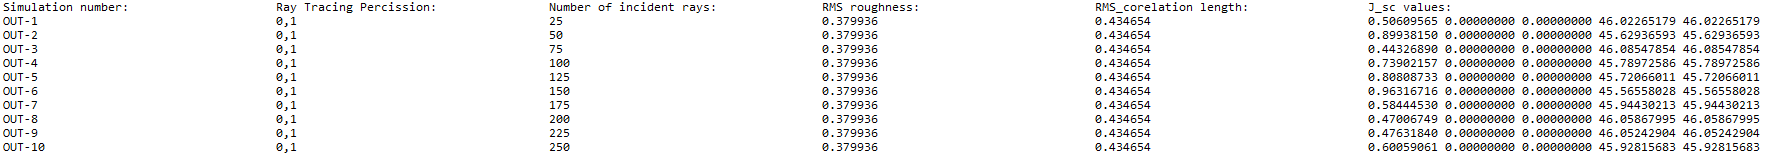
\includegraphics[width=150mm, height=25mm]{Slike/izhodna tabela.png}
    \caption{Primer izhodne besedilne datoteke}
    \label{fig:my_label}
\end{figure}


\chapter{Analiza rezultatov}

Za analizo in vizualizacijo rezultatov smo uporabili Microsoft Excel ter MATLAB, za preverbo raznolikosti podatkov pa programski jezik Python. Med relevantne podatke, ki smo jih izbrali, spadajo vhodni parametri simulatorja CROWM ter izhodni parametri generatorja naključno hrapavih površin (opisani v poglavju \ref{zbiranjeRezultatov}). Vse simulacije so uporabljale naključno hrapave površine s konstantno velikostjo generirane matrike potencialov 300x300 točk (\textbf{xSize}, \textbf{ySize}) ter zgostitvijo točk na 1000x1000 točk (\textbf{upscaleXSize}, \textbf{upscxaleYSize}). 

Simulacije, ki zavzemajo poglavja \ref{kalibSim} in \ref{izolStiki} so bile izvedene na izoliranih spojih zrak-silicij in silicij-zrak. Za vsako množico omenjenih simulacij se je izdelalo več različnih grafov za prepustnost, odbojnost ter pod pogojem, da je smiselno, tudi standardno deviacijo teh dveh količin. V primeru grafov prepustnosti in odbojnosti ne moremo govoriti direktno o kratkostičnem toku temveč o integralu prepustnosti in odbojnosti, uteženim z vpadnim spektrom, ki nam podaja rezultat v obliki kratkostičnega toka. Tega si seveda v primeru izoliranega spoja ne moremo predstavljati kot dejanski tok temveč gre za delež tokovnega potenciala, ki ga nosi vpadni spekter, ki se od površine bodisi odbije bodisi prepusti ter je relevanten za nadaljnjo analizo sončnih celic. Na grafih je razvidno spreminjanje ali števila žarkov ($\bf N_{rays}$) in natančnosti sledenja zarkov ($\bf RT_{precision}$) (poglavje \ref{kalibSim}) ali efektivne hrapavosti ($\bf R_{q}$) in korelacijske dolžine ($\boldsymbol{\xi}$) (poglavje \ref{izolStiki}). Omenjene količine predstavljajo neodvisne spremenljivke v tridimezionalnih grafih prepustnosti, odbojnosti in standardne deviacije (odvisne spremenljivke). Iz omenjenih grafov je izbiranje optimalnih parametrov za kasnejše simulacije enostavnejše.


\section{Kalibracija optičnega simulatorja}
\label{kalibSim}
Kalibracija simulatorja je določila izbrana dva parametra števila žarkov ($\bf N_{rays}$) in natančnosti sledenja žarkov ($\bf RT_{precision}$). Želeli smo ugotoviti kakšna je sprememba izhodnih rezultatov simulacij ob spreminjanju izbranih dveh parametrov optičnega simulatorja ob konstantni naključno hrapavi površini. Ob generiranju konstantne naključno hrapave površine smo bili pozorni, da je le-ta posnemala realne modele piramidnih struktur, ki v procesu izdelave sončnih celic s postopkom jedkanja nastanejo na površini silicija, ter so bile njene lastnosti primerljive le-tem. Imela je sledeče lastnosti:
\begin{itemize}
    \item Povprečno hrapavost: $\bf R_{a} = 0,290026$ $\bf \boldsymbol{\mu} m$
    \item Efektivno hrapavost: $\bf R_{q} = 0,379936$ $\bf \boldsymbol{\mu} m$
    \item Maksimalno globino dolin glede na povprečje: $\bf R_{v} = 1,277139$ $\bf \boldsymbol{\mu} m$
    \item Maksimalno višino vrhov glede na povprečje: $\bf R_{p} = 1,215669$ $\bf \boldsymbol{\mu} m$
    \item Maksimalno razliko med vrhovi in dolinami: $\bf R_{z} = 2,492808$ $\bf \boldsymbol{\mu} m$
    \item Korelacijsko dolžino: $\bf \boldsymbol{\xi} = 0,434654$ $\bf \boldsymbol{\mu} m$
\end{itemize}


\subsection{Spoj zrak-silicij}

Komentarji grafov:
\begin{itemize}
    \item \underline{\hyperref[fig:pre_air_Si]{Graf prepustnosti:}} Skupna povprečna vrednost vseh simulacij je $\bf 45,87731677$ $\bf mA/cm^2$, torej lahko ob upoštevanju $\bf \pm 20\%$ celotnega razpona pridobljenih vrednosti (razlika med največjo in najmanjšo izračunano vrednostjo parametra) trdimo, da je mejna vrednost števila žarkov ($N_{rays}$) enaka \textbf{425} žarkov za vse vrednosti natančnosti sledenja žarkov.

    \item \underline{\hyperref[fig:odb_air_Si]{Graf odbojnosti:}} Skupna povprečna vrednost vseh simulacij je $\bf 0,651430666$ $\bf mA/cm^2$, torej lahko ob upoštevanju $\bf \pm 20\%$ celotnega razpona pridobljenih vrednosti (razlika med največjo in najmanjšo izračunano vrednostjo parametra) trdimo, da je mejna vrednost števila žarkov ($N_{rays}$) enaka \textbf{425} žarkov za vse vrednosti natančnosti sledenja žarkov. Omenjena vrednost je pričakovana, saj vsota odbojnosti in prepustnosti predstavlja celoten kratkostični tok skozi spoj zrak-silicij.
    
    \item \underline{\hyperref[fig:std_air_Si]{Graf standardne deviacije:}} Prikaže odvisnost spreminjanja vhodnih parametrov CROWM ter korespondenčno napako (standardno deviacijo) izhodnih vrednosti kratkostičnega toka. Opazimo lahko, da se s spreminjanjem števila žarkov ($\bf N_{rays}$) napaka zmanjšuje hitreje kot pa s spremembo natančnosti sledenja žarkov ($\bf RT_{precision}$). Opis velja za oba grafa standardnih deviacij.
\end{itemize}

\begin{figure}[H]
    \centering
    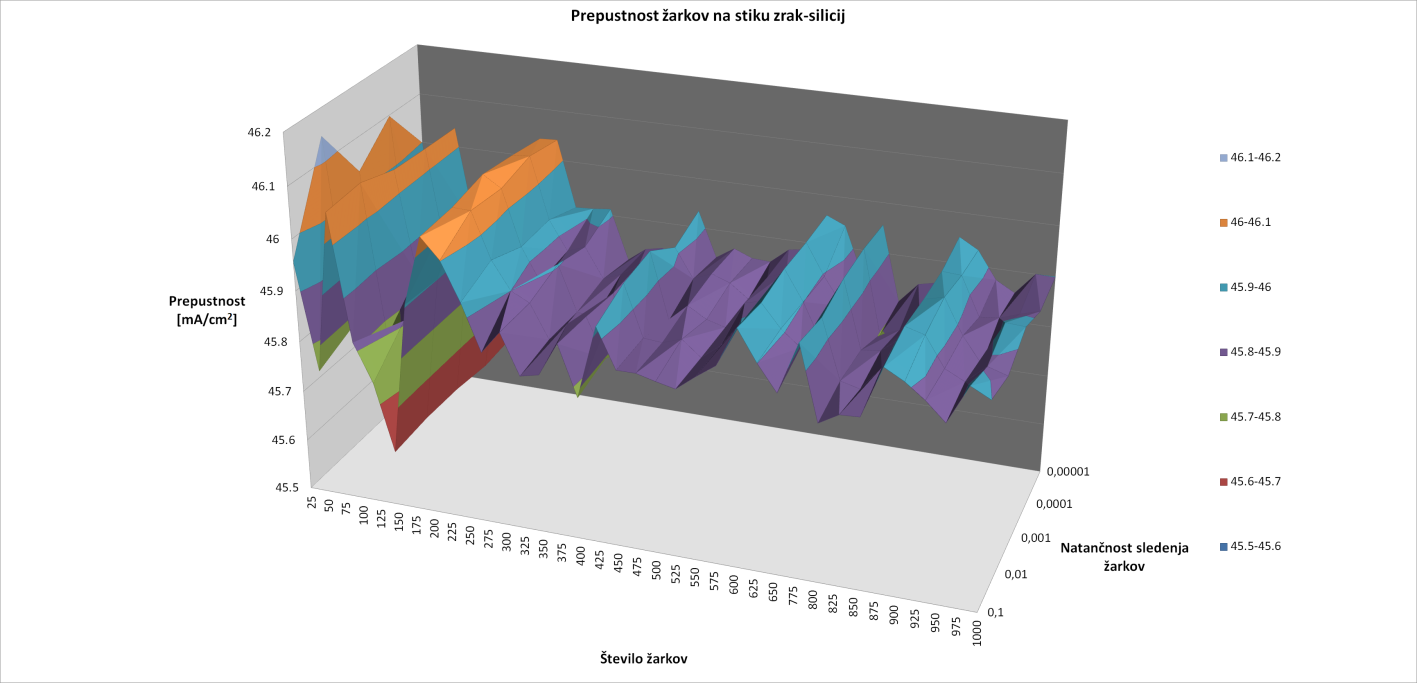
\includegraphics[trim={40 5 20 1}, clip, width=150mm]{Slike/prepustnost3D_air_Si_contTexture.png}
    \caption{Prepustnost spoja zrak-silicij (konstantna naključno hrapava površina)}
    \label{fig:pre_air_Si}
\end{figure}

\begin{figure}[h]
    \centering
    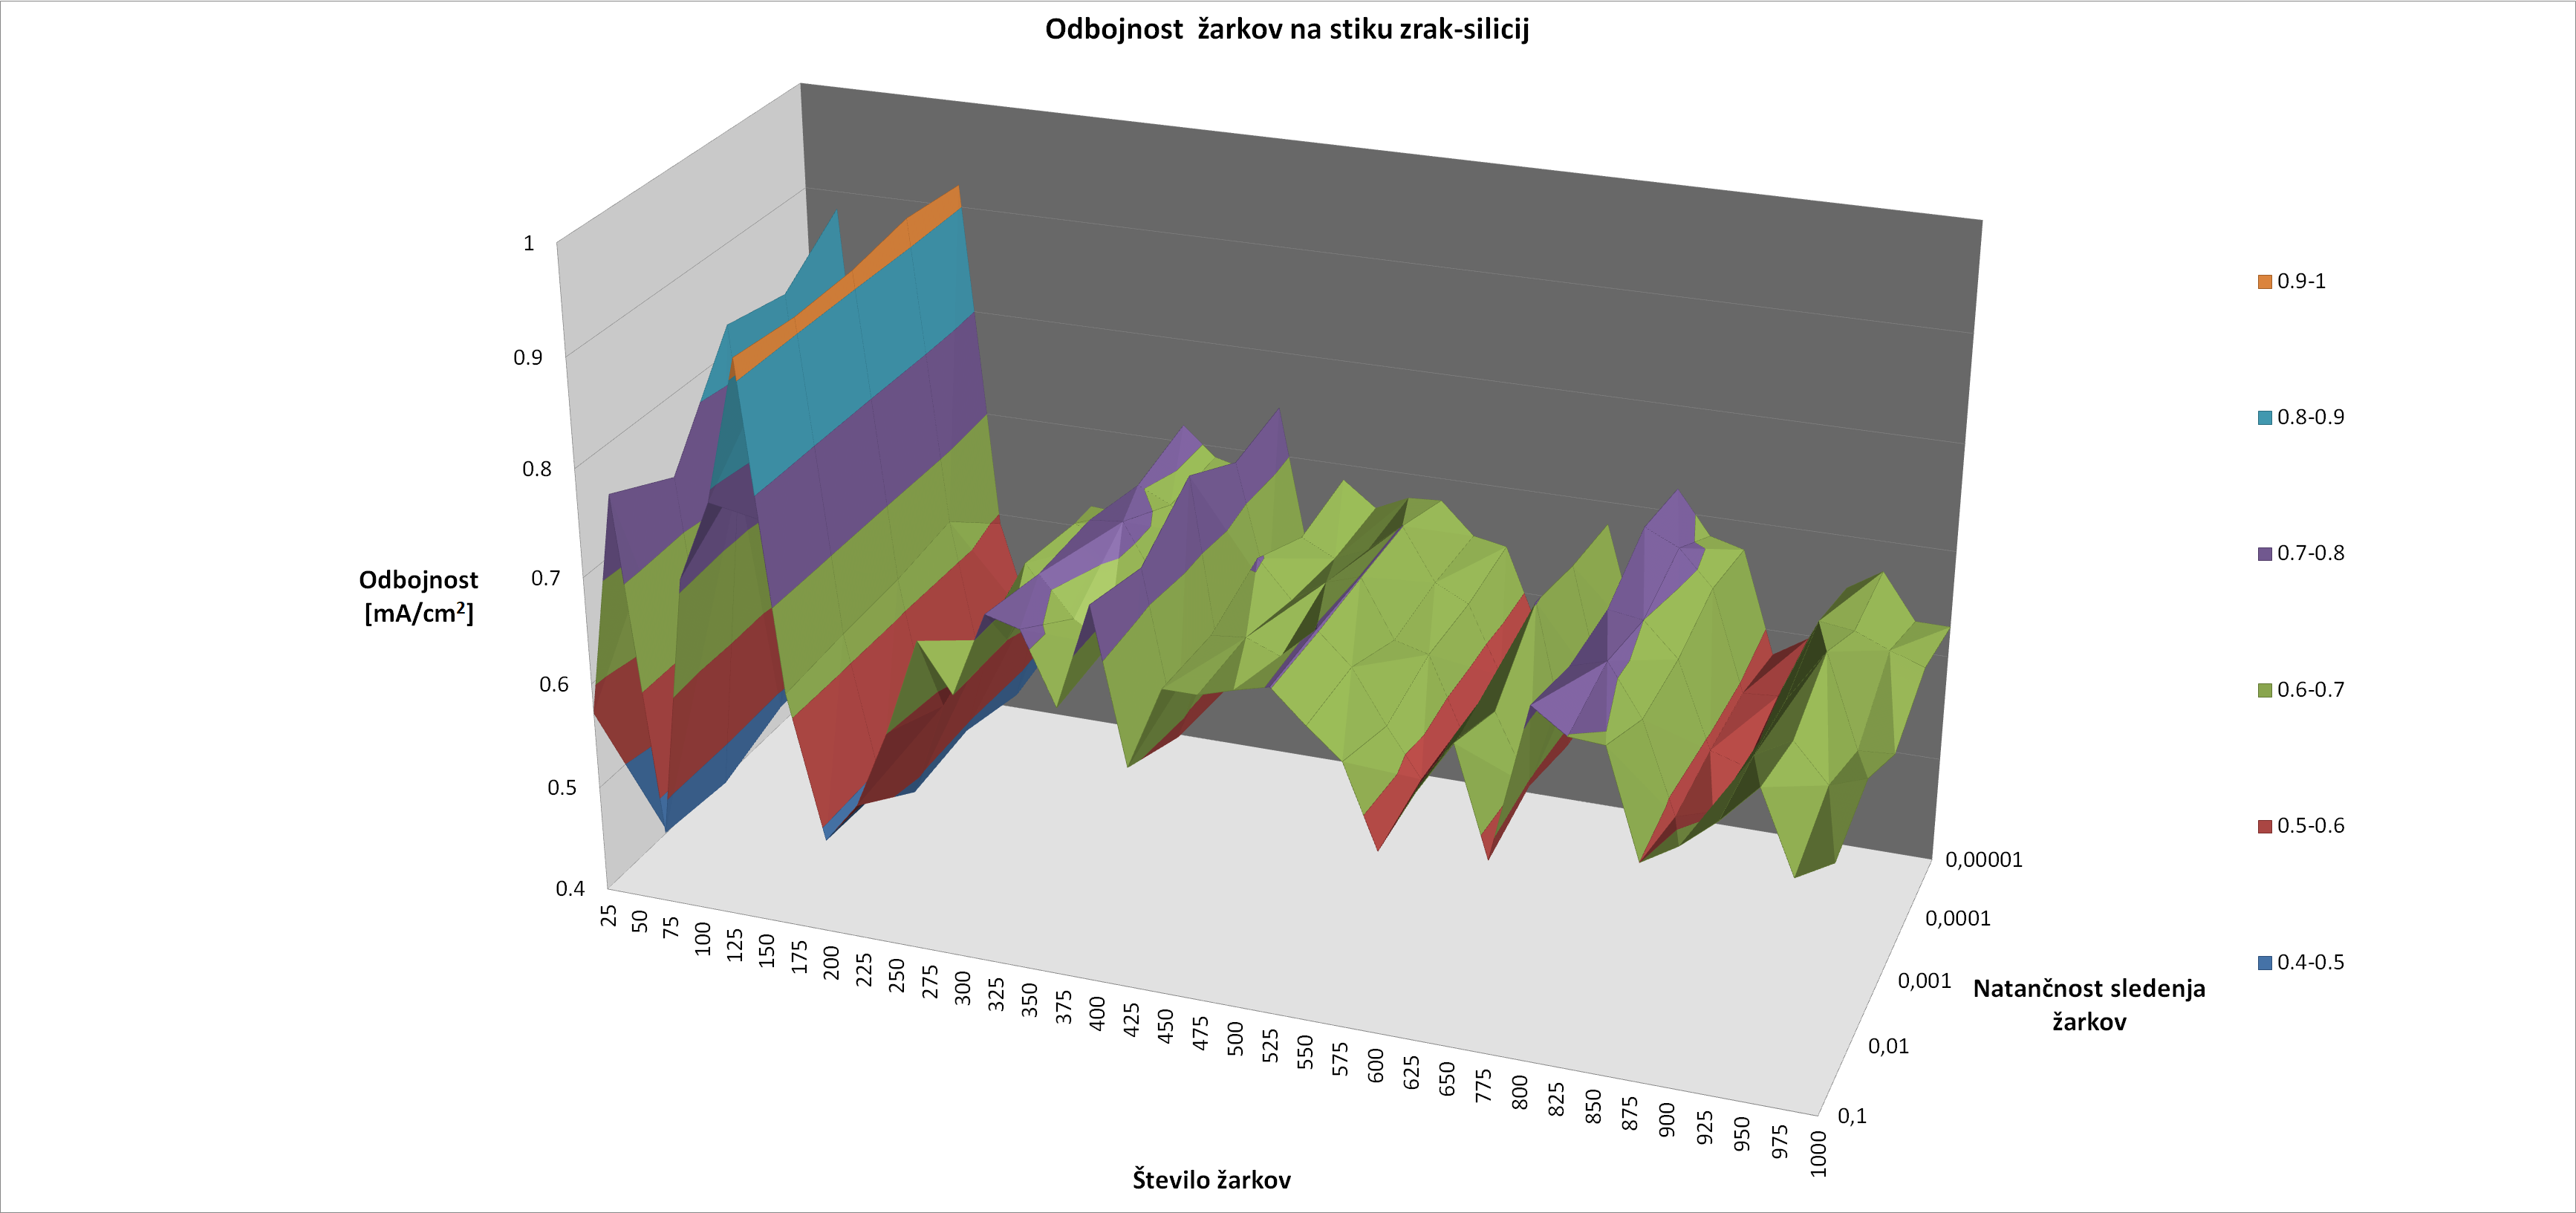
\includegraphics[trim={335 2 20 2.5}, clip, width=160mm]{Slike/odbojnost3D_air_Si_contTexture.png}
    \caption{Odbojnost spoja zrak-silicij (konstantna naključno hrapava površina)}
    \label{fig:odb_air_Si}
\end{figure}

\begin{figure}[H]
    \centering
    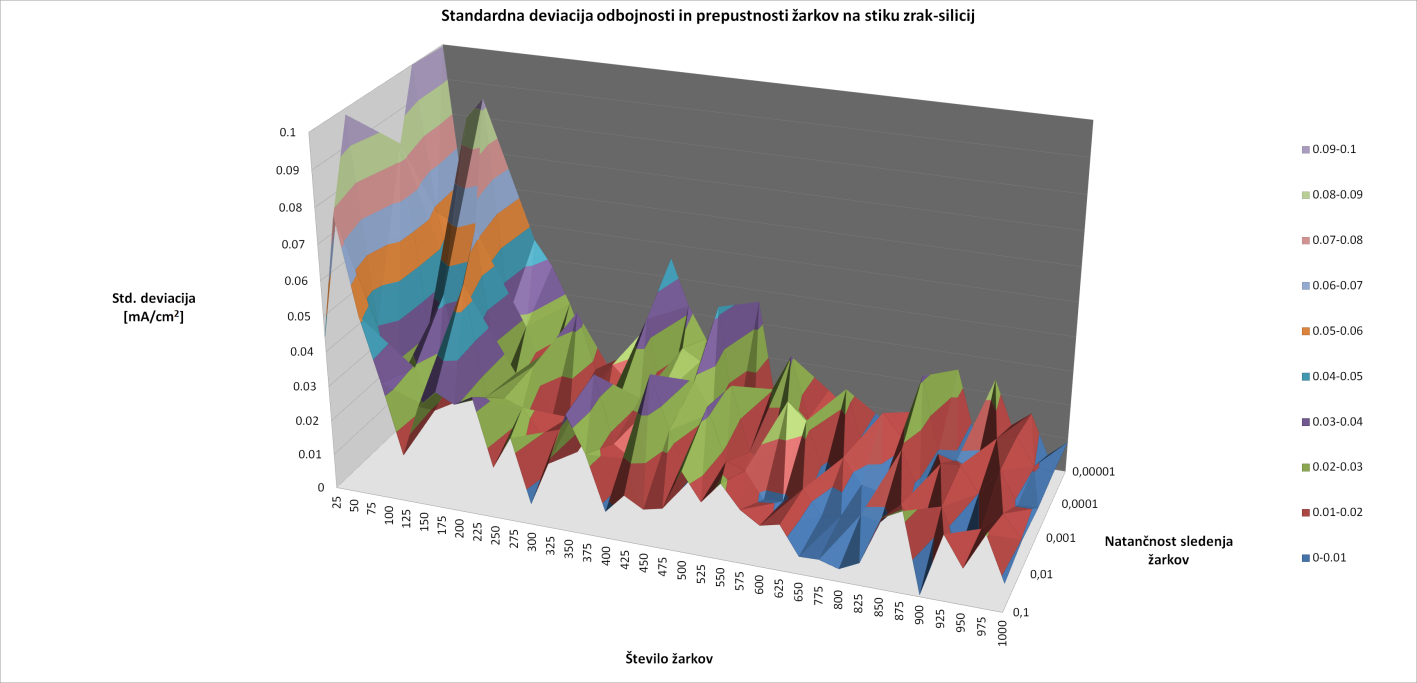
\includegraphics[trim={20 1 10 1}, clip, width=150mm]{Slike/deviacija3D_air_Si_contTexture.png}
    \caption{Standardna deviacija odbojnosti in prepustnosti spoja zrak-silicij}
    \label{fig:std_air_Si}
\end{figure}

\clearpage

\subsection{Spoj silicij-zrak}

Komentarji grafov:

\begin{itemize}
    \item \underline{\hyperref[fig:pre_Si_air]{Graf prepustnosti:}} Skupna povprečna vrednost vseh simulacij je $\bf 3,944559770$ $\bf mA/cm^2$, torej lahko ob upoštevanju $\bf \pm 20\%$ celotnega razpona pridobljenih vrednosti (razlika med največjo in najmanjšo izračunano vrednostjo parametra) trdimo, da je mejna vrednost števila žarkov ($\bf N_{rays}$) enaka \textbf{550} žarkov za vse vrednosti natančnosti sledenja žarkov.
    
    \item \underline{\hyperref[fig:odb_Si_air]{Graf odbojnosti:}} Skupna povprečna vrednost vseh simulacij je $\bf 42,584187668$ $\bf mA/cm^2$, torej lahko ob upoštevanju $\bf \pm 20\%$ celotnega razpona pridobljenih vrednosti (razlika med največjo in najmanjšo izračunano vrednostjo parametra) trdimo, da je mejna vrednost števila žarkov ($\bf N_{rays}$) enaka \textbf{550} žarkov za vse vrednosti natančnosti sledenja žarkov. Omenjena vrednost je pričakovana, saj vsota odbojnosti in prepustnosti predstavlja celoten kratkostični tok skozi spoj silicij-zrak.
    
\end{itemize}

\begin{figure}[H]
    \centering
    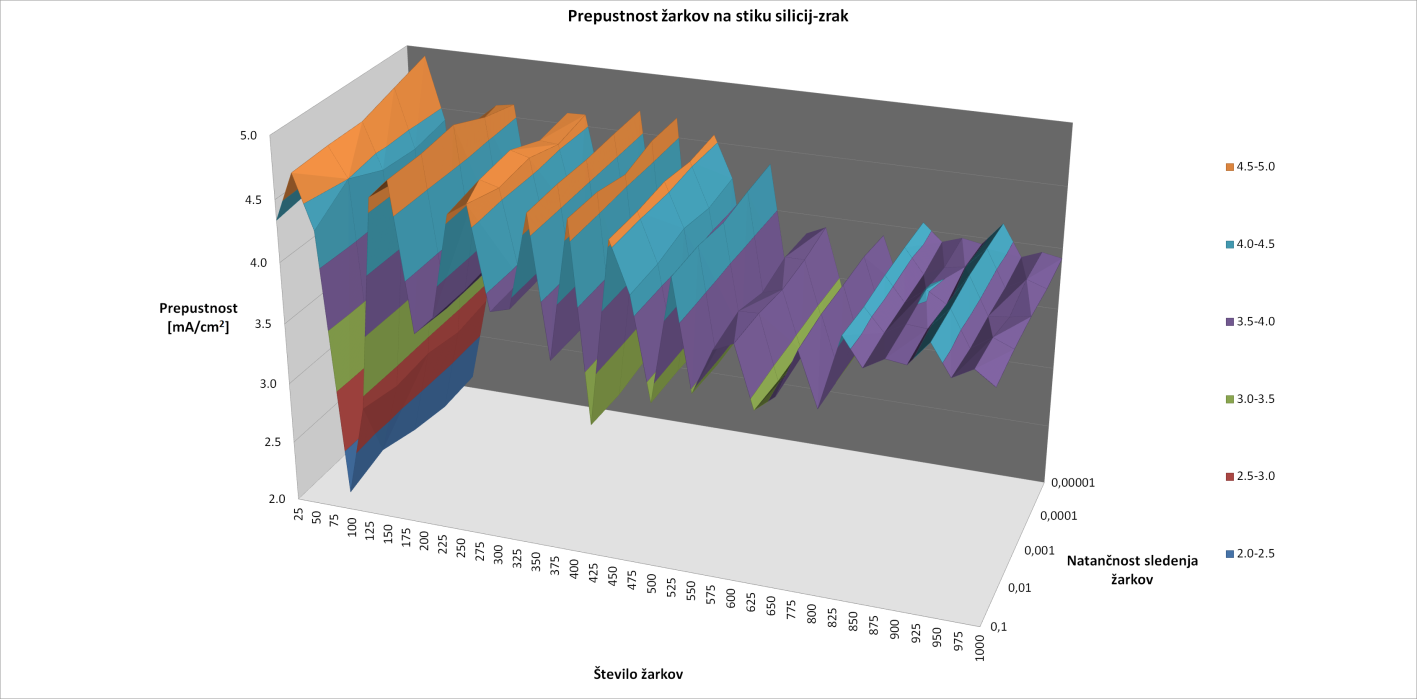
\includegraphics[trim={35 4 20 1}, clip, width=150mm]{Slike/prepustnost3D_Si_air_contTexture.png}
    \caption{Prepustnost spoja silicij-zrak (konstantna naključno hrapava površina)}
    \label{fig:pre_Si_air}
\end{figure}

\begin{figure}[H]
    \centering
    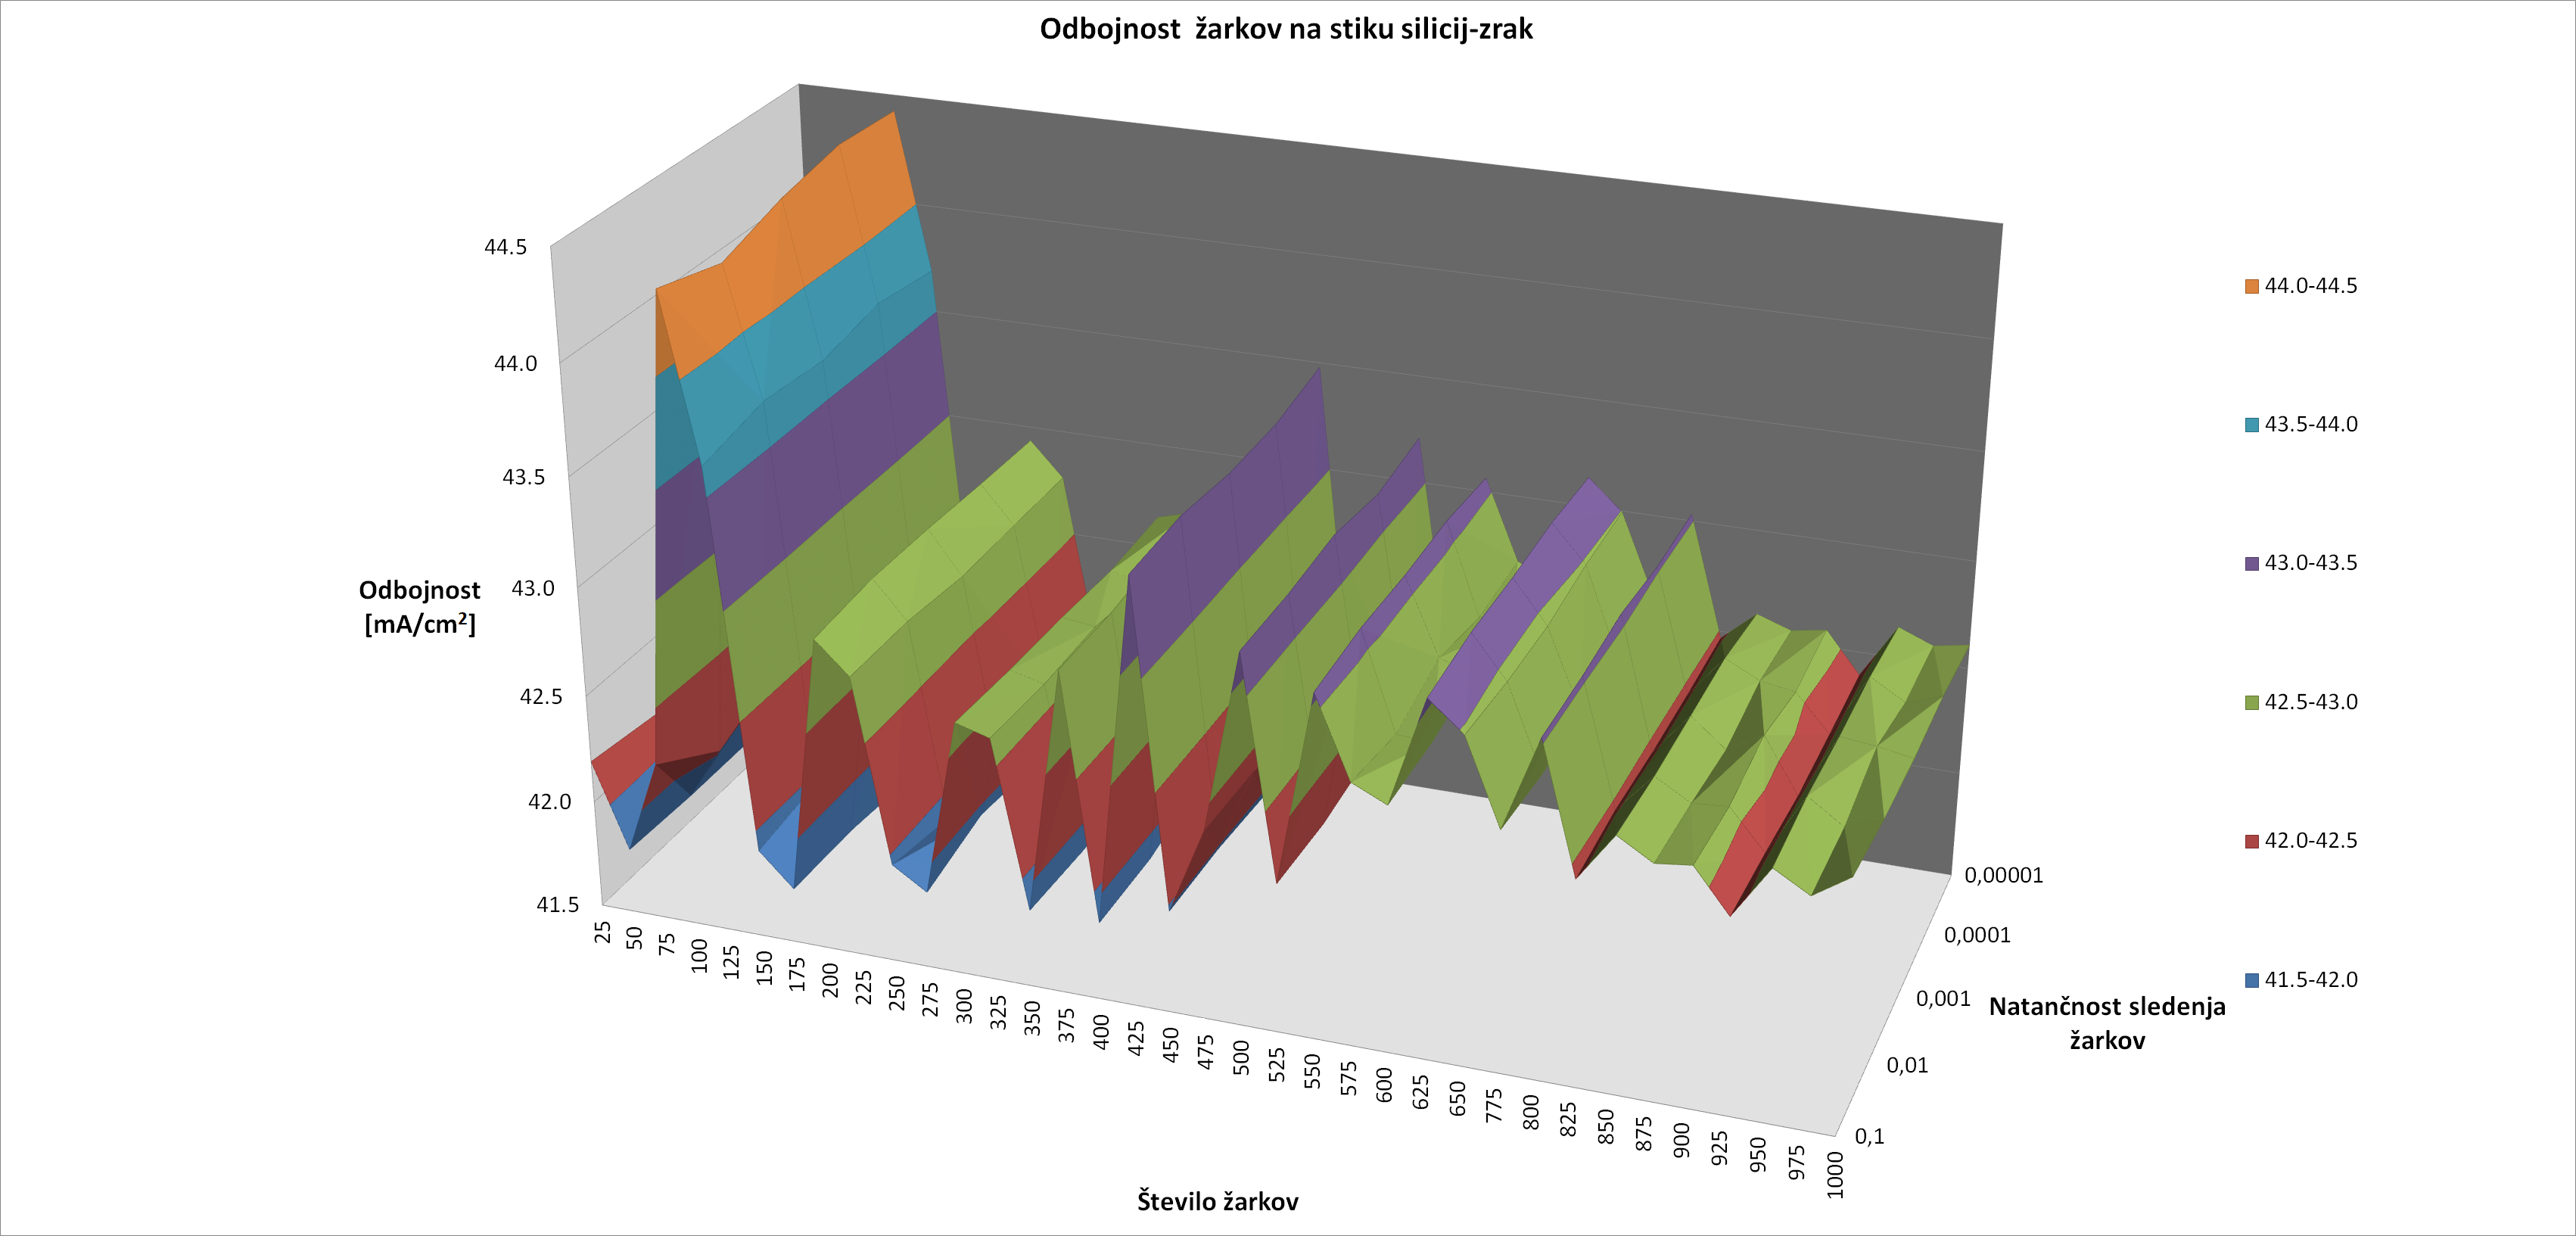
\includegraphics[trim={335 2 20 2.5}, clip, width=160mm]{Slike/odbojnost3D_Si_air_contTexture.png}
    \caption{Odbojnost spoja silicij-zrak(konstantna nakljično hrapava površina)}
    \label{fig:odb_Si_air}
\end{figure}

\begin{figure}[H]
    \centering
    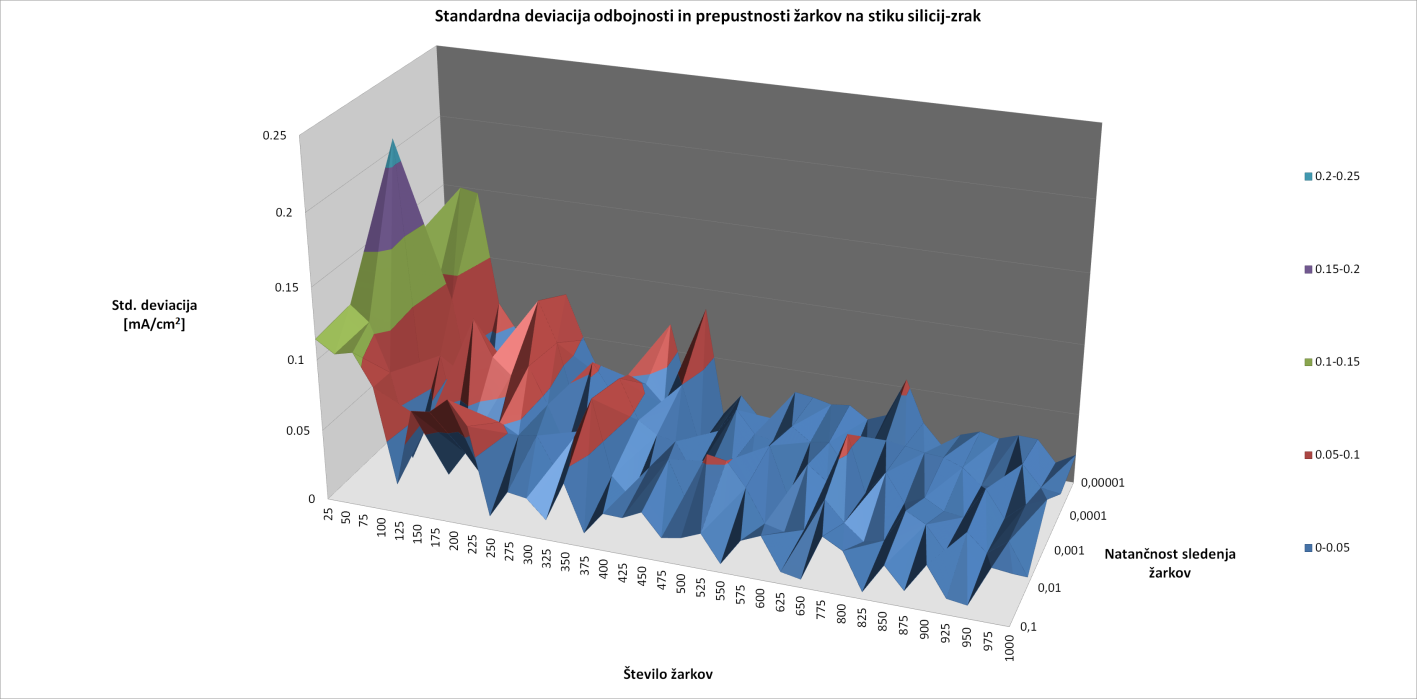
\includegraphics[trim={20 1 10 1}, clip, width=150mm]{Slike/deviacija3D_Si_air_contTexture.png}
    \caption{Standardna deviacija odbojnosti in prepustnosti spoja silicij-zrak}
    \label{fig:std_Si_air}
\end{figure}

\subsection{Preverba podatkov}

Preverbo ali verifikacijo raznolikosti podatkov smo izvedli s programskim jezikom Python ter pripadajočimi knjižnicami za statistiko. Izvedli smo Wilcoxonov preizkus vsote rangov, saj smo imeli med seboj neodvisne simulacije\ \cite{predavanje}. Iz spodnjih dveh tabel je razvidno sledeče:

\begin{itemize}
    \item \underline{\hyperref[tab:pSled]{Tabela p-vrednosti natančnosti sledenja žarkov:}} Opazimo lahko, da se s spreminjanjem natančnosti sledenja žarkov vrednosti simulacij pri enakemu številu žarkov bistveno ne razlikujejo. To pomeni, da je natančnost sledenja žarkov pri izvedbi večjega števila simulacij manj relevantna, zato lahko le-to nastavitev prilagodimo tako, da je čas simulacij krajši. Če nastavimo mejno p-vrednost pod 0,5 oziroma 50\%, ugotovimo, da le-tej zadostujeta le dve množici simulacij (v tabeli označeno z rdečo barvo) in obe na spoju zrak-silicij. Zadovoljiti hočemo obema spojema, zato je potrebno mejno p-vrednost izbrati višje (vsaj vrednost 0,807, da ustrezamo tudi spoju silicij-zrak). Na koncu smo izbrali mejno vrednost 0,9 oziroma 90\%, saj zajame štiri množice simulacij na spoju zrak-silicij ter dve množici na spoju silicij-zrak (v tabeli označeno z oranžno in rdečo barvo). Omenjeno pomeni, da lahko z 90\% verjetnostjo trdimo, da se simulacije med seboj ne bodo razlikovale. Glede na priporočila dosedanje uporabe simulatorja CROWM smo zato izbrali za natančnost sledenja žarkov vrednost $\bf 10^{-3}$.
    
    \item \underline{\hyperref[tab:pŽarek]{Tabela p-vrednosti števila žarkov:}} Tu lahko opazimo, da so p-vrednosti veliko bolj razgibane glede na natančnost sledenja žarkov. Razločimo lahko okvirne mejne pasove, kjer se p-vrednosti drastično zmanjšajo oziroma to pomeni, da so tam simulacije med seboj precej različne. V tabeli so z barvno lestvico označeni okvirni korespondenčni mejni pasovi za oba spoja. Upoštevali smo, da p-vrednost ne sme preseči mejne vrednosti 0,1 oziroma 10\%. Če poleg omenjenih p-vrednosti upoštevamo še zgornje grafe standardnih deviacij kratkostičnih tokov (grafa \ref{fig:std_air_Si}, \ref{fig:std_Si_air}), lahko ugotovimo, da je optimalna vrednost števila žarkov, ki upošteva kriterij nizke deviacije simulacij, kriterij nizke p-vrednosti ter časovno zahtevnost simulacije, okoli števila 425. Za končno vrednost smo se odločili, da število žarkov za vse naslednje simulacije nastavimo na \textbf{420}.
\end{itemize}

Končna določitev parametrov simulatorja CROWM: 

\hspace{\parindent} $\bf RT_{precision} = 10^{-3}$ , $\bf N_{rays} = 420$

\vspace{15pt}

\begin{center}

\begin{table}[h]
\begin{tabular}{|cc|cc|}
\hline
\multicolumn{2}{|c|}{\textbf{Spoj zrak-silicij}}                    & \multicolumn{2}{c|}{\textbf{Spoj silicij-zrak}}                    \\ \hline
\multicolumn{1}{|c|}{{\ul Natančnost sledenja žarkov}} & p-vrednost & \multicolumn{1}{c|}{{\ul Natančnost sledenja žarkov}} & p-vrednost \\ \hline
\multicolumn{1}{|c|}{0,1}                              &\color[HTML]{FE0000} 0,294      & \multicolumn{1}{c|}{0,1}                              & 0,970      \\ \hline
\multicolumn{1}{|c|}{0,01}                             &\color[HTML]{F56B00} 0,662      & \multicolumn{1}{c|}{0,01}                             &\color[HTML]{F56B00} 0,807      \\ \hline
\multicolumn{1}{|c|}{0,001}                            & 0,994      & \multicolumn{1}{c|}{0,001}                            &\color[HTML]{F56B00} 0,871      \\ \hline
\multicolumn{1}{|c|}{0,0001}                           &\color[HTML]{F56B00} 0,882      & \multicolumn{1}{c|}{0,0001}                           & 0,944      \\ \hline
\multicolumn{1}{|c|}{0,00001}                          &\color[HTML]{FE0000} 0,443      & \multicolumn{1}{c|}{0,00001}                          & 0,980      \\ \hline
\end{tabular}
\caption{Tabela p-vrednosti natančnosti sledenja žarkov}
\label{tab:pSled}
\end{table}

\end{center}

\vspace{-15pt}


\begin{longtable}{| p{.20\textwidth} | p{.20\textwidth} | p{.20\textwidth} | p{.20\textwidth} |}

\hline
\multicolumn{2}{|c|}{\textbf{Spoj zrak-silicij}}                              & \multicolumn{2}{c|}{\textbf{Spoj silicij-zrak}}                              \\ \hline
\multicolumn{1}{|c|}{{\ul Število žarkov}} & p-vrednost                       & \multicolumn{1}{c|}{{\ul Število žarkov}} & p-vrednost                       \\ \hline
\multicolumn{1}{|c|}{25}                   & \color[HTML]{3531FF}$1,48*10^{-9}$                     & \multicolumn{1}{c|}{25}                   & \color[HTML]{3531FF}0,000135                         \\ \hline
\multicolumn{1}{|c|}{50}                   & \color[HTML]{3531FF}$1,27*10^{-8}$                     & \multicolumn{1}{c|}{50}                   $& \color[HTML]{3531FF}1,34*10^{-7}$                     \\ \hline
\multicolumn{1}{|c|}{75}                   & \color[HTML]{3531FF}$9,27*10^{-5}$                     & \multicolumn{1}{c|}{75}                   & \color[HTML]{3531FF}0,000909                         \\ \hline
\multicolumn{1}{|c|}{100}                  & \color[HTML]{3531FF}0,00154                          & \multicolumn{1}{c|}{100}                  & \color[HTML]{3531FF}$3,89*10^{-4}$                      \\ \hline
\multicolumn{1}{|c|}{125}                  & \color[HTML]{3531FF}$1,66*10^{-8}$                     & \multicolumn{1}{c|}{125}                  & \color[HTML]{3531FF}$4,65*10^{-4}$                      \\ \hline
\multicolumn{1}{|c|}{150}                  & \color[HTML]{3531FF}$6,75*10^{-4}$                     & \multicolumn{1}{c|}{150}                  & \color[HTML]{3531FF}$3,11*10^{-10}$                      \\ \hline
\multicolumn{1}{|c|}{175}                  & \color[HTML]{3531FF}0,0776                           & \multicolumn{1}{c|}{175}                  & \color[HTML]{3531FF}$2,49*10^{-7}$                       \\ \hline
\multicolumn{1}{|c|}{200}                  & \color[HTML]{3531FF}$1,35*10^{-7}$                     & \multicolumn{1}{c|}{200}                  & \color[HTML]{3531FF}0,000361                         \\ \hline
\multicolumn{1}{|c|}{225}                  & \color[HTML]{3531FF}$3,35*10^{-7}$                     & \multicolumn{1}{c|}{225}                  & \color[HTML]{3531FF}0,00694                          \\ \hline
\multicolumn{1}{|c|}{250}                  & \color[HTML]{3531FF}0,000977                         & \multicolumn{1}{c|}{250}                  & \color[HTML]{3531FF}$1,78*10^{-10}$                    \\ \hline
\multicolumn{1}{|c|}{275}                  & \cellcolor{lime}0,943                            & \multicolumn{1}{c|}{275}                  & \color[HTML]{3531FF}$9,27*10^{-8}$                     \\ \hline
\multicolumn{1}{|c|}{300}                  & \cellcolor{lime}0,237                            & \multicolumn{1}{c|}{300}                  & \cellcolor{lime}0,226                            \\ \hline
\multicolumn{1}{|c|}{325}                  & \color[HTML]{036400}$4,12*10^{-11}$                    & \multicolumn{1}{c|}{325}                  & \cellcolor{lime}0,489                            \\ \hline
\multicolumn{1}{|c|}{350}                  & \color[HTML]{036400}0,00470                          & \multicolumn{1}{c|}{350}                  & \color[HTML]{036400}$1,80*10^{-7}$                     \\ \hline
\multicolumn{1}{|c|}{375}                  & \cellcolor{lime}0,443                            & \multicolumn{1}{c|}{375}                  & \color[HTML]{036400}0,000106                         \\ \hline
\multicolumn{1}{|c|}{400}                  & \color[HTML]{036400}$1,31*10^{-8}$                     & \multicolumn{1}{c|}{400}                  & \color[HTML]{036400}$7,81*10^{-7}$                      \\ \hline
\multicolumn{1}{|c|}{425}                  & \color[HTML]{036400}0,000498                         & \multicolumn{1}{c|}{425}                  & \color[HTML]{036400}$4,83*10^{-6}$                       \\ \hline
\multicolumn{1}{|c|}{450}                  & \color[HTML]{036400}0,0202                           & \multicolumn{1}{c|}{450}                  & \color[HTML]{036400}$2,52*10^{-11}$                     \\ \hline
\multicolumn{1}{|c|}{475}                  & \cellcolor{lime}0,155                            & \multicolumn{1}{c|}{475}                  & \color[HTML]{036400}0,0140                           \\ \hline
\multicolumn{1}{|c|}{500}                  & \color[HTML]{036400}0,0465                           & \multicolumn{1}{c|}{500}                  & \color[HTML]{036400}$5,85*10^{-7}$                      \\ \hline
\multicolumn{1}{|c|}{525}                  & \color[HTML]{036400}0,00187                          & \multicolumn{1}{c|}{525}                  & \color[HTML]{036400}0,00202                          \\ \hline
\multicolumn{1}{|c|}{550}                  & \cellcolor{lime}0,673                            & \multicolumn{1}{c|}{550}                  & \color[HTML]{036400}$3,88*10^{-9}$                     \\ \hline
\multicolumn{1}{|c|}{575}                  & \cellcolor{lime}0,258                            & \multicolumn{1}{c|}{575}                  & \color[HTML]{036400}0,0454                           \\ \hline
\multicolumn{1}{|c|}{600}                  & \color[HTML]{CE6301}$3,85*10^{-9}$                     & \multicolumn{1}{c|}{600}                  & \cellcolor{lime}0,253                            \\ \hline
\multicolumn{1}{|c|}{625}                  & \color[HTML]{CE6301}0,0275                           & \multicolumn{1}{c|}{625}                  & \color[HTML]{CE6301}$3,35*10^{-9}$                     \\ \hline
\multicolumn{1}{|c|}{650}                  & \color[HTML]{CE6301}0,0474                           & \multicolumn{1}{c|}{650}                  & \color[HTML]{CE6301}0,000297                         \\ \hline
\multicolumn{1}{|c|}{775}                  & \color[HTML]{CE6301}$8,45*10^{-9}$                     & \multicolumn{1}{c|}{775}                  & \cellcolor{lime}0,853                            \\ \hline
\multicolumn{1}{|c|}{800}                  & \color[HTML]{CE6301}$1,29*10^{-11}$                    & \multicolumn{1}{c|}{800}                  & \color[HTML]{CE6301}$3,14*10^{-11}$                    \\ \hline
\multicolumn{1}{|c|}{825}                  & \color[HTML]{CE6301}0,000601                         & \multicolumn{1}{c|}{825}                  & \color[HTML]{CE6301}0,0899                           \\ \hline
\multicolumn{1}{|c|}{850}                  & \color[HTML]{CE6301}0,0675                           & \multicolumn{1}{c|}{850}                  & \cellcolor{lime}0,262                            \\ \hline
\multicolumn{1}{|c|}{875}                  & \color[HTML]{CE6301}$7,34*10^{-10}$                    & \multicolumn{1}{c|}{875}                  & \cellcolor{lime}0,365                            \\ \hline
\multicolumn{1}{|c|}{900}                  & \color[HTML]{CE6301}0,000423                         & \multicolumn{1}{c|}{900}                  & \cellcolor{lime}0,663                            \\ \hline
\multicolumn{1}{|c|}{925}                  & \cellcolor{lime}0,957                            & \multicolumn{1}{c|}{925}                  & \color[HTML]{FE0000}0,0289                           \\ \hline
\multicolumn{1}{|c|}{950}                  & \color[HTML]{FE0000}0,0740                           & \multicolumn{1}{c|}{950}                  & \cellcolor{lime}0,154                            \\ \hline
\multicolumn{1}{|c|}{975}                  & \color[HTML]{FE0000}0,0796                           & \multicolumn{1}{c|}{975}                  & \cellcolor{lime}0,725                            \\ \hline
\multicolumn{1}{|c|}{1000}                 & \cellcolor{lime}0,133                            & \multicolumn{1}{c|}{1000}                 & \cellcolor{lime}0,502                            \\ \hline

\caption{Tabela p-vrednosti števila žarkov}
\label{tab:pŽarek}
\end{longtable}

\clearpage


\section{Izolirani naključno hrapavi spoji dveh materialov}
\label{izolStiki}
Izolirani naključno hrapavi spoji dveh materialov so ob konstantnih, v poglavju \ref{kalibSim} izbranih, parametrih simulatorja določili primerno efektivno hrapavost ($\bf R_{q}$) in korelacijsko dolžino ($\boldsymbol \xi$) preko 18 vhodnih parametrov generatorja naključno hrapavih površin. V generatorju smo spreminjali naslednje nastavitve:

\begin{itemize}
    \item \underline{Spodnjo in zgornjo amplitudo} (\textbf{lowerAmplitudeLimit}, \textbf{upperAmplitudeLimit}) smo nastavili na: $\pm 1,5$
    
    \item \underline{Odvod oziroma diferenco okolice} (\textbf{deltaYLimit}) smo spreminjali po vrednostih: 0,5; 1,0; 1,5; 2,0; 2,5

    \item \underline{Tekoče povprečje matrike potencialov} (\textbf{recursiveCumulativeSum}) smo nastavili na povprečenje 8 prejšnjih elementov

    \item \underline{Delež rezalnika vrhov} (\textbf{spikeCutPercentage}) smo spreminjali po vrednostih: 0\%; 30\%

    \item \underline{Območno množenje s skalarjem} (\textbf{sectorCoefficientArray}, \textbf{sectorSizeArray}) smo spreminjali po vrednostih: 
    \begin{itemize}
        \item Skalarni koeficienti: 1; 0,79 0,80 0,81; 0,89 0,9 0,91
        \item Velikosti območij: 100\%; 33\% 34\% 33\%; 33\% 34\% 33\% 
    \end{itemize}
\end{itemize}

Podatkovne točke so v sledečih grafih precej razgibane, zato so na njih označene največje vrednosti. Komentarji grafov v tem poglavju so samo hipoteze oziroma logično poiskani vzorci. Za potrditev le-teh bi bilo potrebno izvesti večjo količino simulacij ter jih nato vrednostiti in preveriti s pomočjo statističnih preizkusov.

\clearpage

\subsubsection{Spoj zrak-silicij}

Komentarji grafov:

\begin{itemize}
    \item \underline{\hyperref[fig:pre_air_si_v]{Graf prepustnosti:}} Na grafu lahko opazimo označeno maksimalno točko, ki je pri visokih vrednostih efektivne hrapavosti; torej lahko postavimo hipotezo, da se v našem primeru z efektivno hrapavostjo prepustnost svetlobe na spoju zrak-silicij povečuje. Prav tako lahko za korelacijsko dolžino postavimo hipotezo, da se s povečanjem le-te prepustnost na spoju zrak-silicij zmanjša.
    
    \item \underline{\hyperref[fig:odb_air_si_v]{Graf odbojnosti:}} Graf odbojnosti nam prikaže ravno nasprotne vrednosti kratkostičnega toka in glede na označeno maksimalno točko lahko sklepamo, da je v približnem razmerju korelacijske dolžine proti efektivni hrapavosti 2:1 odbojnost spoja zrak-silicij največja.

\end{itemize}


\begin{figure}[H]
    \centering
    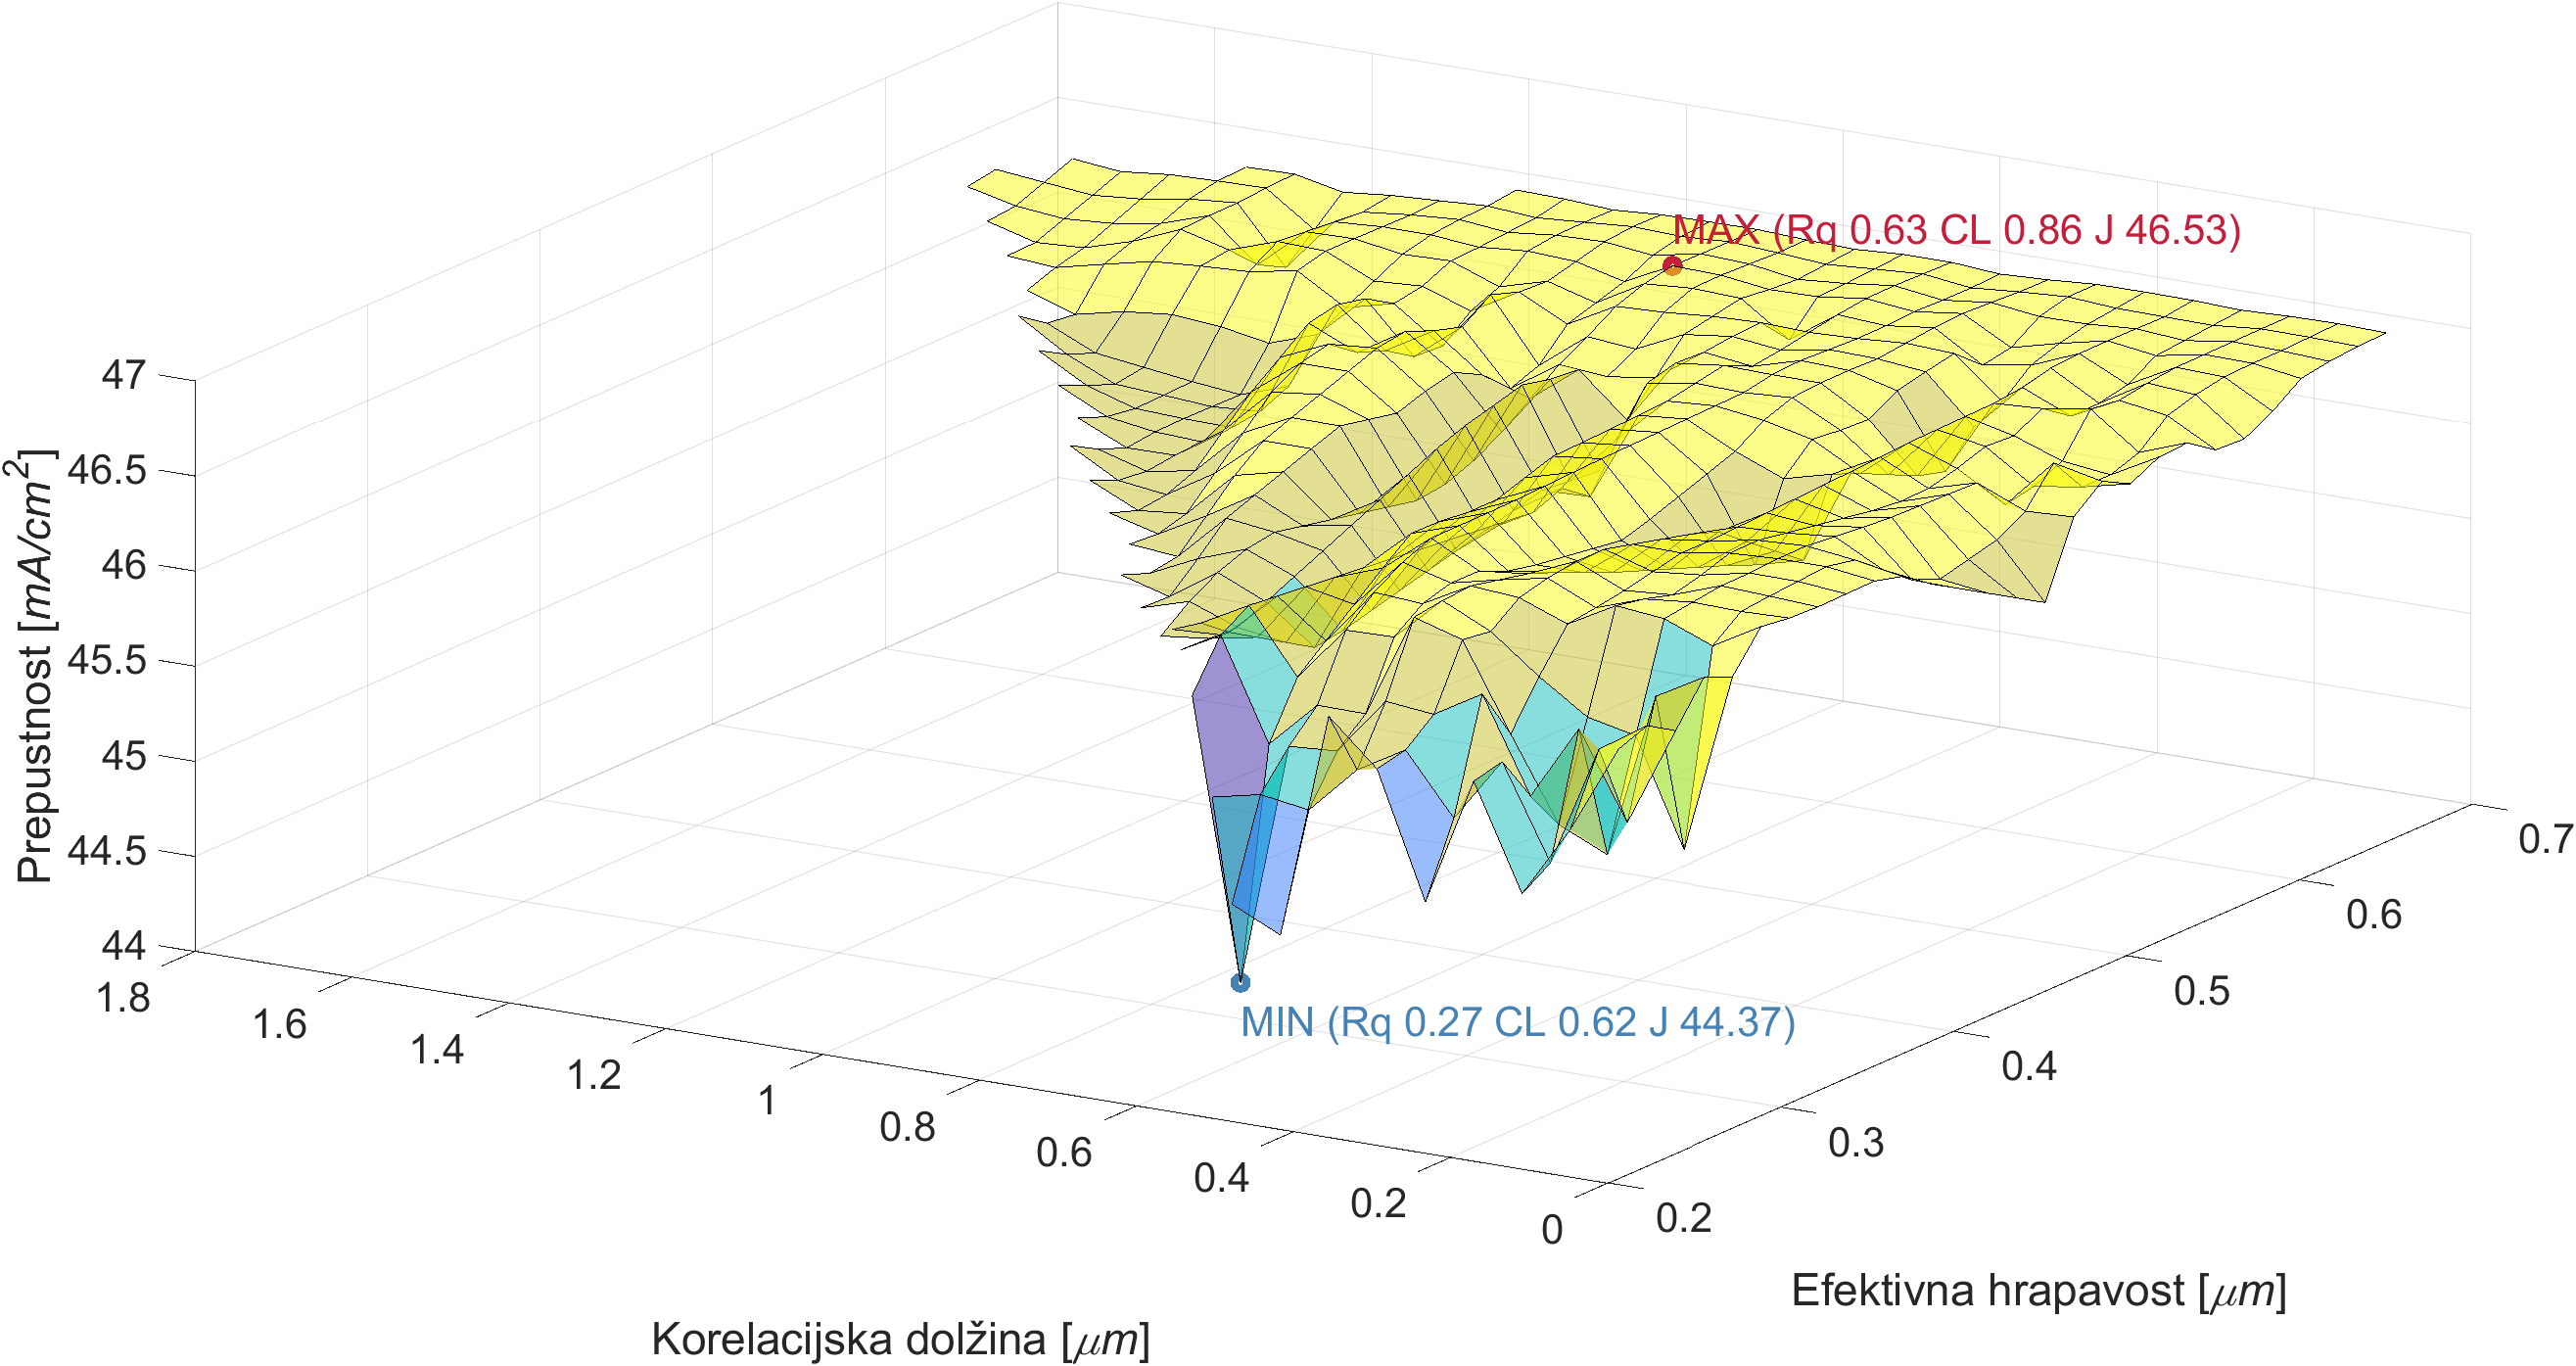
\includegraphics[width=150mm]{Slike/pre_air_Si.png}
    \caption{Prepustnost spoja zrak-silicij (spreminjanje površine)}
    \label{fig:pre_air_si_v}
\end{figure}

\begin{figure}[H]
    \centering
    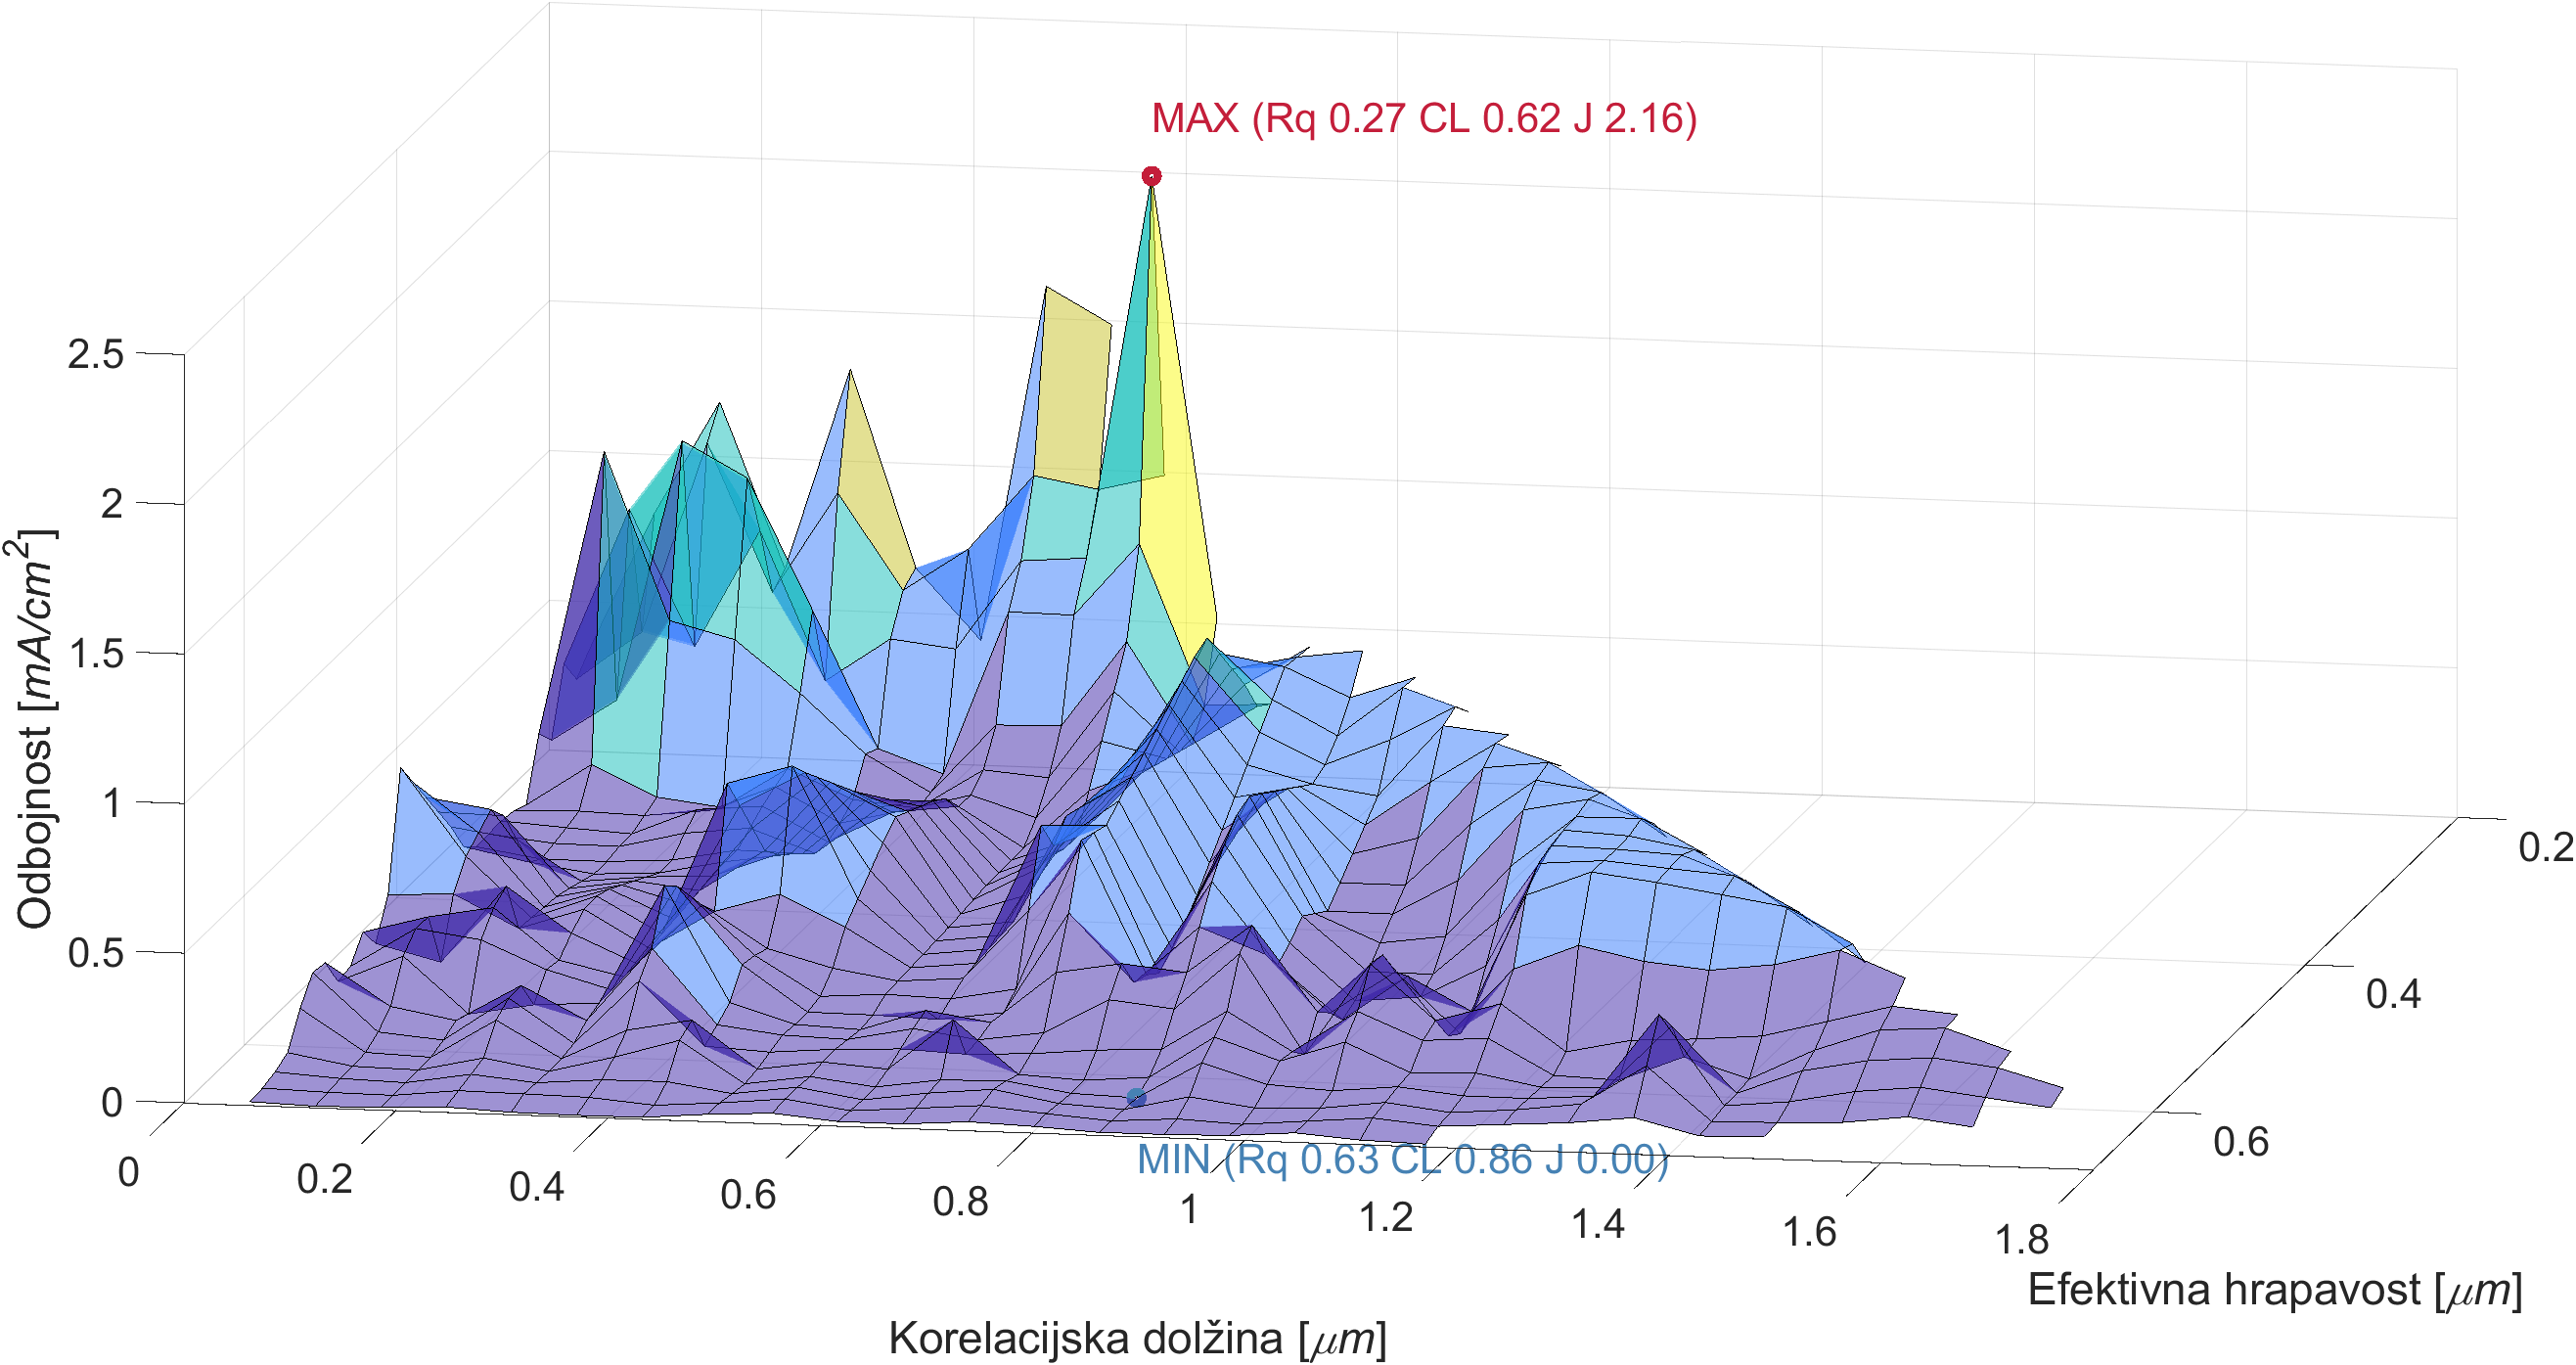
\includegraphics[width=150mm]{Slike/odb_air_Si.png}
    \caption{Odbojnost spoja zrak-silicij (spreminjanje površine)}
    \label{fig:odb_air_si_v}
\end{figure}

\subsubsection{Spoj silicij-zrak}

Komentarji grafov:

\begin{itemize}
    \item \underline{\hyperref[fig:pre_si_air_v]{Graf prepustnosti:}} Na sledečem grafu lahko opazimo maksimalno točko, ki je v tem primeru bolj naključno postavljena. Izrazita sta dva lokalna maksimuma, vsak na eni strani.

    \item \underline{\hyperref[fig:odb_si_air_v]{Graf odbojnosti:}} Na grafu odbojnosti veliko lepše vidimo značilnosti različnih površin. Opazimo, da je največja vrednost kratkostičnega toka v okolici najmanjših vrednosti le-tega. Omenjeno nam pove, da je na spoju silicij-zrak težje razpoznati logične vzorce razporeditve.
\end{itemize}


\begin{figure}[H]
    \centering
    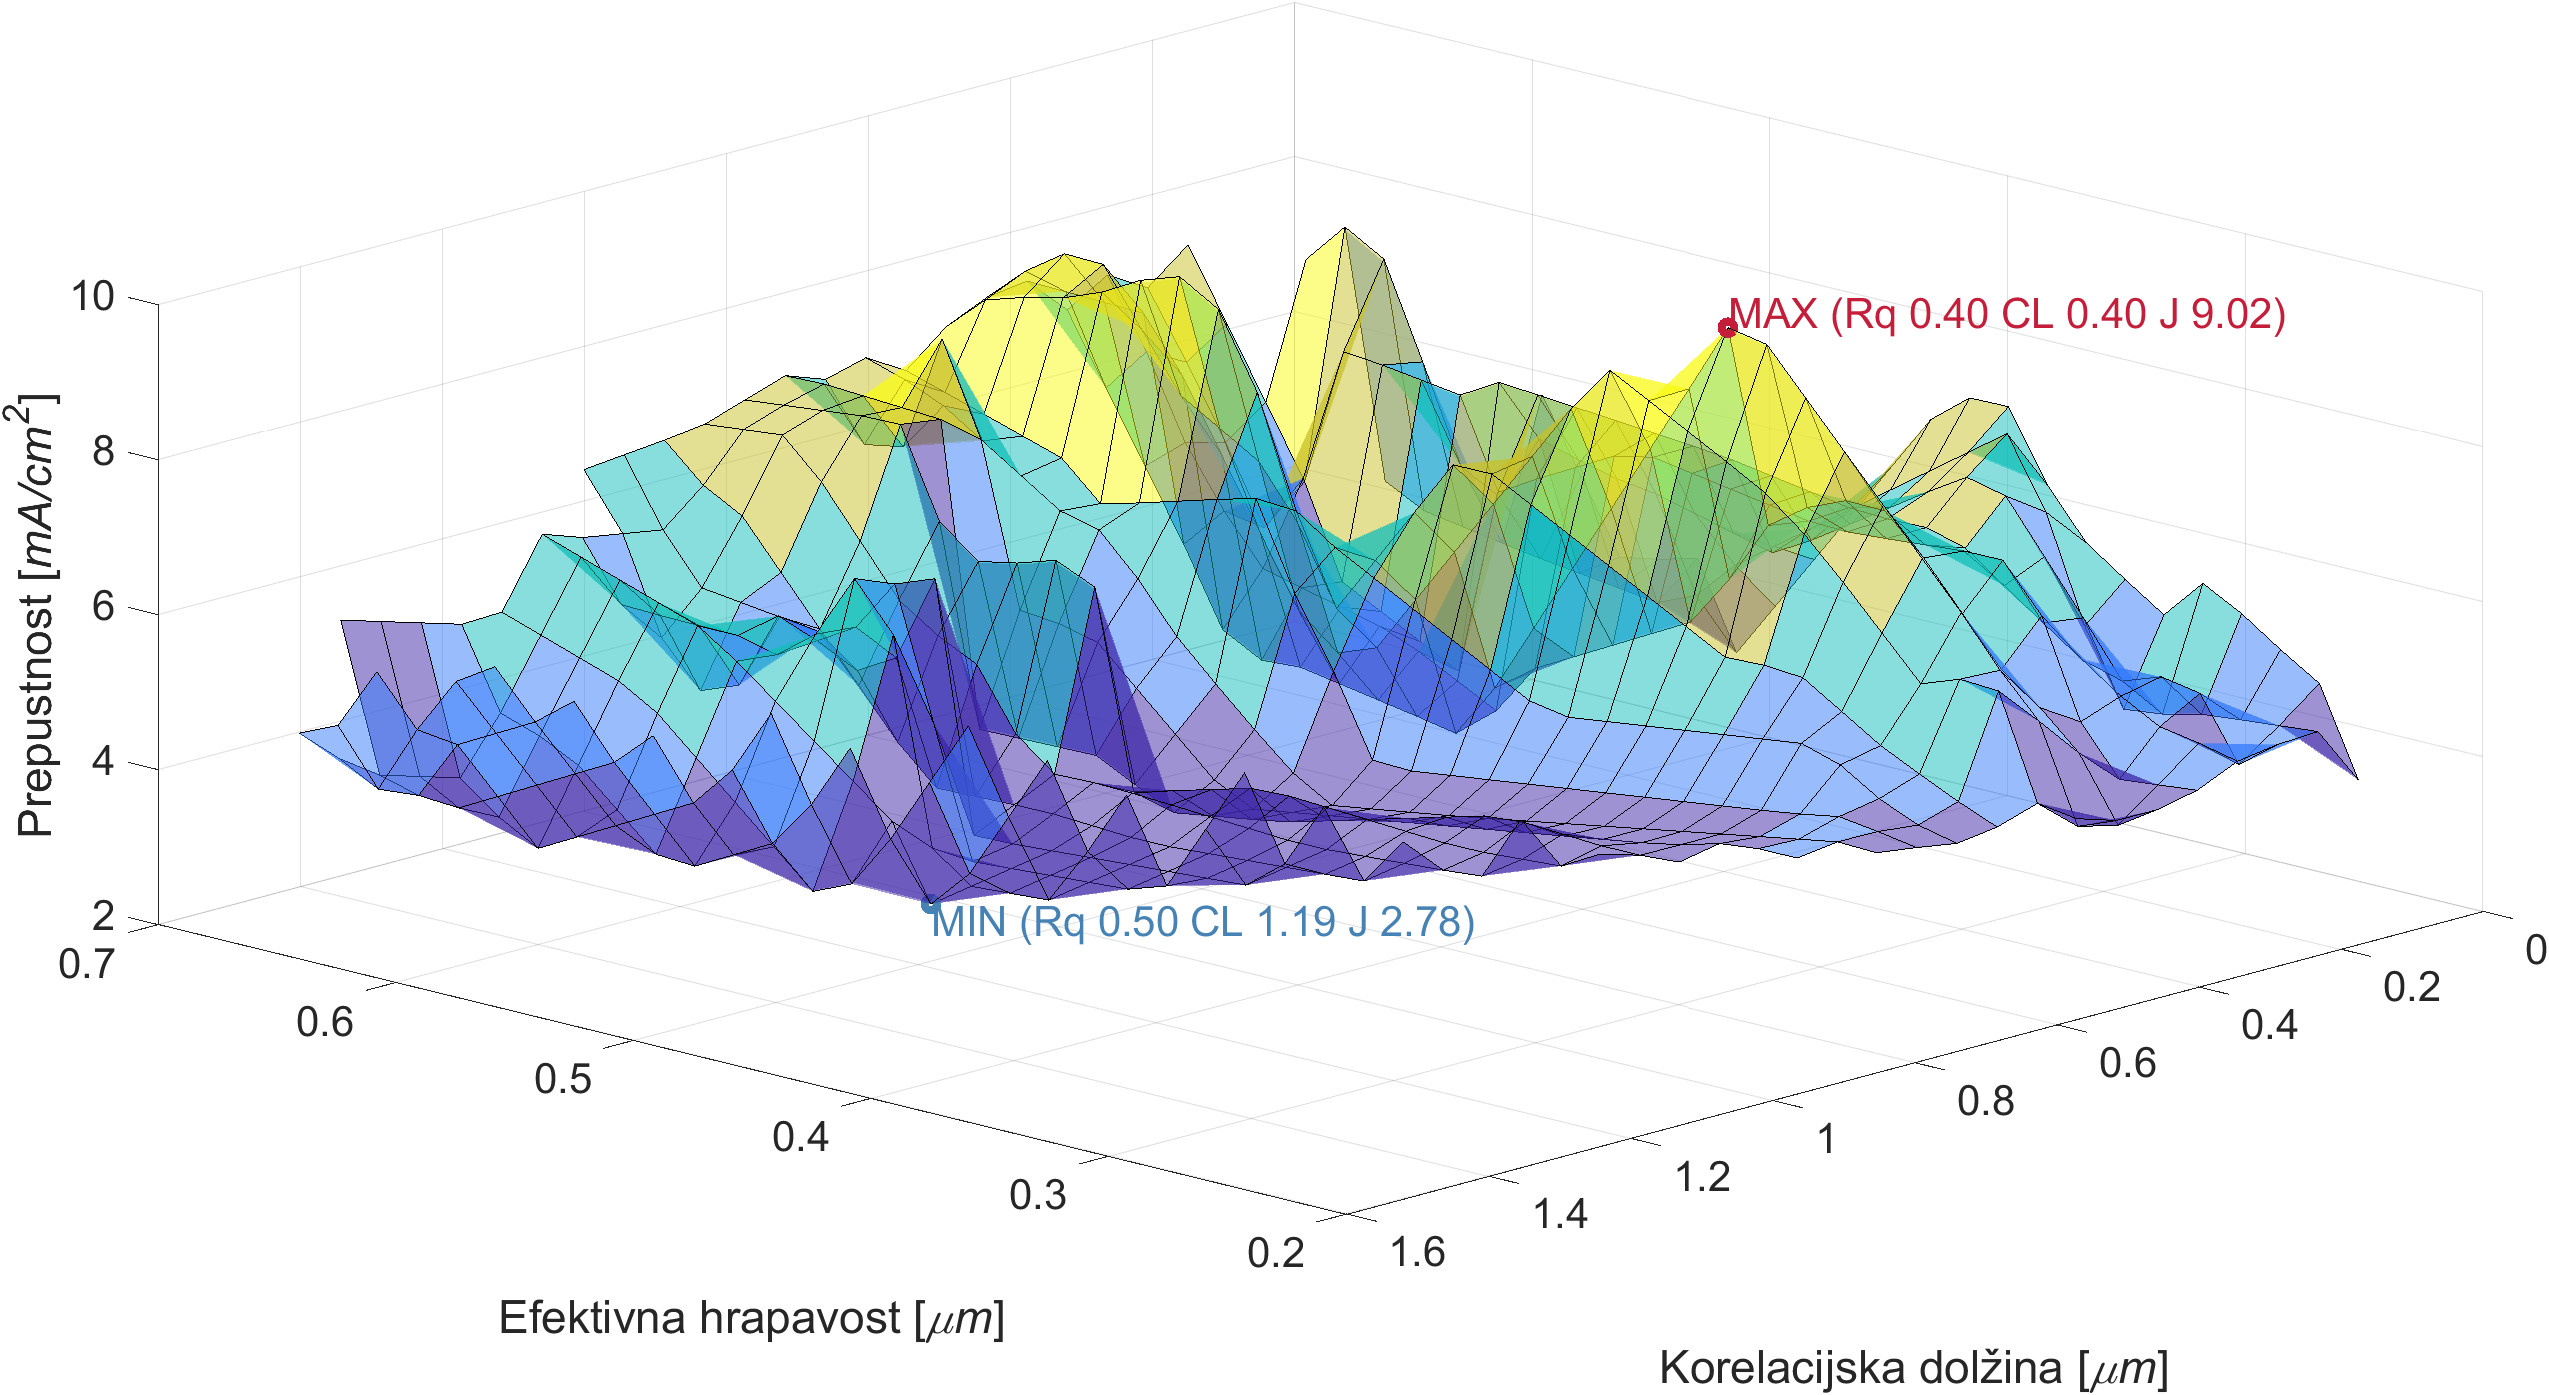
\includegraphics[width=150mm]{Slike/pre_Si_air.png}
    \caption{Prepustnost spoja silicij-zrak (spreminjanje površine)}
    \label{fig:pre_si_air_v}
\end{figure}

\begin{figure}[H]
    \centering
    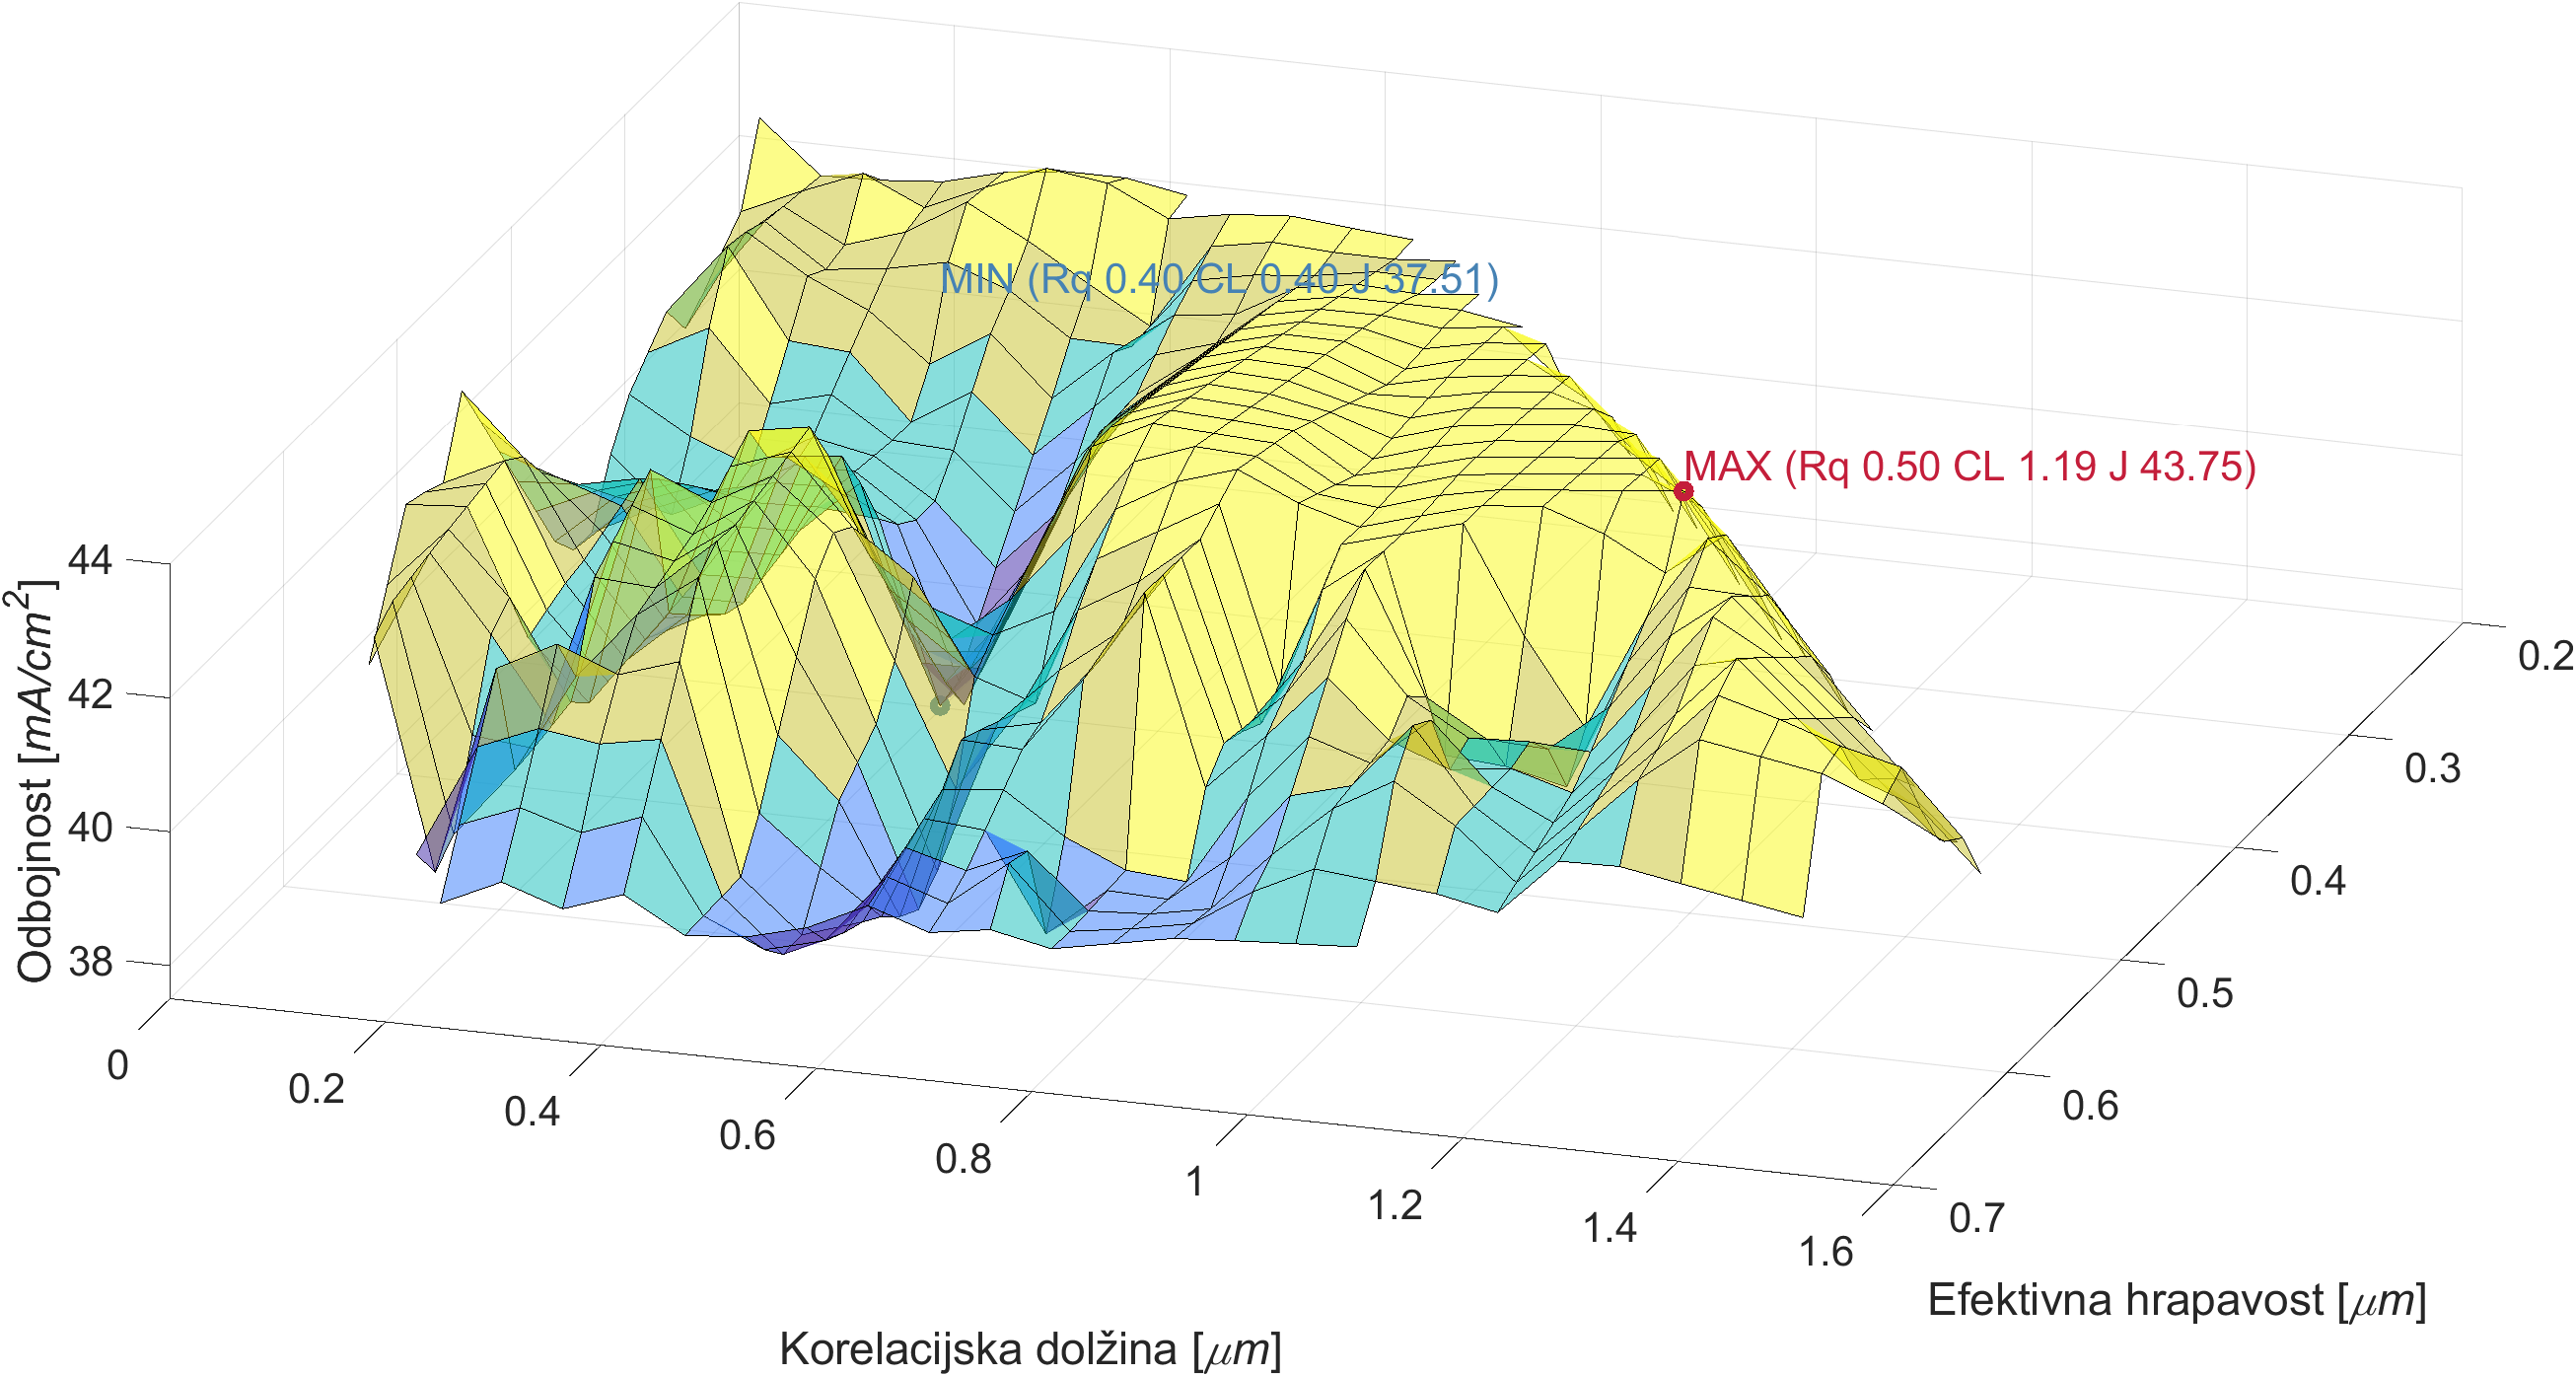
\includegraphics[width=150mm]{Slike/odb_Si_air.png}
    \caption{Odbojnost spoja silicij-zrak (spreminjanje površine)}
    \label{fig:odb_si_air_v}
\end{figure}


\section{Simulacije sončnih celic}

Simulacije smo izvedli na PERC sončnih celicah, saj zadostujejo kriterijem enostavnosti izdelave ter relativno malo plasti v strukturi ob povečanju izkoristka s pomočjo naključno hrapavih površin (glej poglavje \ref{percCelice}).

Zaradi časovne zahtevnosti izvedbe simulacij polnih struktur je bilo le-teh izvedenih nekoliko manj. Zaradi že prvotno nizkih amplitud naključno hrapavih površin se sledeče v PERC sončnih celicah izrazi kot relativno majhna razlika v vrednostih kratkostičnih tokov.

Komentar grafov:
\begin{itemize}
    \item \underline{\hyperref[fig:pre_PERC]{Graf prepustnosti:}} Na grafu lahko opazimo, da se nam z manjšanjem efektivne hrapavosti zniža prepustnost površine. Ob manjši korelacijski dolžini spet pride do delnega povečanja prepustnosti, a le-ta kmalu izzveni zaradi približevanja ničelnim vrednostim.
    
    \item \underline{\hyperref[fig:odb_PERC]{Graf odbojnosti:}} Pri grafu odbojnosti lahko opazimo ravno nasprotno. Ob povečevanju efektivne hrapavosti, se odbojnost manjša. Viden je lokalni greben pri korelacijski dolžini v okolici vrednosti \textbf{0,8}. Zanimivo pa je, da s preveliko korelacijsko dolžino odbojnost pade.
    
    \item \underline{\hyperref[fig:cSi]{Graf izkoristka plasti silicija:}} Omenjena plast je v PERC sončnih celicah optično aktivna, ker je zadolžena za pretvorbo svetlobne v električno energijo. Vrednosti kratkostičnih tokov tečejo med \textbf{38,6} ter \textbf{39,6} $\bf mA/cm^2$. Razlike so majhne, a hitro lahko opazimo, da je graf izredno podoben grafu odbojnosti, torej lahko sklepamo, da na izkoristek sončne celice pretežno vpliva odbojnost naključno hrapave površine.
\end{itemize}

\begin{figure}[H]
    \centering
    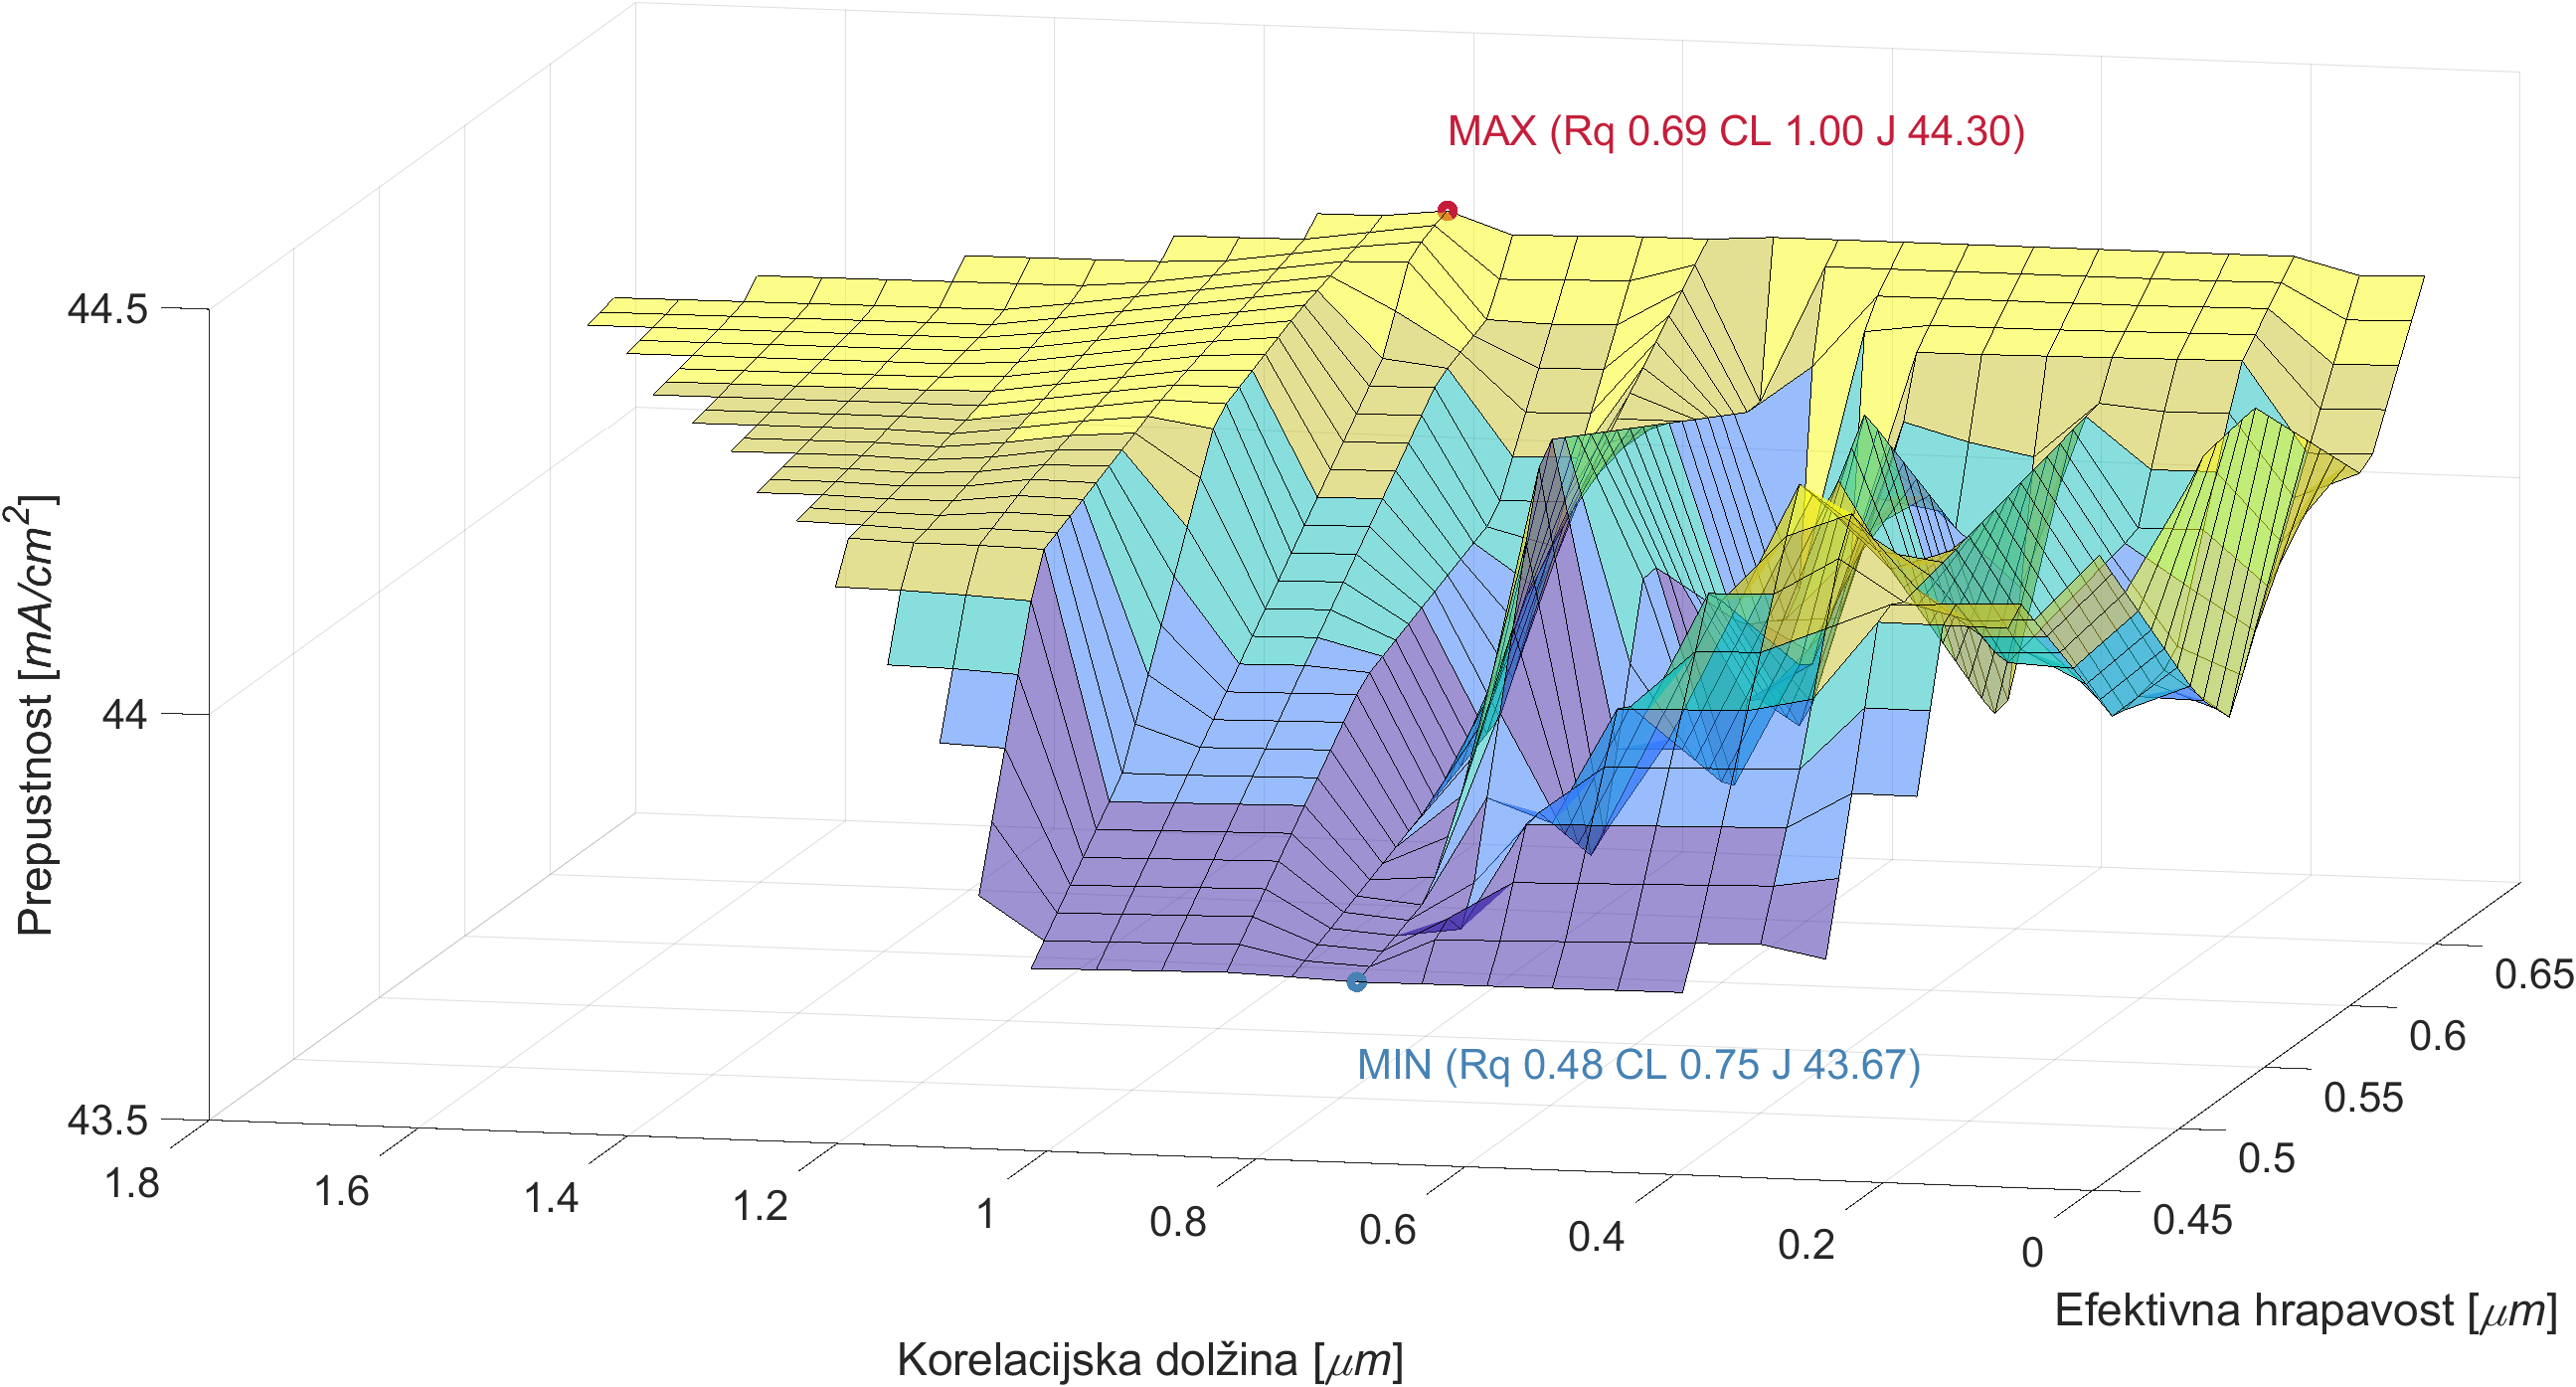
\includegraphics[width=150mm]{Slike/pre_PERC.png}
    \caption{Prepustnost PERC sončne celice}
    \label{fig:pre_PERC}
\end{figure}

\begin{figure}[H]
    \centering
    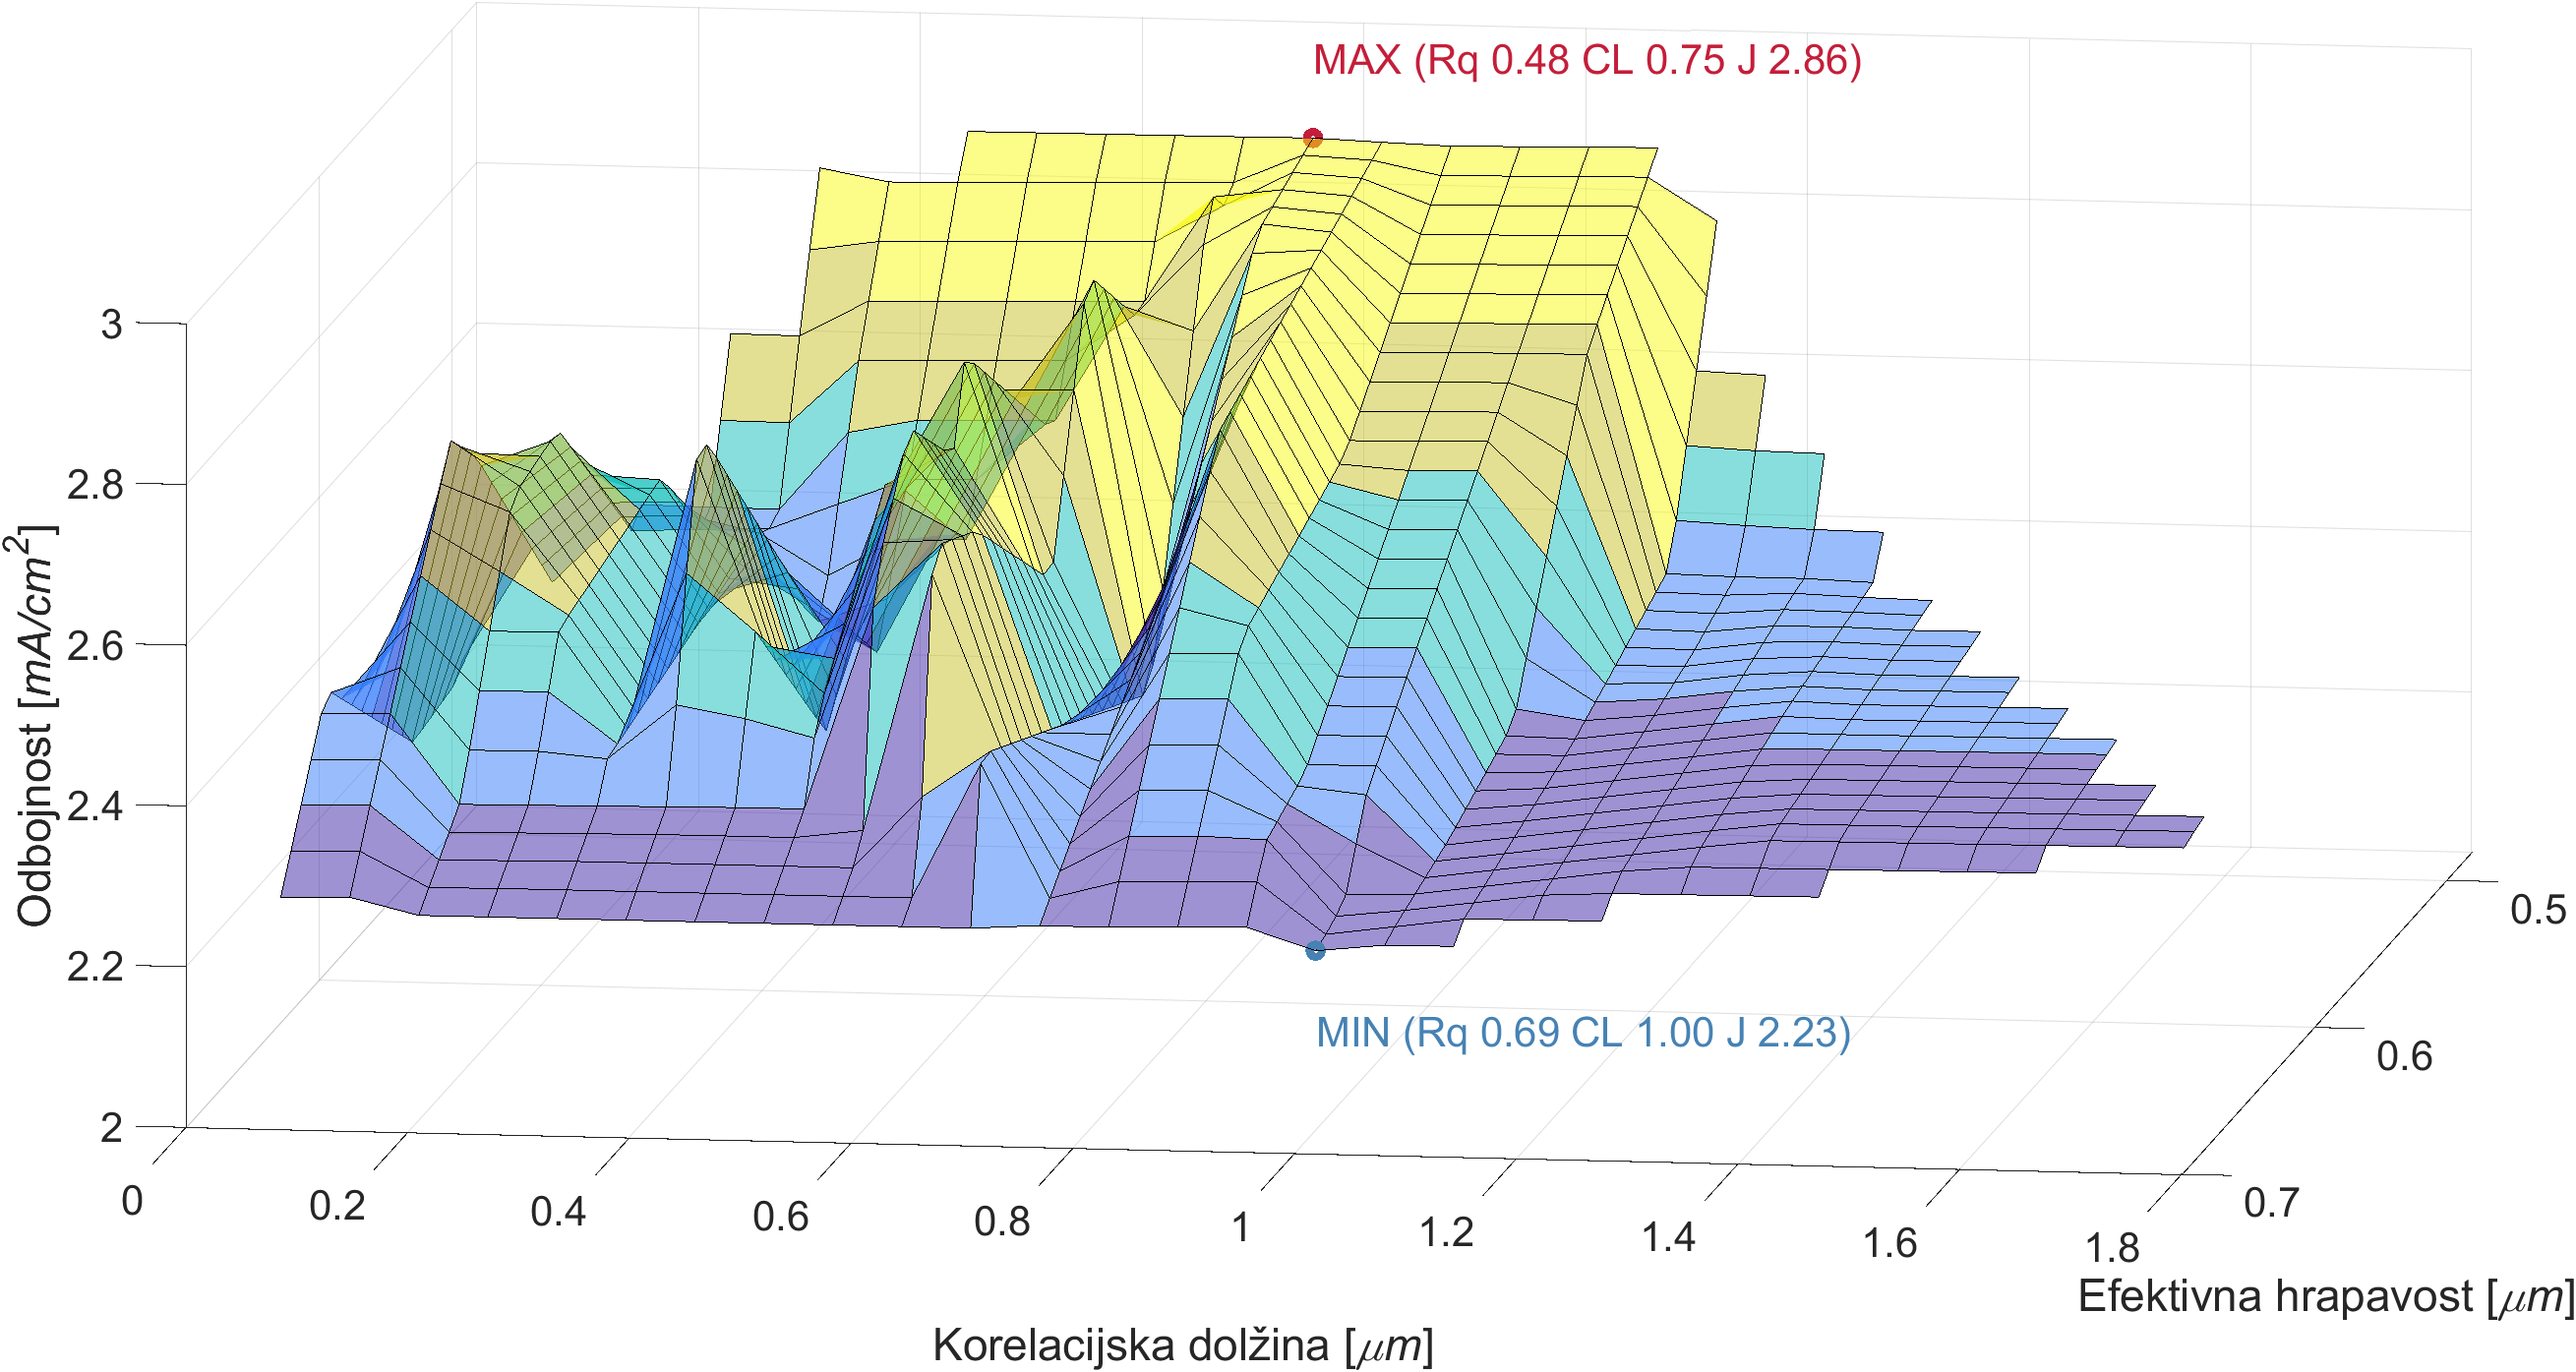
\includegraphics[width=150mm]{Slike/odb_PERC.png}
    \caption{Odbojnost PERC sončne celice}
    \label{fig:odb_PERC}
\end{figure}

\begin{figure}[H]
    \centering
    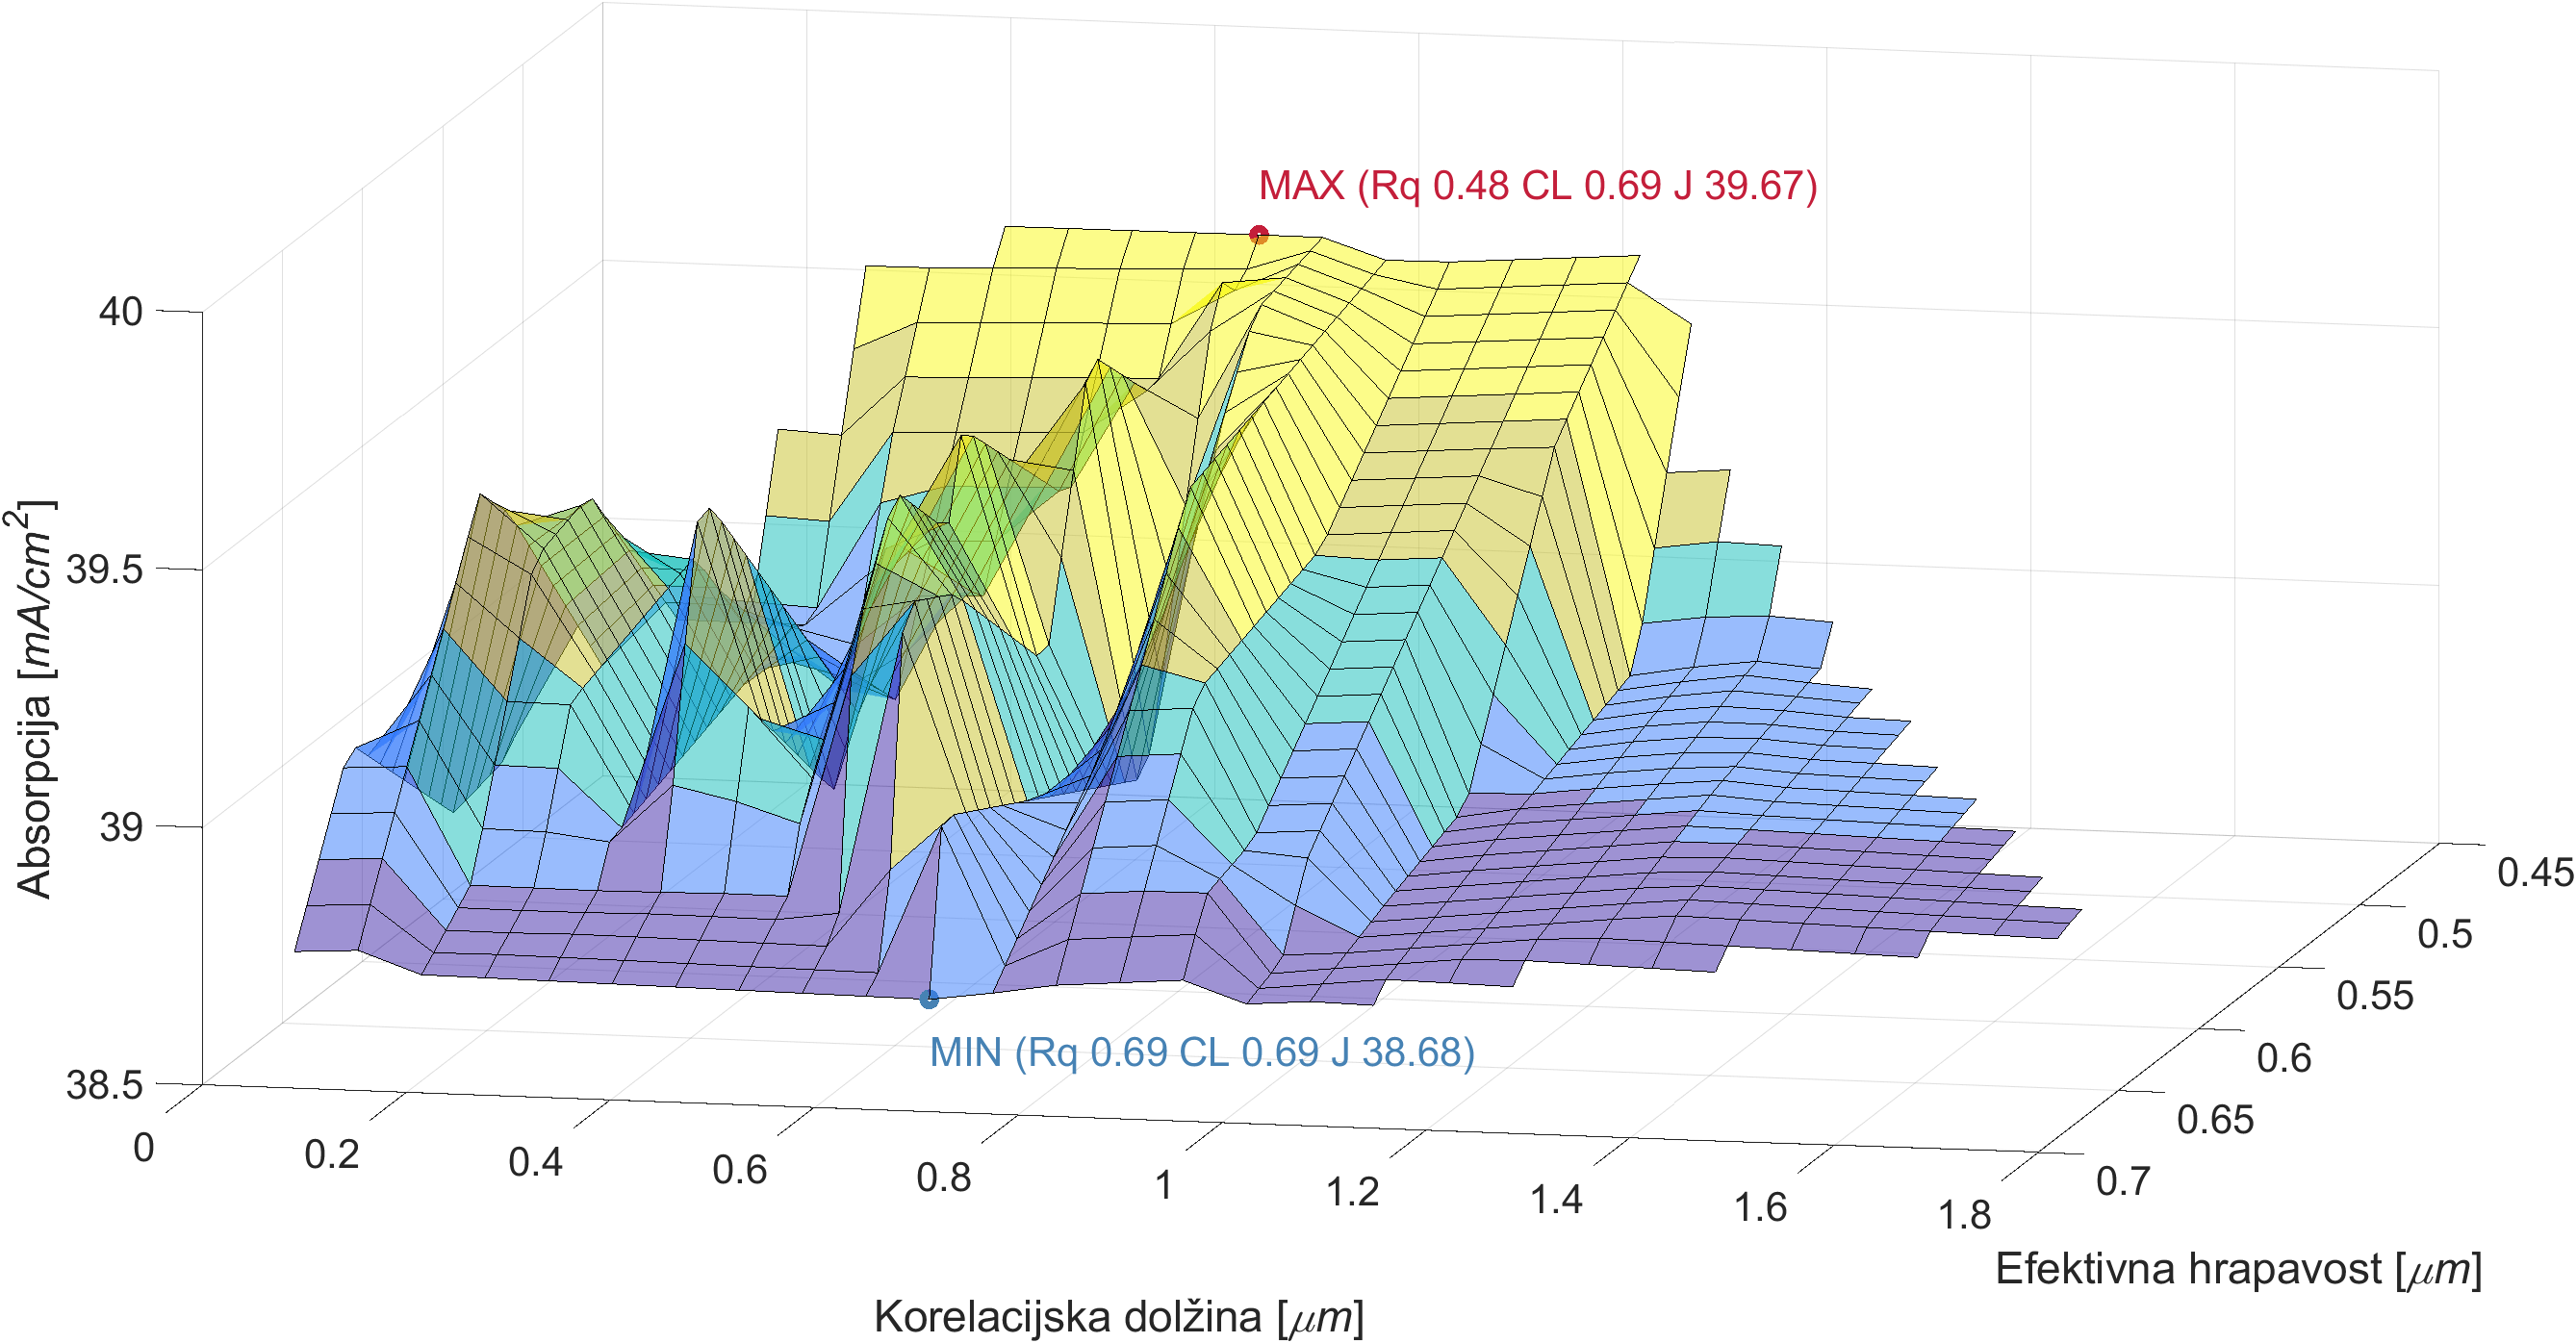
\includegraphics[width=150mm]{Slike/cSi_PERC.png}
    \caption{Izkoristek kratkostičnega toka v optično aktivni plasti silicija}
    \label{fig:cSi}
\end{figure}


\chapter{Zaključek}

Celotna tematika hrapavih površin ter njihov vpliv na različna področja je zelo obširna. V tej diplomski nalogi smo pokrili le manjši del vseh možnih variacij, tako struktur sončnih celic kot hrapavih površin.

\section{Končne ugotovitve}

 Dokazali smo, da lahko s pomočjo hrapavih površin spreminjamo izkoristke sončnih celic. Grafi standardnih deviacij so nam opredelili delovanje ter meje samega simulatorja CROWM. S spreminjanjem hrapavih površin smo preverili naključnost povezave med količinami efektivne hrapavosti, korelacijske dolžine ter primernih kratkostičnih tokov. Kljub neurejenosti podatkov je bilo mogoče opaziti splošne trende spreminjanja količin. Pri simulacijah PERC sončnih celic pa smo opazili, da se delež svetlobe kljub dobri optimizaciji vedno odbije.

\section{Težave}

Ena izmed glavnih težav, na katero smo naleteli šele ob koncu večine simulacij je čas trajanja simulacije. Omenjeni parameter se je pri kompleksnejši strukturi sončne celice podaljšal iz okvirno 1 do 2 uri na simulacijo na približno 24 ur. Prav tako se je čas simulacij podaljšal zaradi ločenega zaganjanja MATLAB skript iz PowerShell ukazne vrstice, a se le-to podaljšanje pri izvedbi ni preveč poznalo.

Zgornji problem bi lahko delno rešili z večimi simulacijami dvoplastnih struktur ter vnaprej določili kriterije, ki so nam na določenem spoju materialov pomembni.


\section{Nadaljnje delo}

Za optimalno izvajanje večjih količin simulacij bi bilo smiselno prestaviti generator naključno hrapavih površin in simulator CROWM v programski jezik/okolje, ki je primerno za paralelno izvedbo izračunavanja na grafični kartici. S tem bi omogočili pohitritev samih simulacij. Avtomatizacijsko skripto pa bi v tem primeru bilo smiselno spisati v programskem jeziku C, ki omogoča večjo robustnost kot PowerShell skripte.

Izvedli bi lahko izboljšavo avtomatizacijskega algoritma, saj trenutno samo zaporedno izvaja operacije. Najprej bi določili količino celotnega kratkostičnega toka ter glede na le-tega algoritmu določili nekaj začetnih parametrov, ki so spremenljivi. Algoritem bi nato z nekim grobim korakom šel čez vse spremenljive parametre ter našel lokalni maksimum. Sledeče bi rekurzivno izvedli v okolici vsakega lokalnega maksimuma, dokler ne bi dobili primernih vrednosti kratkostičnih tokov. \cite{IOPOPSC}


\cleardoublepage\phantomsection\addcontentsline{toc}{chapter}{Literatura}
\bibliographystyle{ieeetrslo}
\bibliography{literatura}







\end{document}
%%%%%%%%%%%%%%%%%%%%%%%%%%%%%%%%%%%%%%%%%%%%%%%%%%%%%%%%%%%%%%%%%%%%%%%%%%%%%%%%%%%%%%%%%%%%%%%%%%%%%%%%%%%%%%%%%%%%%%%%
